\PassOptionsToPackage{table}{xcolor}
\documentclass{beamer}

% xcolor and define colors -------------------------
\usepackage[table]{xcolor}

% https://www.viget.com/articles/color-contrast/
\definecolor{purple}{HTML}{5601A4}
\definecolor{navy}{HTML}{0D3D56}
\definecolor{ruby}{HTML}{9a2515}
\definecolor{alice}{HTML}{107895}
\definecolor{daisy}{HTML}{EBC944}
\definecolor{coral}{HTML}{F26D21}
\definecolor{kelly}{HTML}{829356}
\definecolor{cranberry}{HTML}{E64173}
\definecolor{jet}{HTML}{131516}
\definecolor{asher}{HTML}{555F61}
\definecolor{slate}{HTML}{314F4F}

% Mixtape Sessions
\definecolor{picton-blue}{HTML}{00b7ff}
\definecolor{violet-red}{HTML}{ff3881}
\definecolor{sun}{HTML}{ffaf18}
\definecolor{electric-violet}{HTML}{871EFF}

% Main theme colors
\definecolor{accent}{HTML}{00b7ff}
\definecolor{accent2}{HTML}{871EFF}
\definecolor{gray100}{HTML}{f3f4f6}
\definecolor{gray800}{HTML}{1F292D}


% Beamer Options -------------------------------------

% Background
\setbeamercolor{background canvas}{bg = white}

% Change text margins
\setbeamersize{text margin left = 15pt, text margin right = 15pt}

% \alert
\setbeamercolor{alerted text}{fg = accent2}

% Frame title
\setbeamercolor{frametitle}{bg = white, fg = jet}
\setbeamercolor{framesubtitle}{bg = white, fg = accent}
\setbeamerfont{framesubtitle}{size = \small, shape = \itshape}

% Block
\setbeamercolor{block title}{fg = white, bg = accent2}
\setbeamercolor{block body}{fg = gray800, bg = gray100}

% Title page
\setbeamercolor{title}{fg = gray800}
\setbeamercolor{subtitle}{fg = accent}

%% Custom \maketitle and \titlepage
\setbeamertemplate{title page}
{
    %\begin{centering}
        \vspace{20mm}
        {\Large \usebeamerfont{title}\usebeamercolor[fg]{title}\inserttitle}\\
        {\large \itshape \usebeamerfont{subtitle}\usebeamercolor[fg]{subtitle}\insertsubtitle}\\ \vspace{10mm}
        {\insertauthor}\\
        {\color{asher}\small{\insertdate}}\\
    %\end{centering}
}

% Table of Contents
\setbeamercolor{section in toc}{fg = accent!70!jet}
\setbeamercolor{subsection in toc}{fg = jet}

% Button
\setbeamercolor{button}{bg = accent}

% Remove navigation symbols
\setbeamertemplate{navigation symbols}{}

% Table and Figure captions
\setbeamercolor{caption}{fg=jet!70!white}
\setbeamercolor{caption name}{fg=jet}
\setbeamerfont{caption name}{shape = \itshape}

% Bullet points

%% Fix left-margins
\settowidth{\leftmargini}{\usebeamertemplate{itemize item}}
\addtolength{\leftmargini}{\labelsep}

%% enumerate item color
\setbeamercolor{enumerate item}{fg = accent}
\setbeamerfont{enumerate item}{size = \small}
\setbeamertemplate{enumerate item}{\insertenumlabel.}

%% itemize
\setbeamercolor{itemize item}{fg = accent!70!white}
\setbeamerfont{itemize item}{size = \small}
\setbeamertemplate{itemize item}[circle]

%% right arrow for subitems
\setbeamercolor{itemize subitem}{fg = accent!60!white}
\setbeamerfont{itemize subitem}{size = \small}
\setbeamertemplate{itemize subitem}{$\rightarrow$}

\setbeamertemplate{itemize subsubitem}[square]
\setbeamercolor{itemize subsubitem}{fg = jet}
\setbeamerfont{itemize subsubitem}{size = \small}


% Special characters

\usepackage{collectbox}

\makeatletter
\newcommand{\mybox}{%
    \collectbox{%
        \setlength{\fboxsep}{1pt}%
        \fbox{\BOXCONTENT}%
    }%
}
\makeatother





% Links ----------------------------------------------

\usepackage{hyperref}
\hypersetup{
  colorlinks = true,
  linkcolor = accent2,
  filecolor = accent2,
  urlcolor = accent2,
  citecolor = accent2,
}


% Line spacing --------------------------------------
\usepackage{setspace}
\setstretch{1.1}


% \begin{columns} -----------------------------------
\usepackage{multicol}


% Fonts ---------------------------------------------
% Beamer Option to use custom fonts
\usefonttheme{professionalfonts}

% \usepackage[utopia, smallerops, varg]{newtxmath}
% \usepackage{utopia}
\usepackage[sfdefault,light]{roboto}

% Small adjustments to text kerning
\usepackage{microtype}



% Remove annoying over-full box warnings -----------
\vfuzz2pt
\hfuzz2pt


% Table of Contents with Sections
\setbeamerfont{myTOC}{series=\bfseries, size=\Large}
\AtBeginSection[]{
        \frame{
            \frametitle{Roadmap}
            \tableofcontents[current]
        }
    }


% Tables -------------------------------------------
% Tables too big
% \begin{adjustbox}{width = 1.2\textwidth, center}
\usepackage{adjustbox}
\usepackage{array}
\usepackage{threeparttable, booktabs, adjustbox}

% Fix \input with tables
% \input fails when \\ is at end of external .tex file
\makeatletter
\let\input\@@input
\makeatother

% Tables too narrow
% \begin{tabularx}{\linewidth}{cols}
% col-types: X - center, L - left, R -right
% Relative scale: >{\hsize=.8\hsize}X/L/R
\usepackage{tabularx}
\newcolumntype{L}{>{\raggedright\arraybackslash}X}
\newcolumntype{R}{>{\raggedleft\arraybackslash}X}
\newcolumntype{C}{>{\centering\arraybackslash}X}

% Figures

% \imageframe{img_name} -----------------------------
% from https://github.com/mattjetwell/cousteau
\newcommand{\imageframe}[1]{%
    \begin{frame}[plain]
        \begin{tikzpicture}[remember picture, overlay]
            \node[at = (current page.center), xshift = 0cm] (cover) {%
                \includegraphics[keepaspectratio, width=\paperwidth, height=\paperheight]{#1}
            };
        \end{tikzpicture}
    \end{frame}%
}

% subfigures
\usepackage{subfigure}


% Highlight slide -----------------------------------
% \begin{transitionframe} Text \end{transitionframe}
% from paulgp's beamer tips
\newenvironment{transitionframe}{
    \setbeamercolor{background canvas}{bg=accent!40!black}
    \begin{frame}\color{accent!10!white}\LARGE\centering
}{
    \end{frame}
}


% Table Highlighting --------------------------------
% Create top-left and bottom-right markets in tabular cells with a unique matching id and these commands will outline those cells
\usepackage[beamer,customcolors]{hf-tikz}
\usetikzlibrary{calc, fit, shadows, arrows, arrows.meta, shapes.misc, shapes,decorations, decorations.pathreplacing, positioning}
\usepackage[most,skins]{tcolorbox}
\tcbuselibrary{breakable}
\tcbset{
  highlight math/.style={
    notitle, enhanced,
    on line, boxsep=2pt, left=0pt, right=0pt, top=0pt, bottom=0pt,
    colback = bgRaspberry, colframe = white,
  }
}

% To set the hypothesis highlighting boxes red.
\newcommand\marktopleft[1]{%
    \tikz[overlay,remember picture]
        \node (marker-#1-a) at (0,1.5ex) {};%
}
\newcommand\markbottomright[1]{%
    \tikz[overlay,remember picture]
        \node (marker-#1-b) at (0,0) {};%
    \tikz[accent!80!jet, ultra thick, overlay, remember picture, inner sep=4pt]
        \node[draw, rectangle, fit=(marker-#1-a.center) (marker-#1-b.center)] {};%
}

\usepackage{breqn} % Breaks lines

\usepackage{amsmath}
\usepackage{mathtools}

\usepackage{pdfpages} % \includepdf

\usepackage{listings} % R code
\usepackage{verbatim} % verbatim

% Video stuff
\usepackage{media9}

% packages for bibs and cites
\usepackage{natbib}
\usepackage{har2nat}
\newcommand{\possessivecite}[1]{\citeauthor{#1}'s \citeyearpar{#1}}
\usepackage{breakcites}
\usepackage{alltt}

% Setup math operators
\DeclareMathOperator{\E}{E} \DeclareMathOperator{\tr}{tr} \DeclareMathOperator{\se}{se} \DeclareMathOperator{\I}{I} \DeclareMathOperator{\sign}{sign} \DeclareMathOperator{\supp}{supp} \DeclareMathOperator{\plim}{plim}
\DeclareMathOperator*{\dlim}{\mathnormal{d}\mkern2mu-lim}
\newcommand\independent{\protect\mathpalette{\protect\independenT}{\perp}}
   \def\independenT#1#2{\mathrel{\rlap{$#1#2$}\mkern2mu{#1#2}}}
\newcommand*\colvec[1]{\begin{pmatrix}#1\end{pmatrix}}

\newcommand{\myurlshort}[2]{\href{#1}{\textcolor{gray}{\textsf{#2}}}}


\begin{document}

\begin{frame}[plain]  % Removes header/footer and gives you full vertical control
\vfill
\begin{center}
  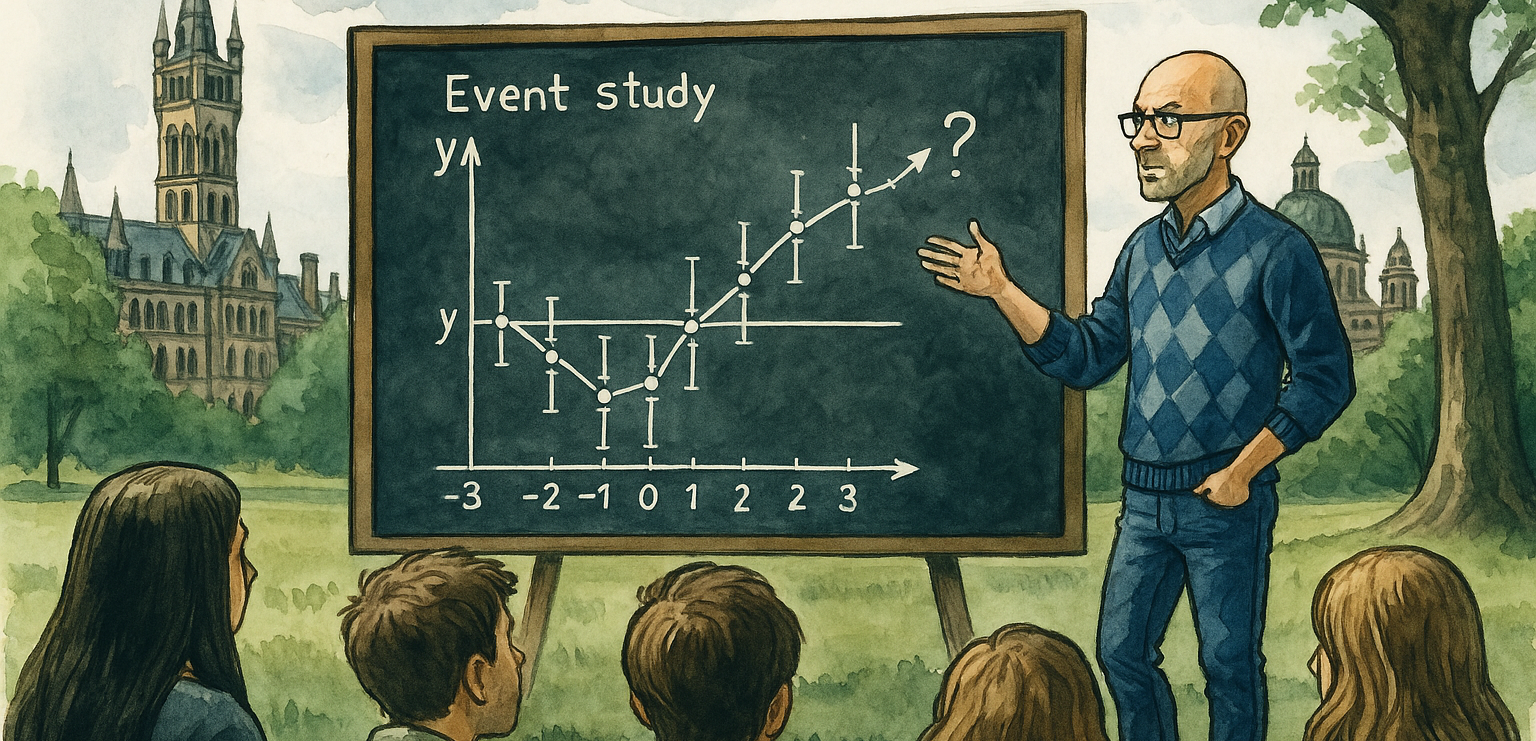
\includegraphics[width=0.85\linewidth]{./lecture_includes/banner_cropped}
\end{center}
\vfill
\end{frame}


% ---- Content ----


\section{Imputation DiD}

\subsection{Imputation based robust estimator}



\begin{frame}{Background}

\begin{itemize}

\item The origin of the robust diff-in-diff papers identifying pathologies in TWFE was Borusyak and Jaravel (2016) working paper
\item Both problems with static and dynamic specifications were discussed, and the identification of the ``already treated'' as controls
\item Paper remained in working paper until 2021 when Jan Speiss was brought on; the team developed a new estimator
\item We will focus primarily on the estimator, to avoid redundancies

\end{itemize}

\end{frame}

\begin{frame}{My Outline}

\begin{enumerate}
\item Discussion of their interpretation of ``basic'' DiD assumptions
\item Critique of TWFE OLS when strong assumptions don't hold
\item Introduction of new assumptions
\item Robust efficient imputation estimator
\end{enumerate}

\end{frame}


\begin{frame}{ATT parameter}

Unlike CS and SA, BJS has a unit-level treatment effect parameter as its target.  This is then aggregated to the ATT, but point is it starts lower.

\begin{eqnarray*}
\tau_w = \sum_{it \in \Omega_{1}}w_{it}\tau_{it} = w'_1\tau
\end{eqnarray*}

\bigskip

Note the weights -- they need not add up to one.  Weights could be $\frac{1}{N}$ for all $it \in \Omega_1$. We have a number of options. 


\end{frame}

\begin{frame}{Standard TWFE Assumptions}


\begin{itemize}
\item Like SA and dCDH, they both "reverse engineer" TWFE and they "forward engineer" a new estimator. 
\item First, the reverse engineering of TWFE which is unbiased under three main assumptions without covariates:
\begin{enumerate}
\item Parallel trends -- but it will have a fixed effects specification, not "four averages and three subtractions"
\item No anticipation
\item \textcolor{red}{Homogenous treatment effects}
\end{enumerate}
\item After we discuss this, we will discuss their new estimator
\end{itemize}

\end{frame}

\begin{frame}{TWFE Assumption 1: Parallel trends}

\textbf{Assumption 1: Parallel trends}. There exists fixed parameters $\alpha_i$ and $\beta_t$ in a $Y^0$ model:

$$Y_{it}^0 = \alpha_i + \beta_t + \varepsilon_{it}$$with $$E[\varepsilon_{it}]=0$$for all $it \in \Omega$. 

\end{frame}

\begin{frame}{TWFE Assumption 1: Parallel trends}

\begin{itemize}

\item Only imposes restrictions on $Y^0$, not treatment effects themselves. 
\item This is the same data generating process as in our \texttt{baker.do} simulation
\item It is not a parallel trends assumption expressed as "four averages and three subtractions" -- this is parallel trends in \emph{all pre-treatment periods}, not just from baseline to post
\item Notice that this is a twoway fixed effects model of $Y^0_{it}$ -- which will be important later
\end{itemize}

\end{frame}

\begin{frame}{TWFE Assumption 2: No anticipation}

\begin{itemize}
\item No anticipation rules out anticipatory behavior that would cause treatment effects to materialize even before the treatment occurred:$$Y_{it} = Y_{it}(0)$$ for all $it \in \Omega_0$. 
\item Notice how as an assumption, it literally imposes $\tau=0$ for all pre-treatment periods. 

\end{itemize}

\end{frame}



\begin{frame}{TWFE Assumption 3: Homogenous treatment effects}

\begin{itemize}
\item Up until now, these are the common diff-in-diff assumptions -- parallel trends and no anticipation -- but recall for unbiasedness, the canonical TWFE assumption also needs \textcolor{red}{homogenous treatment effects}
\item  Parallel trends and no anticipation are both restrictions on $Y^0$ -- parallel trends in the future, no anticipation in the past -- but homogenous treatment effects is $Y^1$ relative to $Y^0$:
\item  If we can assume something like homogenous treatment effects, parallel trends in all periods of your data, and NA, then you get unbiased estimate of a variance weighted ATT and smaller confidence intervals though new work suggests there are better methods (Chen, Sant'Anna and Chie 2025)
\end{itemize}

\end{frame}



\begin{frame}{Negative weighting and violations of Assumption 3}


\begin{itemize}
\item Goodman-Bacon (2021) like result -- if you estimate TWFE, have PT and NA, and have a single dummy ("static specification"), then the TWFE coefficient has \emph{negative weights}
\item And weights may not sum to 1 either
\item Hence the canonical TWFE estimator used in diff-in-diff with differential timing is not a "properly weighted average" of treatment effects, as some of the weights are negative (and maybe flip the sign)
\item Some find their illustration helpful, which I'll show now.
\end{itemize}

\end{frame}


\begin{frame}{Simple illustration}


\begin{table}[htb]\centering
\scriptsize
\caption{TWFE dynamics}
\centering
\begin{threeparttable}
\begin{tabular}{l*{2}{c}}
\toprule
\multicolumn{1}{l}{$E(y_{it})$ }&
\multicolumn{1}{c}{\textbf{$i=A$ }}&
\multicolumn{1}{c}{\textbf{$i=B$ }}\\
\midrule
t=1 & $\alpha_A$ & $\alpha_B$ \\
t=2 & $\alpha_A + \beta_2 + \delta_{A2}$ & $\alpha_B$ + $\beta_2$ \\
t=3 & $\alpha_A + \beta_3 + \delta_{A3}$ & $\alpha_B$ + $\beta_3$ + $\delta_{B3}$ \\
\midrule
Event date & $E_i=2$ & $E_i = 3$ \\
\bottomrule
\end{tabular}
\end{threeparttable}
\end{table}

Static: $\delta = \delta_{A2} + \frac{1}{2}\delta_{B3} - \frac{1}{2} \delta_{A3}$.  \\

\bigskip

Notice the negative weight on the furthest lag when dynamic and zero if constant. Similar to Bacon's negative weight on $\Delta ATT_U$.

\end{frame}


\begin{frame}{Short-run bias of TWFE}

\begin{itemize}
\item TWFE OLS has a severe short-run bias because the larger the effects in the long-run, the smaller the static TWFE coefficient will be
\item It's caused by ``forbidden comparisons'' (late to early treated) in differential timing setups
\item Forbidden comparisons create downward bias on long-run effects with treatment effect heterogeneity, \emph{but not with treatment effect homogeneity} 
\item It's a violation of assumption 3 -- heterogenous treatment effects
\end{itemize}

\end{frame}


\begin{frame}{Modifications of general model}


Modification of A1 to A1': $$ Y_{it}(0) = A'_{it} \lambda_i + X_{it}' \delta + \varepsilon_{it}$$

\bigskip

Assumption 4 is introduced (homoskedastic errors).  This is key, because they will be building an ``efficient estimator'' with BLUE like OLS properties. 

\bigskip

Using A1' to A4, we get the ``efficient estimator'' which is for all linear unbiased estimates of $\delta_W$, the unique efficient estimator $\widehat{\delta_W^*}$ can be obtained with 3 steps

\end{frame}


\begin{frame}{Role of the untreated observations}


\begin{quote}
``The idea is to estimate the model of $Y_{it}^0$ using the untreated observations and extrapolate it to impute $Y_{it}^0$ for treated observations'' (Borusyak, Jaravel and Speiss 2024)
\end{quote}

\bigskip 

\begin{quote}
``At some level, all methods for causal inference can be viewed as imputation methods, although some more explicitly than others.'' -- Imbens and Rubin (2015)
\end{quote}


\end{frame}

\begin{frame}{Steps}

Their solution is to estimate the $Y^0_{it}$ model using the control group only, similar to Heckman, Ichimura and Todd (1997) with covariates (though here it's with fixed effects)

\begin{enumerate}
\item Estimate expected $\widehat{Y^0}_{it}$ for all untreated observations using TWFE (i.e., $t_i<E_i$)
\item Impute $\widehat{Y^0}_{it}$ using those estimated fixed effects for the treatment group in the treated period
\item Subtract $\widehat{\delta}_{it} = Y_{it}^1 - \widehat{Y}_{it}^0$ to get individual treatment effects
\item Aggregate the estimated treatment effects into an ATT (e.g.,  $$\widehat{\delta}_W = \sum_{it}w_{it}\widehat{\delta}_{it}$$
\end{enumerate}

\end{frame}


\begin{frame}{Why is this working?}

\begin{itemize}
\item Think back to that original statement of the PT assumption -- you're modeling $Y(0)_{it}$. 
\item That is, without treatment -- so the potential outcomes do not depend on any treatment effect
\item Hence where we get treatment heterogeneity
\item We obtain consistent estimates of the fixed effects which are then used to extrapolate to the counterfactual units for all $Y(0)_{it \in \Omega_1}$
\item I think this is a very cool trick personally, and as it is still OLS, it's computationally fast and flexible to unit-trends, triple diff, covariates and so forth (though remember what we said about covariates)
\end{itemize}

\end{frame}


\begin{frame}{Comparisons to other estimators}

\begin{center}
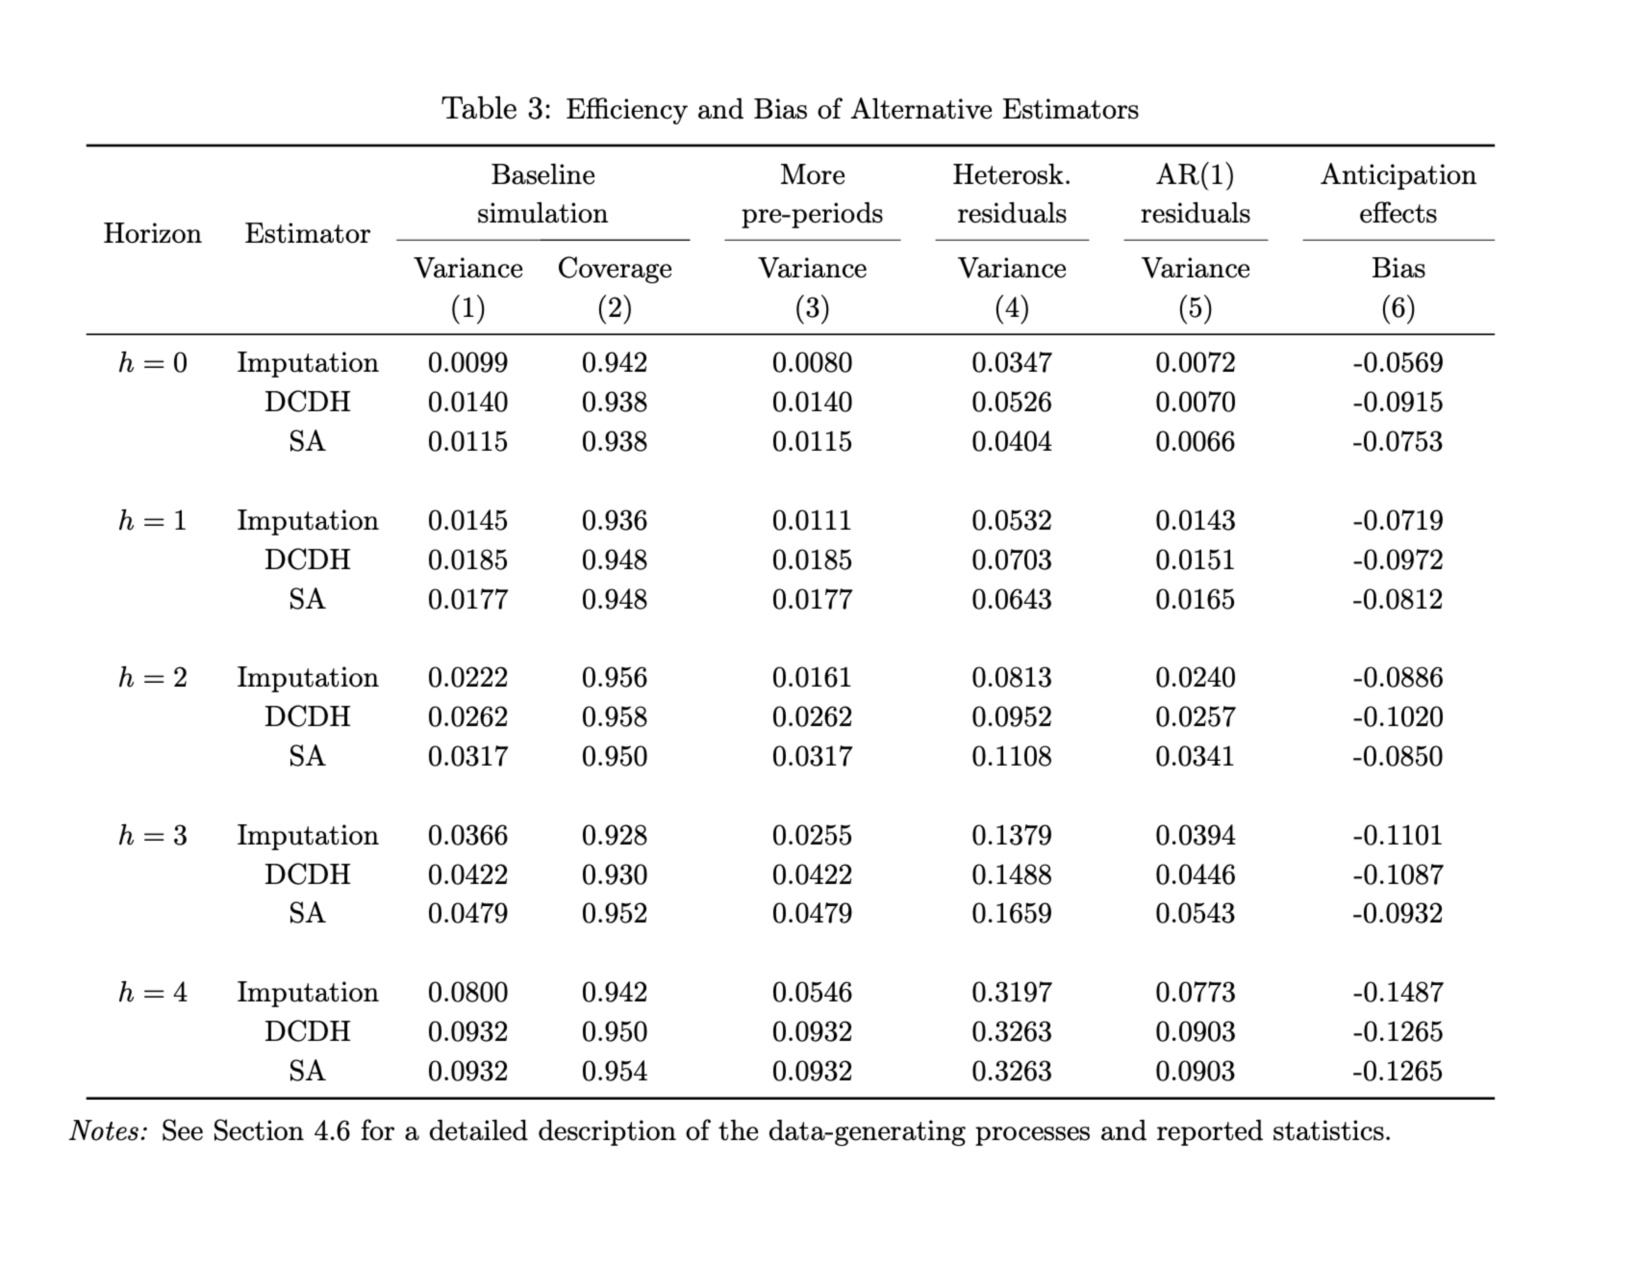
\includegraphics[scale=0.35]{./lecture_includes/bjs_sim.pdf}
\end{center}

\end{frame}

\begin{frame}{Returning to the minimum wage}

\begin{itemize}
\item Clemens and Strain (2021) implemented the BJS imputation estimator to estimate the effect of the minimum wage (post Great Recession) on employment
\item One comment abt the following graphics: BJS procedure does not have a ``base'' period in the same sense as the regression models do because it is not contrasting each period relative to some omitted group
\item Since it is imputing counterfactuals, we can calculate each period's effect
\end{itemize}

\end{frame}

\begin{frame}{BJS Results}

	\begin{figure}
	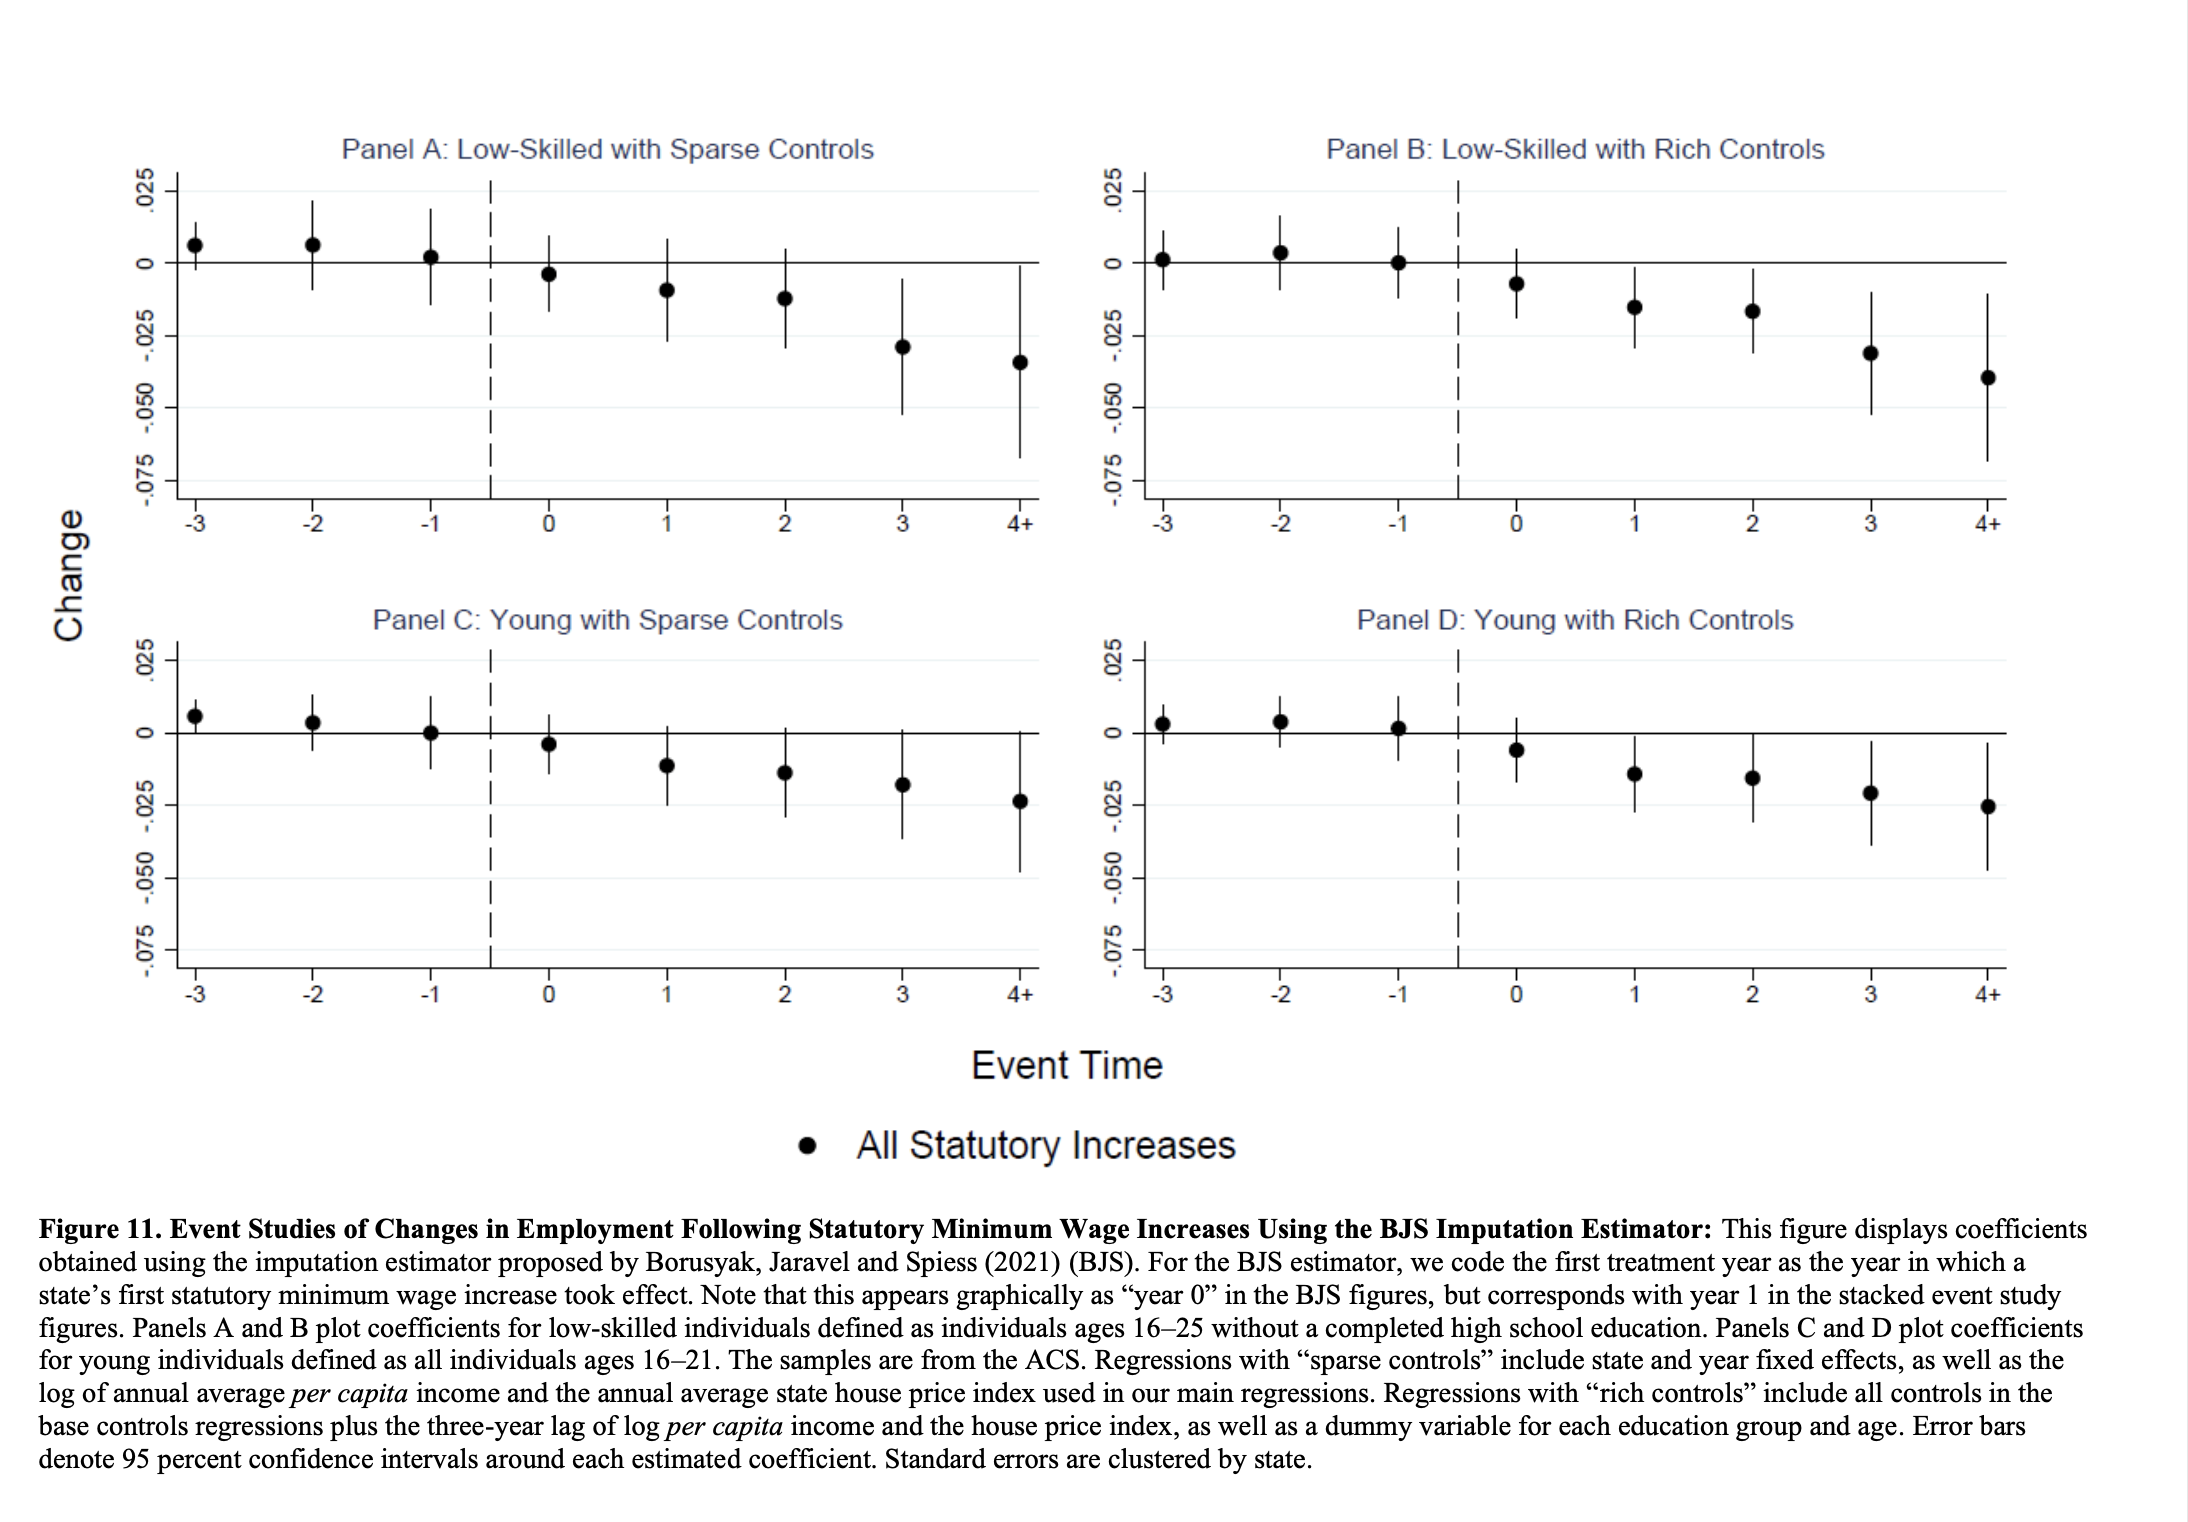
\includegraphics[scale=0.25]{./lecture_includes/Clemens_bjs_1.png}
	\end{figure}

\end{frame}

\begin{frame}{BJS Results}

	\begin{figure}
	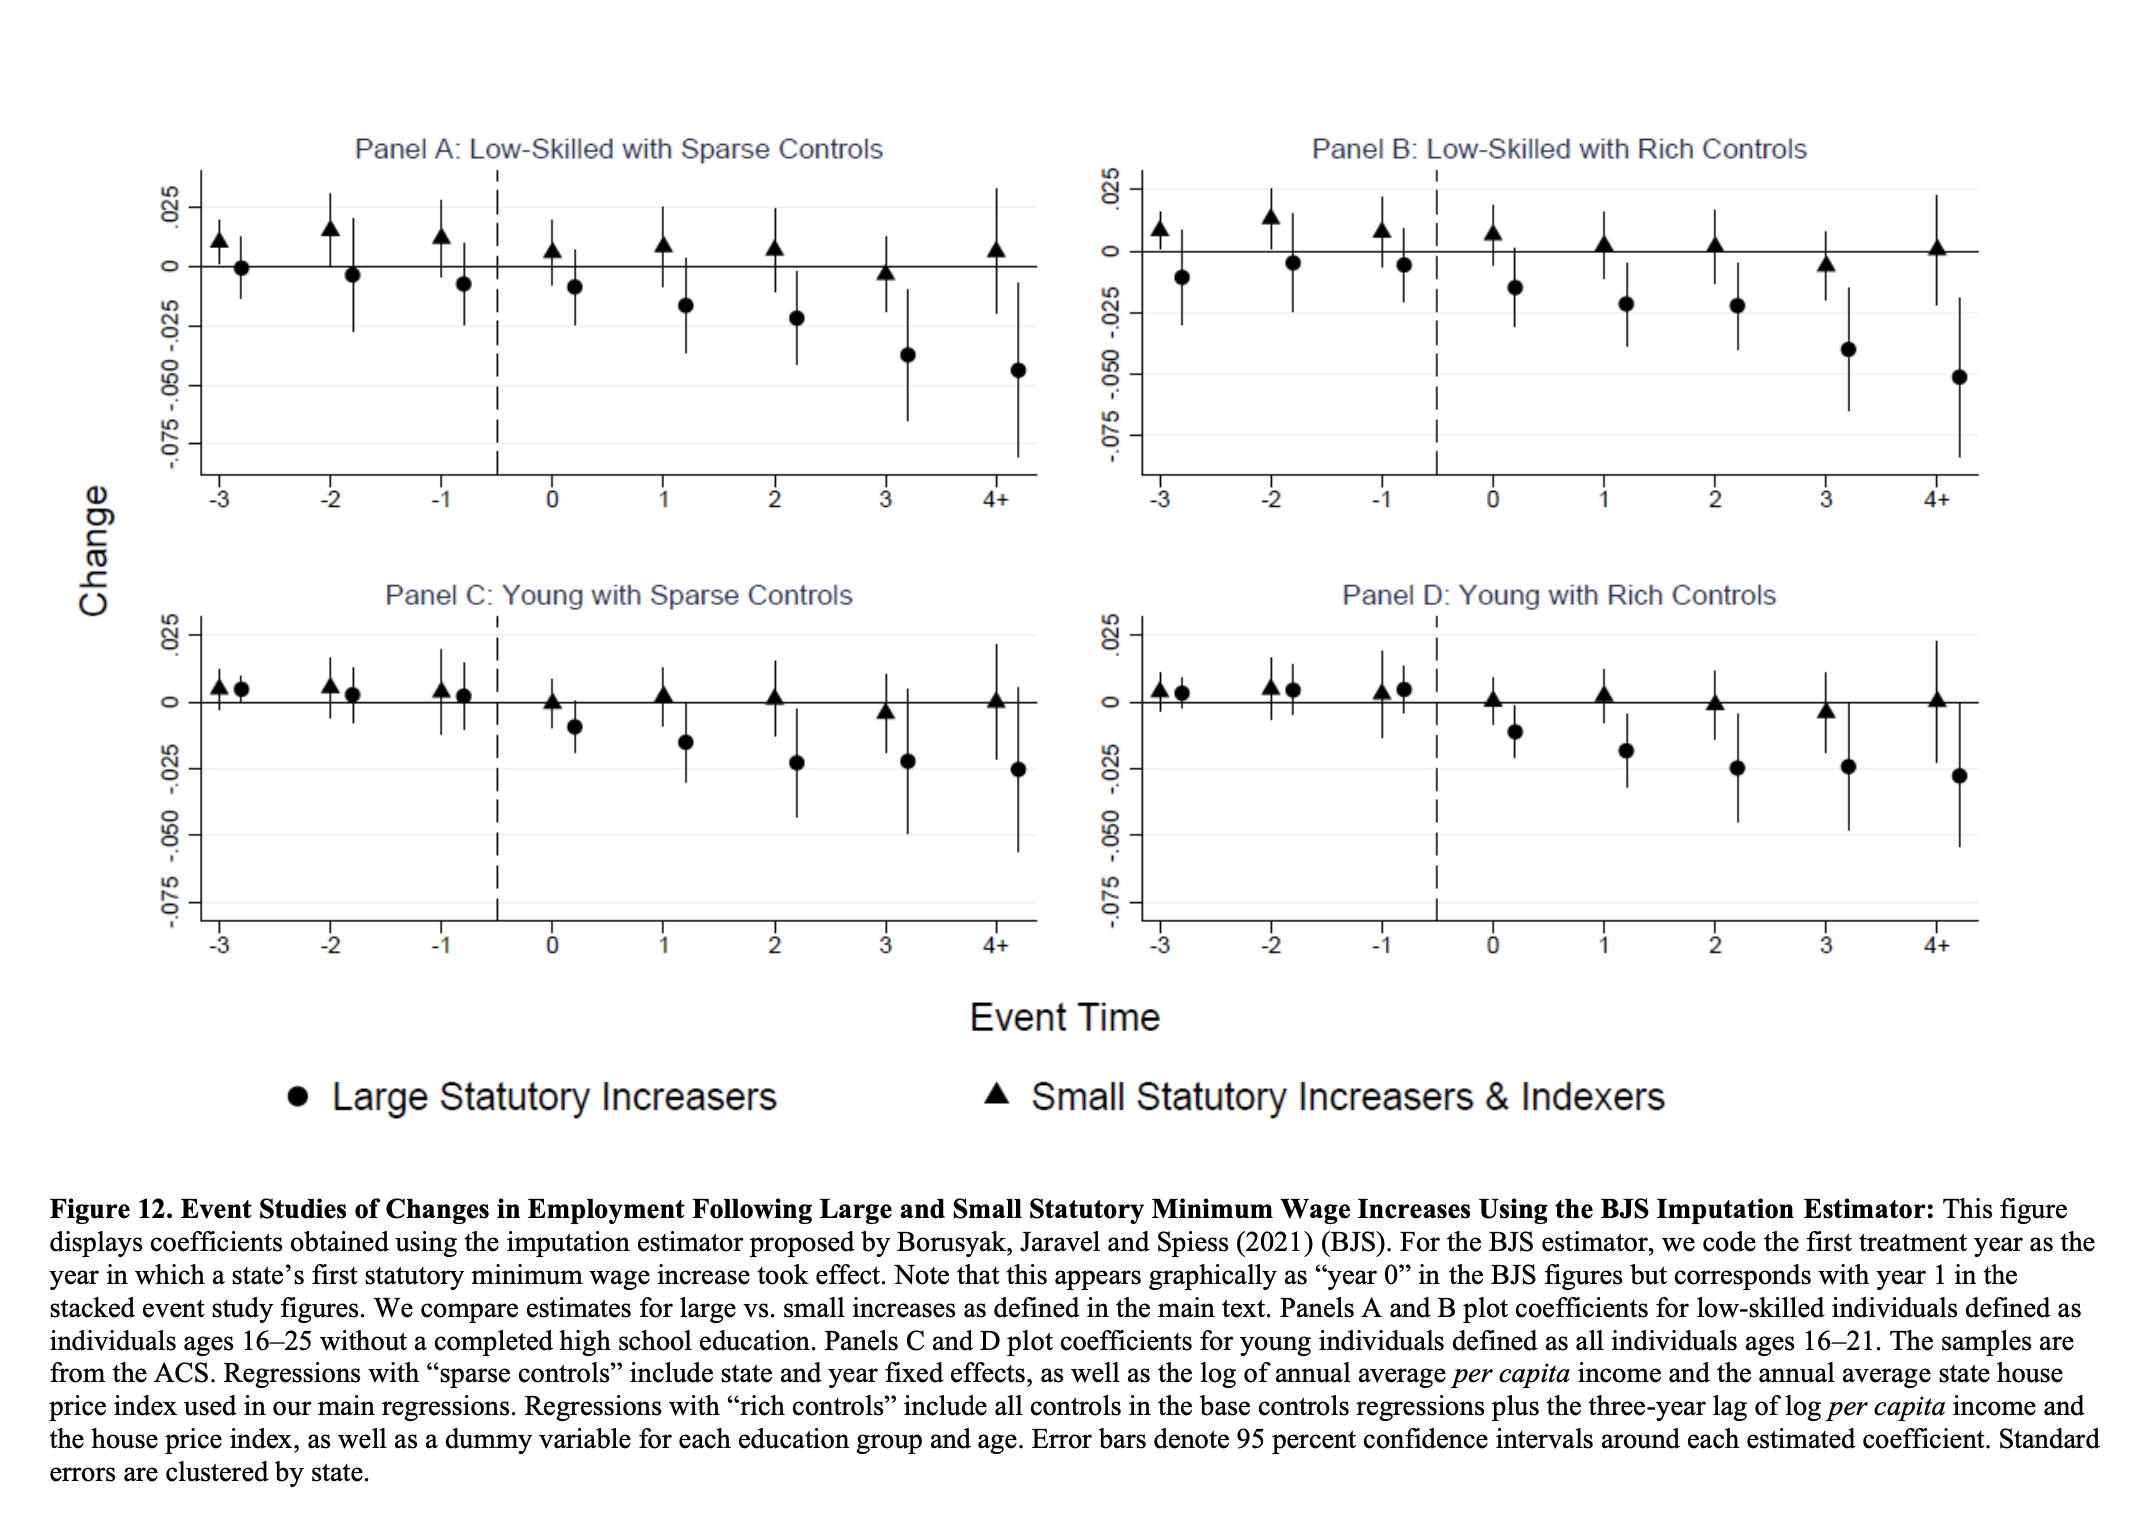
\includegraphics[scale=0.25]{./lecture_includes/Clemens_bjs_2.png}
	\end{figure}

\end{frame}

\begin{frame}{Comments abt the minimum wage study}

\begin{itemize}
\item Elasticity of employment with respect to minimum wage is -0.124 and -0.082 for those without high school and the young, respectively
\item Differences by size of minimum wage increase:
	\begin{itemize}
	\item Large increases (around \$2.90): own-wage elasticity is -1.01 for 16-25yo with less than HS and -0.41 for 16 to 21yo (large effects)
	\item Small increases (around \$1.90): own-wage elasticity is 0.46 (i.e., no employment effects)
	\item Inflation-index increases (around \$0.90): own-wage elasticity is 0.16 (no effect) and -0.17 (no effect)
	\end{itemize}
\end{itemize}

\end{frame}

\subsection{2SDiD}

\begin{frame}{Two Stage DiD}

\begin{quote}
``It seems natural that TWFE should identify the ATT'' -- Gardner (2021)
\end{quote}

\bigskip

It just seems like TWFE with a DiD will estimate the ATT with weights that we'll find intuitive.  Was this just a conjecture and was never true?  Why isn't this working?

\end{frame}



\begin{frame}{Two Stage DiD}

\begin{itemize}
\item Why does TWFE fail under differential timing? Violates strict exogeneity under heterogeneity
\item The logic of the failure suggests an obvious, but previously unknown, solution which is the 2SDiD
\item I'll explain 2SDiD, focus on the parallel trends implications, and show we can get a consistent and unbiased estimate of group and relative time fixed effects
\item If you can get consistent and unbiased estimates of group and relative time fixed effects, then you can delete them and run normal analysis
\end{itemize}

\end{frame}

\begin{frame}{Background}

\begin{itemize}
\item By now, we all agree that TWFE just doesn't handle heterogeneity under differential timing very well
\item We've seen in the Goodman-Bacon decomposition why -- it's caused by TWFE implicitly calculating late to early 2x2s, which are a source of bias
\item But some of you are coming straight from a panel econometrics course that maybe didn't use potential outcomes notation
\item Isn't strict exogeneity enough for consistent estimates?  What then does strict exogeneity have to do with heterogeneity and differential timing?
\end{itemize}

\end{frame}

\begin{frame}{High level discussion}

\begin{itemize}
\item TWFE identifies the ATT when the heterogeneous effects are distributed equally across all groups and periods, but since that is a knife-edge situation, it is likely that TWFE will not in our applications meet this special scenario
\item In the two group case, that is what happens though which is why TWFE worked fine there
\item Metaphorically, the two group case that we always used to pin our intuition of what DiD was doing was the exception not the rule
\item Goodman-Bacon (2021) shows the problem is caused by late-to-early comparisons; Gardner (2021) will show that the problem is misspecification
\item Think of these as different perspectives on the same problem
\end{itemize}

\end{frame}

\begin{frame}{Model misspecification}

\begin{quote}
``Misspecified DiD regression models project heterogenous treatment effects onto group and period fixed effects rather than the treatment status itself''
\end{quote}

\bigskip

Spoiler: This analysis of the problem suggests solution -- why don't we remove those?

\end{frame}


\begin{frame}{2SDiD}

\begin{itemize}
\item First stage -- estimate the group and relative time fixed effects using only the $D=0$ observations
\item Second stage -- using predicted values based off those fixed effect coefficients, run your model off the transformed outcome 
\item Get the standard errors right just like 2SLS by taking the first stage into account (uses GMM)
\end{itemize}

\end{frame}

\begin{frame}{More high level}

\begin{itemize}
\item The second step recovers the average difference in outcomes between treated and untreated units after removing group and period fixed effects
\item Strong parallel trends assumption compared to CS and SA, but unclear if this is a big deal in general
\end{itemize}

\end{frame}

\begin{frame}{Notation}

$i$: panel units \\
$t$: calendar time -- think of real dates\\
$g\in \{0,1, \dots , G \}$ -- groups\\
$p \in \{0,1, \dots , P \}$  -- relative time or ``periods''\\

\bigskip

Periods are successive.  Group 0 -- never treated. Group 1 -- treated in period 1, 2, and on.  Group 2 -- treated in period 2, etc.

\end{frame}

\begin{frame}{Parameters}

\begin{eqnarray*}
\beta_{gp} = E \bigg [ Y^1_{gpit} - Y^0_{gpit} | g,p \bigg ]
\end{eqnarray*}

\bigskip

It's a group-time ATT but expressed in a more traditional econometric notation that you could easily find in Wooldridge or some such

\end{frame}

\begin{frame}{Modeling basics}

Under parallel trends, mean outcomes will satisfy the following equation

\bigskip

\begin{eqnarray*}
E \bigg [ Y_{gpit} | g,p,D_{gp} \bigg ] = \lambda_g + \gamma_p + \beta_{gp} D_{gp}
\end{eqnarray*}

\bigskip

In two-group, group and period effects are eliminated with dummies because TWFE uses dummies to demean across multiple dimensions. Then TWFE identifies ATT.  But this does not hold when average effects vary across group and period. There are many ways to express a treatment effect's across group and time, but Gardner presented it as a weighted average of the coefficients for only that group-period situation:

\begin{eqnarray*}
E \bigg (\beta_{gp} | D_{gp}=1 \bigg ) = E \bigg (Y^1_{gpit} - Y^0_{gpit} | D_{gp}=1 \bigg )
\end{eqnarray*}

\end{frame}


\begin{frame}{Strict exogeneity violation}

Rewriting the above we get:

\begin{eqnarray*}
E \bigg [ Y_{gpit} | g,p, D_{gp} \bigg ] &=& \lambda_g + \gamma_p + E \bigg [\beta_{gp} | D_{gp} =1 \bigg ] D_{gp} \\
&& \bigg [\beta_{gp} - E ( \beta_{gp} | D_{gp} = 1 ) \bigg ] D_{gp}
\end{eqnarray*}

\bigskip

The problem is there's this weird new error term and it isn't mean zero under heterogenous treatment effects spread across group and period.  Unlike the two group case, the coefficient on $D_{gp}$ from TWFE doesn't identify the average $E(\beta_{gp} | D_{gp}=1)$ 

\bigskip

So let's see Gardner's solution, but note -- his solution was suggested by the problem itself. Gardner is thoughtful and observant.

\end{frame}

\begin{frame}{DiD regression estimand}

\begin{itemize}
\item So if TWFE isn't recovering $E(\beta_{gp} | D_{gp} = 1)$, then what is it recovering?
\item He shows that under PT, the coefficient on $D_{gp}$ is:

\begin{eqnarray*}
\beta^* = \sum_{g=1}^G \sum_{p=g}^P w_{gp}\beta_{gp}
\end{eqnarray*}

\item So then -- what are the weights $w_{gp}$?  They are variance weights 
\end{itemize}

\end{frame}

%\begin{frame}{Weights}

%\footnotesize
%\begin{eqnarray*}
%w_{gp} = \frac{ \bigg \{ [ 1-P(D_{gp}=1|g) ] - [P(D_{gp}=1|p) -  P(D_{gp}-1) ] \bigg \} P(g,p)}{
%\sum_{g=1}^G \sum_{p=g}^P \bigg \{ [ 1-P(D_{gp}=1 | g) ] - [P(D_{gp}=1 | p) - P(D_{gp}=1) ] \bigg \}P(g,p)}
%\end{eqnarray*}

%Terms: 
%\begin{itemize}
%\item $P(D_{gp}=1|p)$: share of units treated in period $p$
%\item $P(D_{gp}=1|g)$: share of periods in which $g$ is treated
%\item $P(D_{gp}=1)$: share of unit $\times$ time treated
%\item $P(g,p)$: population share of observation corresponding to group $g$ and period $p$
%\end{itemize}

%I thought about changing all those probabilities into means, but honestly, it really didn't help me at all.  But Gardner notes that this is from theorem 1 of deChaisemartin and D'Haultfoeiller (2020) and his Appendix A

%\end{frame}


\begin{frame}{Estimation}

\begin{eqnarray*}
Y_{gpit} = \lambda_g + \gamma_p + \beta D_{gp} + \varepsilon_{gpit}
\end{eqnarray*}

\bigskip

This specification assumes a conditional expectation function that is linear in group, period and treatment status.  But when the model is misspecified, it will attribute some of the heterogeneity impacts of the treatment to group and period fixed effects.  The longer the treatment, the greater $\overline{D}$ is, the more that group's treatment effects will be absorbed by group fixed effects.  When misspecified, TWFE doesn't recover $E[\beta | D=1]$.

\end{frame}

\begin{frame}{Statistical issues}

\begin{itemize}
\item Common support: ``as long as there are untreated and treated observations for each group and period, $\lambda_g$ and $\gamma_p$ are identified from the subpopulation of untreated groups and periods.''
\item Identification: ``the overall group $\times$ period ATT is identified from a comparison of mean outcomes between treated and untreated groups after removing group and period effects.''
\end{itemize}

\end{frame}


\begin{frame}{Estimation: First stage}


First stage:
\begin{eqnarray*}
Y_{gpit} = \lambda_g + \gamma_p + \varepsilon_{gpit}
\end{eqnarray*}using only $D_{gp}=0$, retaining the fixed effects. Collect the $\widehat{\lambda_g}$ and $\widehat{\gamma_p}$.

\end{frame}

\begin{frame}{Estimation: Second stage}

Second stage:
\begin{eqnarray*}
\widehat{y}_{gpit} &=& y_{gpit} - \widehat{\lambda_g} - \widehat{\gamma_p} \\
\widehat{y}_{gpit} &=& \alpha + \beta D_{gp} + \psi_{gpit}
\end{eqnarray*}Why does this work? Parallel trends assumption implies:

\bigskip

\footnotesize
\begin{eqnarray*}
E(y_{gpit} | g,p,D_{gp}) - \lambda_g - \gamma_p = E \bigg [ \beta_{gp} | D_{gp}=1 \bigg ] D_{gp} + \bigg [ \beta_{gp} - E(\beta_{gp} | D_{gp}=1) \bigg ] D_{gp}
\end{eqnarray*}But because

\begin{eqnarray*}
E \bigg \{ [ \beta_{gp} - E( \beta_{gp} | D_{gp} =1) ] D_{gp} | D_{gp} \bigg \} = 0
\end{eqnarray*}


\end{frame}

\begin{frame}{Estimand}

Then this procedure will identify $E(\beta_{gp} | D_{gp}=1)$. Consistency and unbiasedness proofs. 

\bigskip

This is $E(\beta_{gp}|D_{gp}=1) = \sum^G \sum^P \beta_{gp} P(g,p|D_{gp}=1)$. It will tend to put more weight, by definition, on groups earlier into their treatment.  But this isn't the same as the negative weighting that BJS say occurs oof the long lags.  It just means there are more of them.

\bigskip

Event studies are:
\begin{eqnarray*}
y_{gpit} = \lambda_g + \gamma_p + \sum_{r=-R}^P \beta_rD_{rgp} + \varepsilon_{gpit}
\end{eqnarray*}Just change the second stage with the transformed outcome. 

\end{frame}

\begin{frame}{Inference}

\begin{itemize}
\item Standard errors are wrong on the second stage because the dependent variable uses estimates obtained from the first stage. 
\item The asymptotic distribution of the second stage can be obtained by interpreting the two-stage procedure as a joint GMM
\end{itemize}

\end{frame}

\section{Interesting Applications using staggered adoption}

\subsection{Facebook and Mental Health}

\begin{frame}{Bringing them together}

\begin{itemize}

\item An advanced area is when areas adopt policies at different points in time -- called differential timing
\item Very popular, but methodologically somewhat more complex than the one we've reviewed
\item I'm going to just walk you through their findings, and if you're interested in learning more about this, then you can attend my workshop for \$1 in a few weeks!

\end{itemize}

\end{frame}


\begin{frame}
\begin{center}
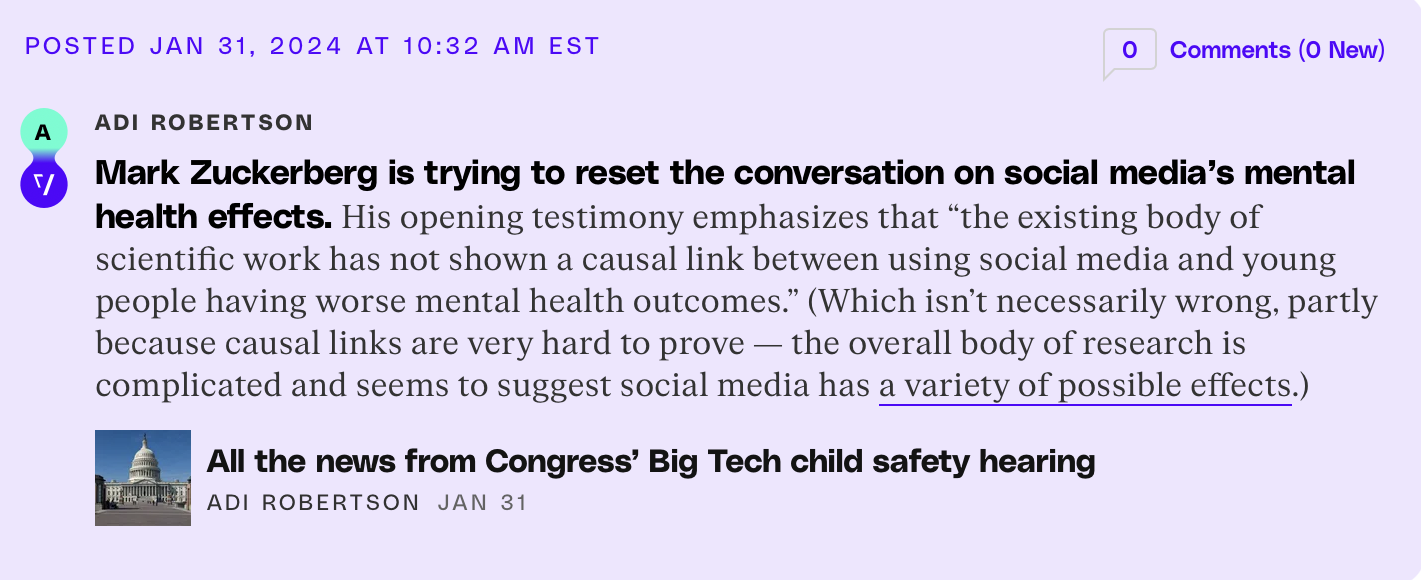
\includegraphics[scale=0.35]{./lecture_includes/facebook_quote}
\end{center}
\end{frame}



\begin{frame}{Mental health and Social Media}

\begin{itemize}
\item Unclear what he means; he may mean there is no experimental evidence
\item Very difficult to imagine a randomized experiment -- especially once the claim out there is that it is harmful, Institutional Review Boards likely wouldn't approve it
\item Quasi-experimental evidence can step in to answer important questions like this
\item Braghieri, Levy and Makarin (2022), ``Social Media and Mental Health'', \emph{American Economic Review}, 112(11): 3660-3693


\end{itemize}

\end{frame}

\begin{frame}{Overview of design and data}

\begin{itemize}
\item Authors take advantage of a clever quirk in Facebook (then ``theFacebook'') targeted different universities from 2004 to 2006
\item They found an online data source that allowed them to pin point precisely when a university was ``treated'' with theFacebook
\item They then linked that data with a longrunning health survey of college students (both before and after) in a very clever way
\item Estimated the effect of a new social media platform's presence at a university on student revealed mental health problems

\end{itemize}

\end{frame}


\begin{frame}{DID in Court}

Five elements of a strong DiD
\begin{enumerate}

\item \textbf{Bite}: \textcolor{red}{Nothing}. They cannot really show much here.  No data on Facebook usage.  They had to rely on anecdote and Facebook as a ``first mover'', but there had been Friendster and MySpace so this does weaken the paper maybe
\item \textbf{Main Results}: Very strong evidence, mostly expressed using rich survey data and questions transformed into z-scores (standard deviations)
\item \textbf{Falsifications}: \textcolor{red}{None}. Authors do not perform falsifications. Remember Miller, Johnson and Wherry looking at Medicaid's effect on Medicare eligible population?  There isn't anything like that here.
\item \textbf{Event studies}: Extremely compelling evidence and robustness across a half dozen different models
\item \textbf{Mechanism}: \textcolor{red}{Very weak in my opinion}

\end{enumerate}

\end{frame}

\begin{frame}{DiD in Court}

\begin{itemize}

\item So in many ways the strength of the project lies in a few areas:
	\begin{enumerate}
	\item Important question -- social media and youth mental health problems is a major policy question (see Zuckerberg testifying before Congress about it)
	\item Excellent research design -- difference-in-differences
	\item Meticulous data collection
	\item Data visualization is compelling
	\end{enumerate}
\item And it publishes in the premiere journal in economics, which I think shows that the research question and high quality data combined with research design can lift a paper

\end{itemize}

\end{frame}







\begin{frame}{TWFE}

\begin{equation}
Y_{icgt} = \alpha_g + \delta_t + \beta \times Facebook_{gt} + X_i \times \gamma + X_c \times \psi + \varepsilon_{icgt}
\end{equation}

\bigskip

This is a version of the regression model we looked at called "twoway fixed effects".  Somewhat complicated to dig into, so I will just say that they use it plus some other methods that are appropriate when you have several difference-in-differences events.  But the focus is on $\beta$

\end{frame}


\begin{frame}{Data on Facebook}

\begin{itemize}

\item When does Facebook appear at a school?  
	\begin{itemize}
	\item Facebook only publishes a fraction of that information
	\item They came up with a workaround
	\end{itemize}
\item The Wayback Machine has been taking almost daily photographs of every website since the Internet's beginning -- including the frontpage of ``TheFacebook''
\item Guess what was on the front page of TheFacebook \dots

\end{itemize}

\end{frame}

\begin{frame}
\begin{center}
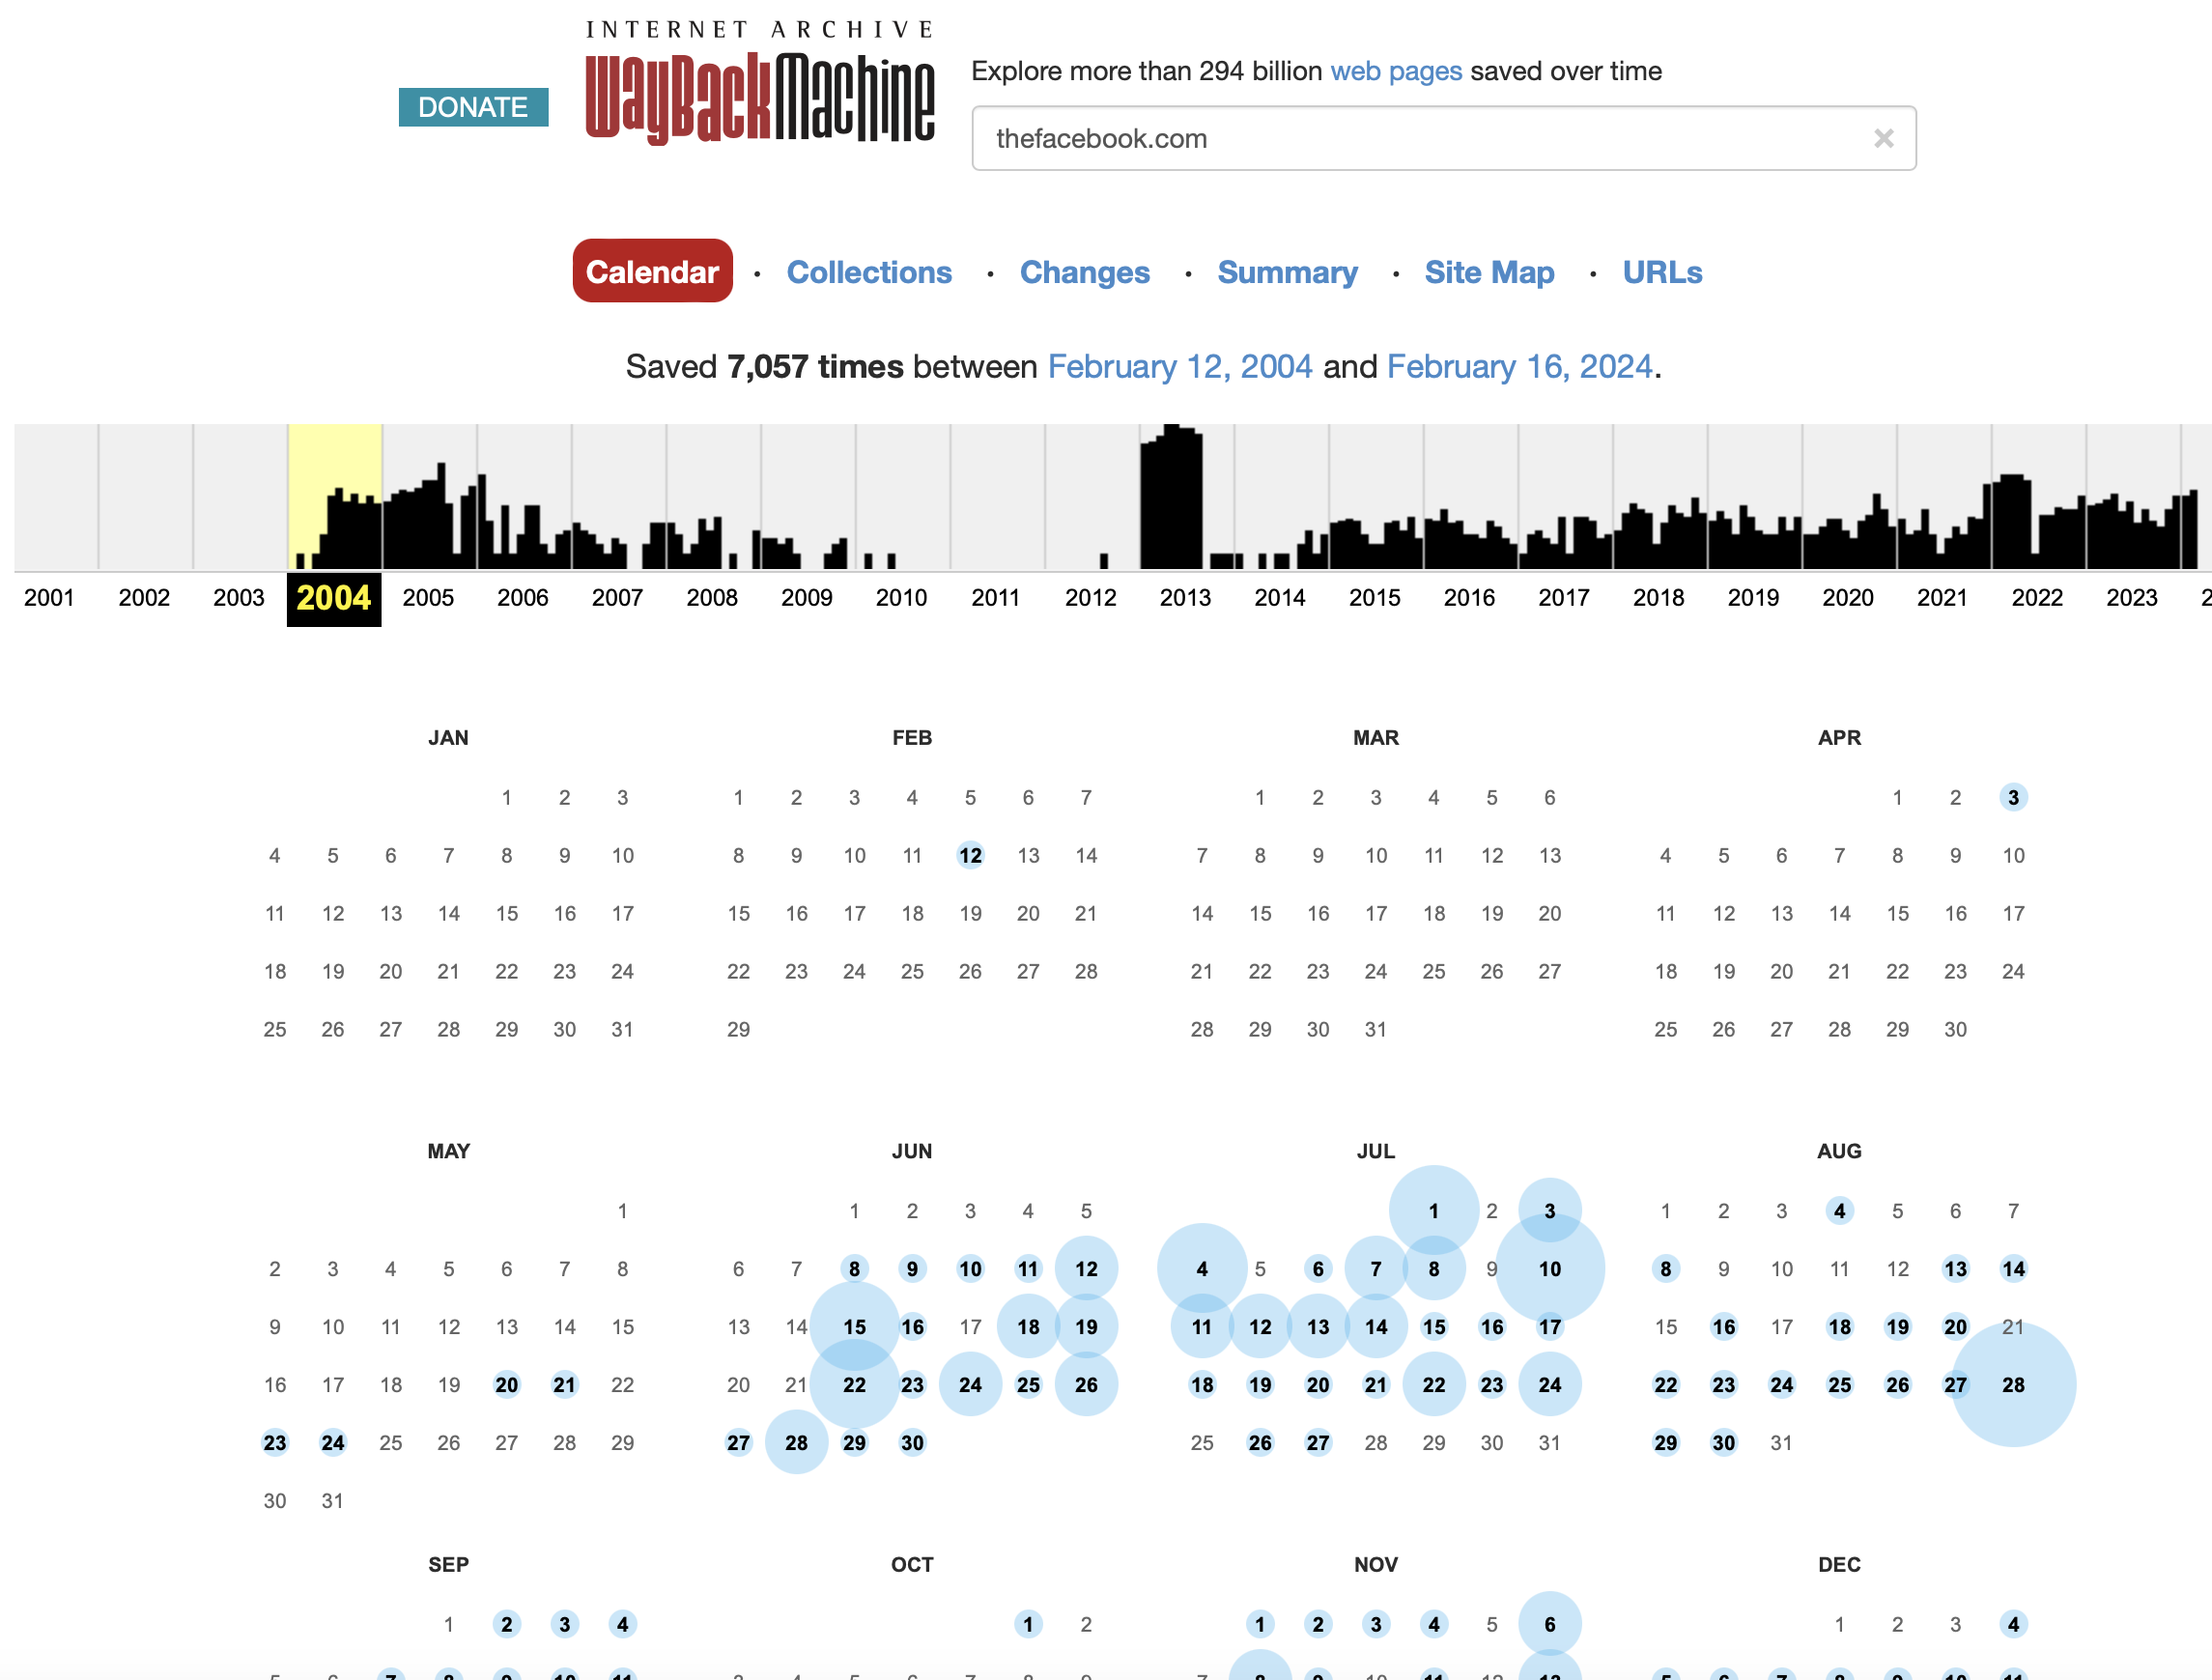
\includegraphics[scale=0.25]{./lecture_includes/wayback1}
\end{center}
\end{frame}

\begin{frame}
\begin{center}
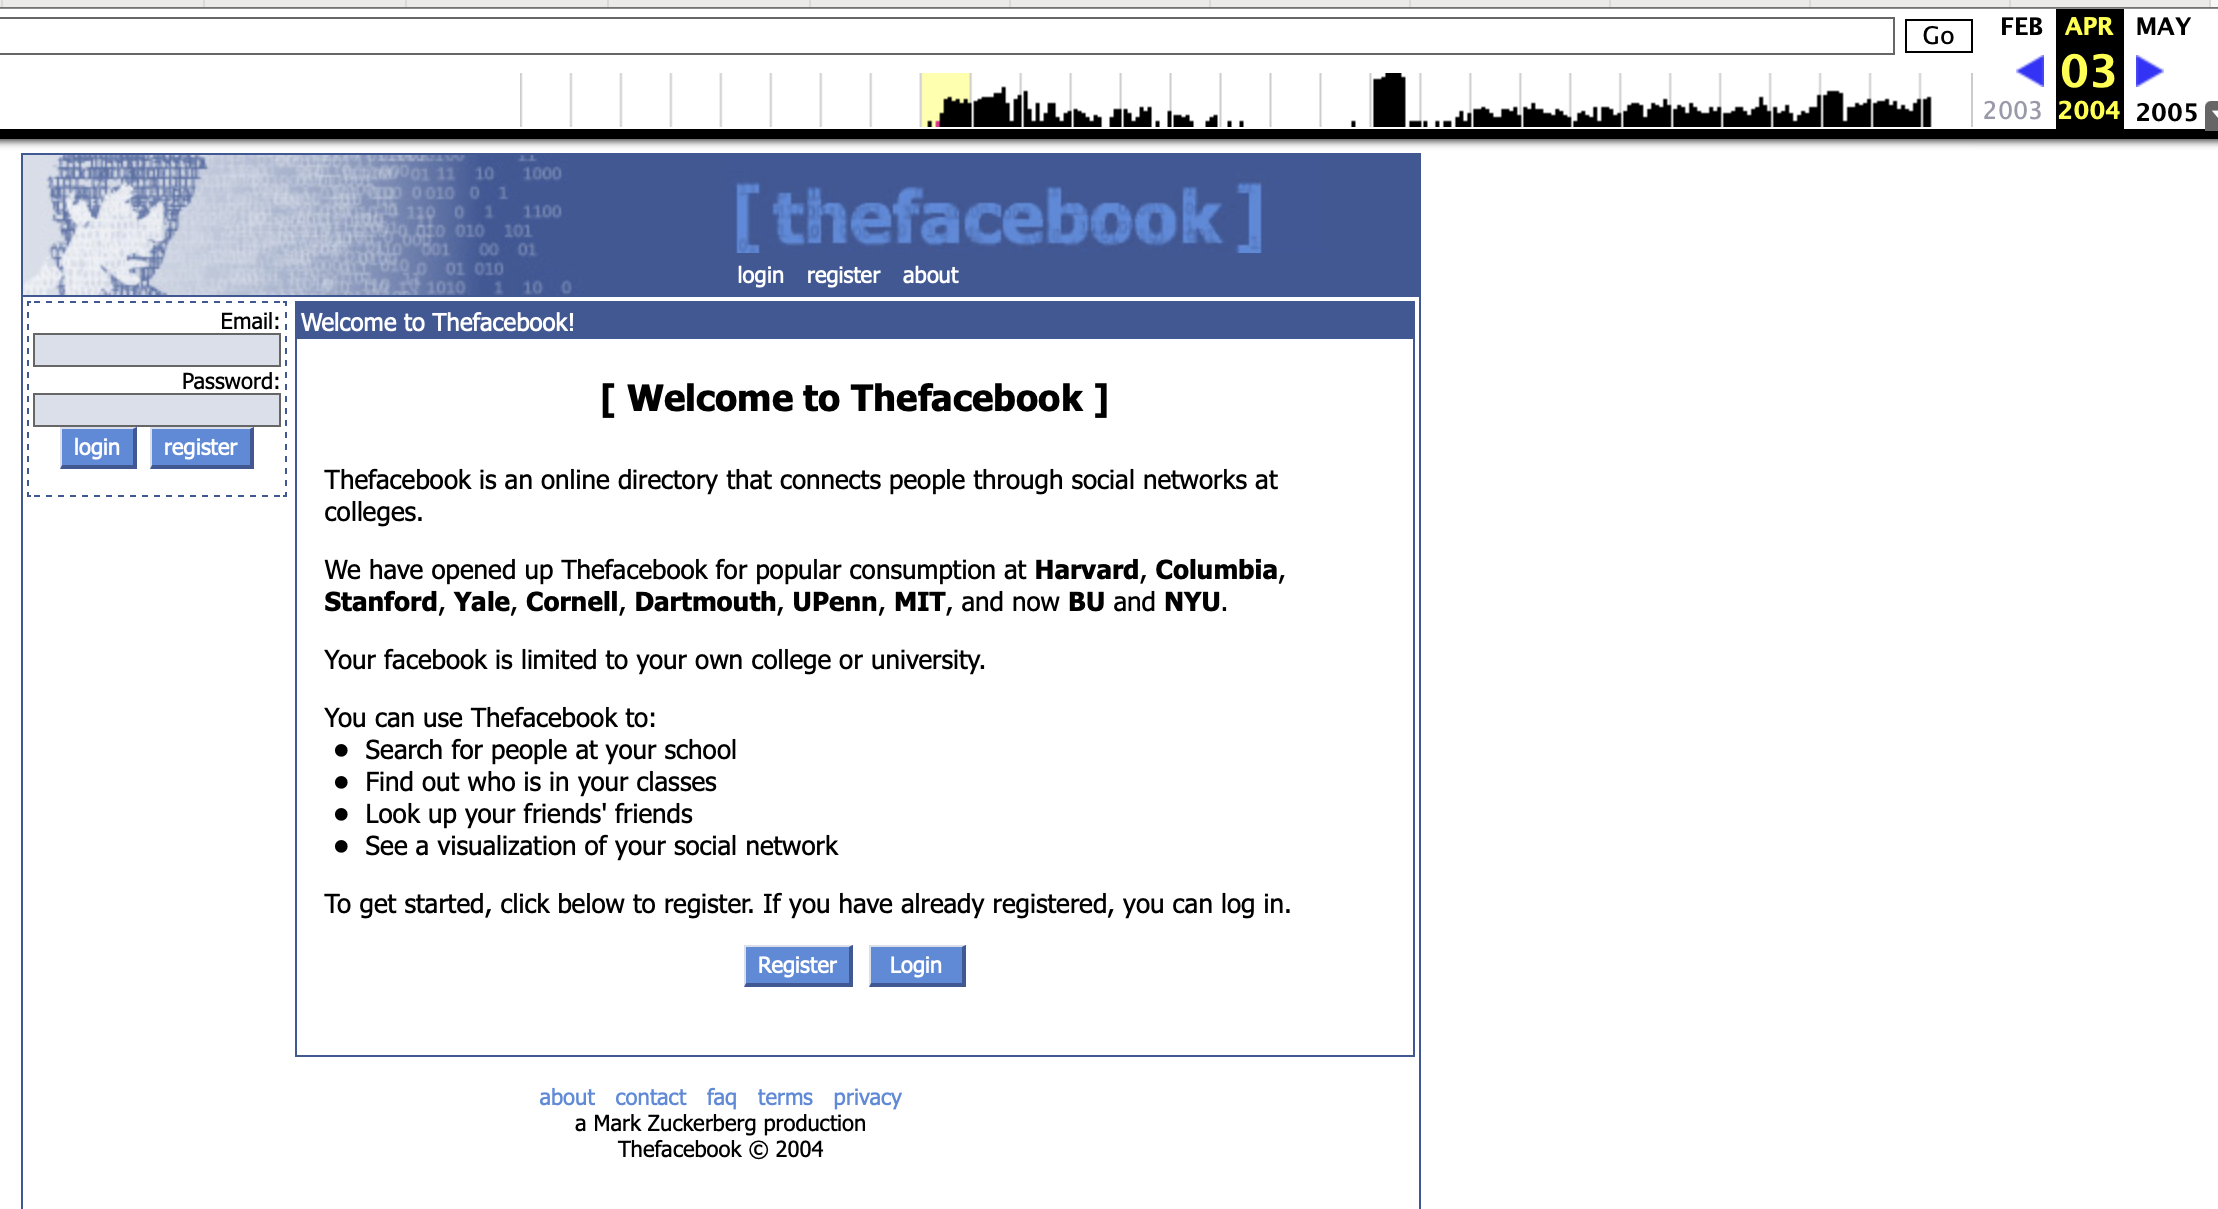
\includegraphics[scale=0.35]{./lecture_includes/wayback2}
\end{center}
\end{frame}

\begin{frame}
\begin{center}
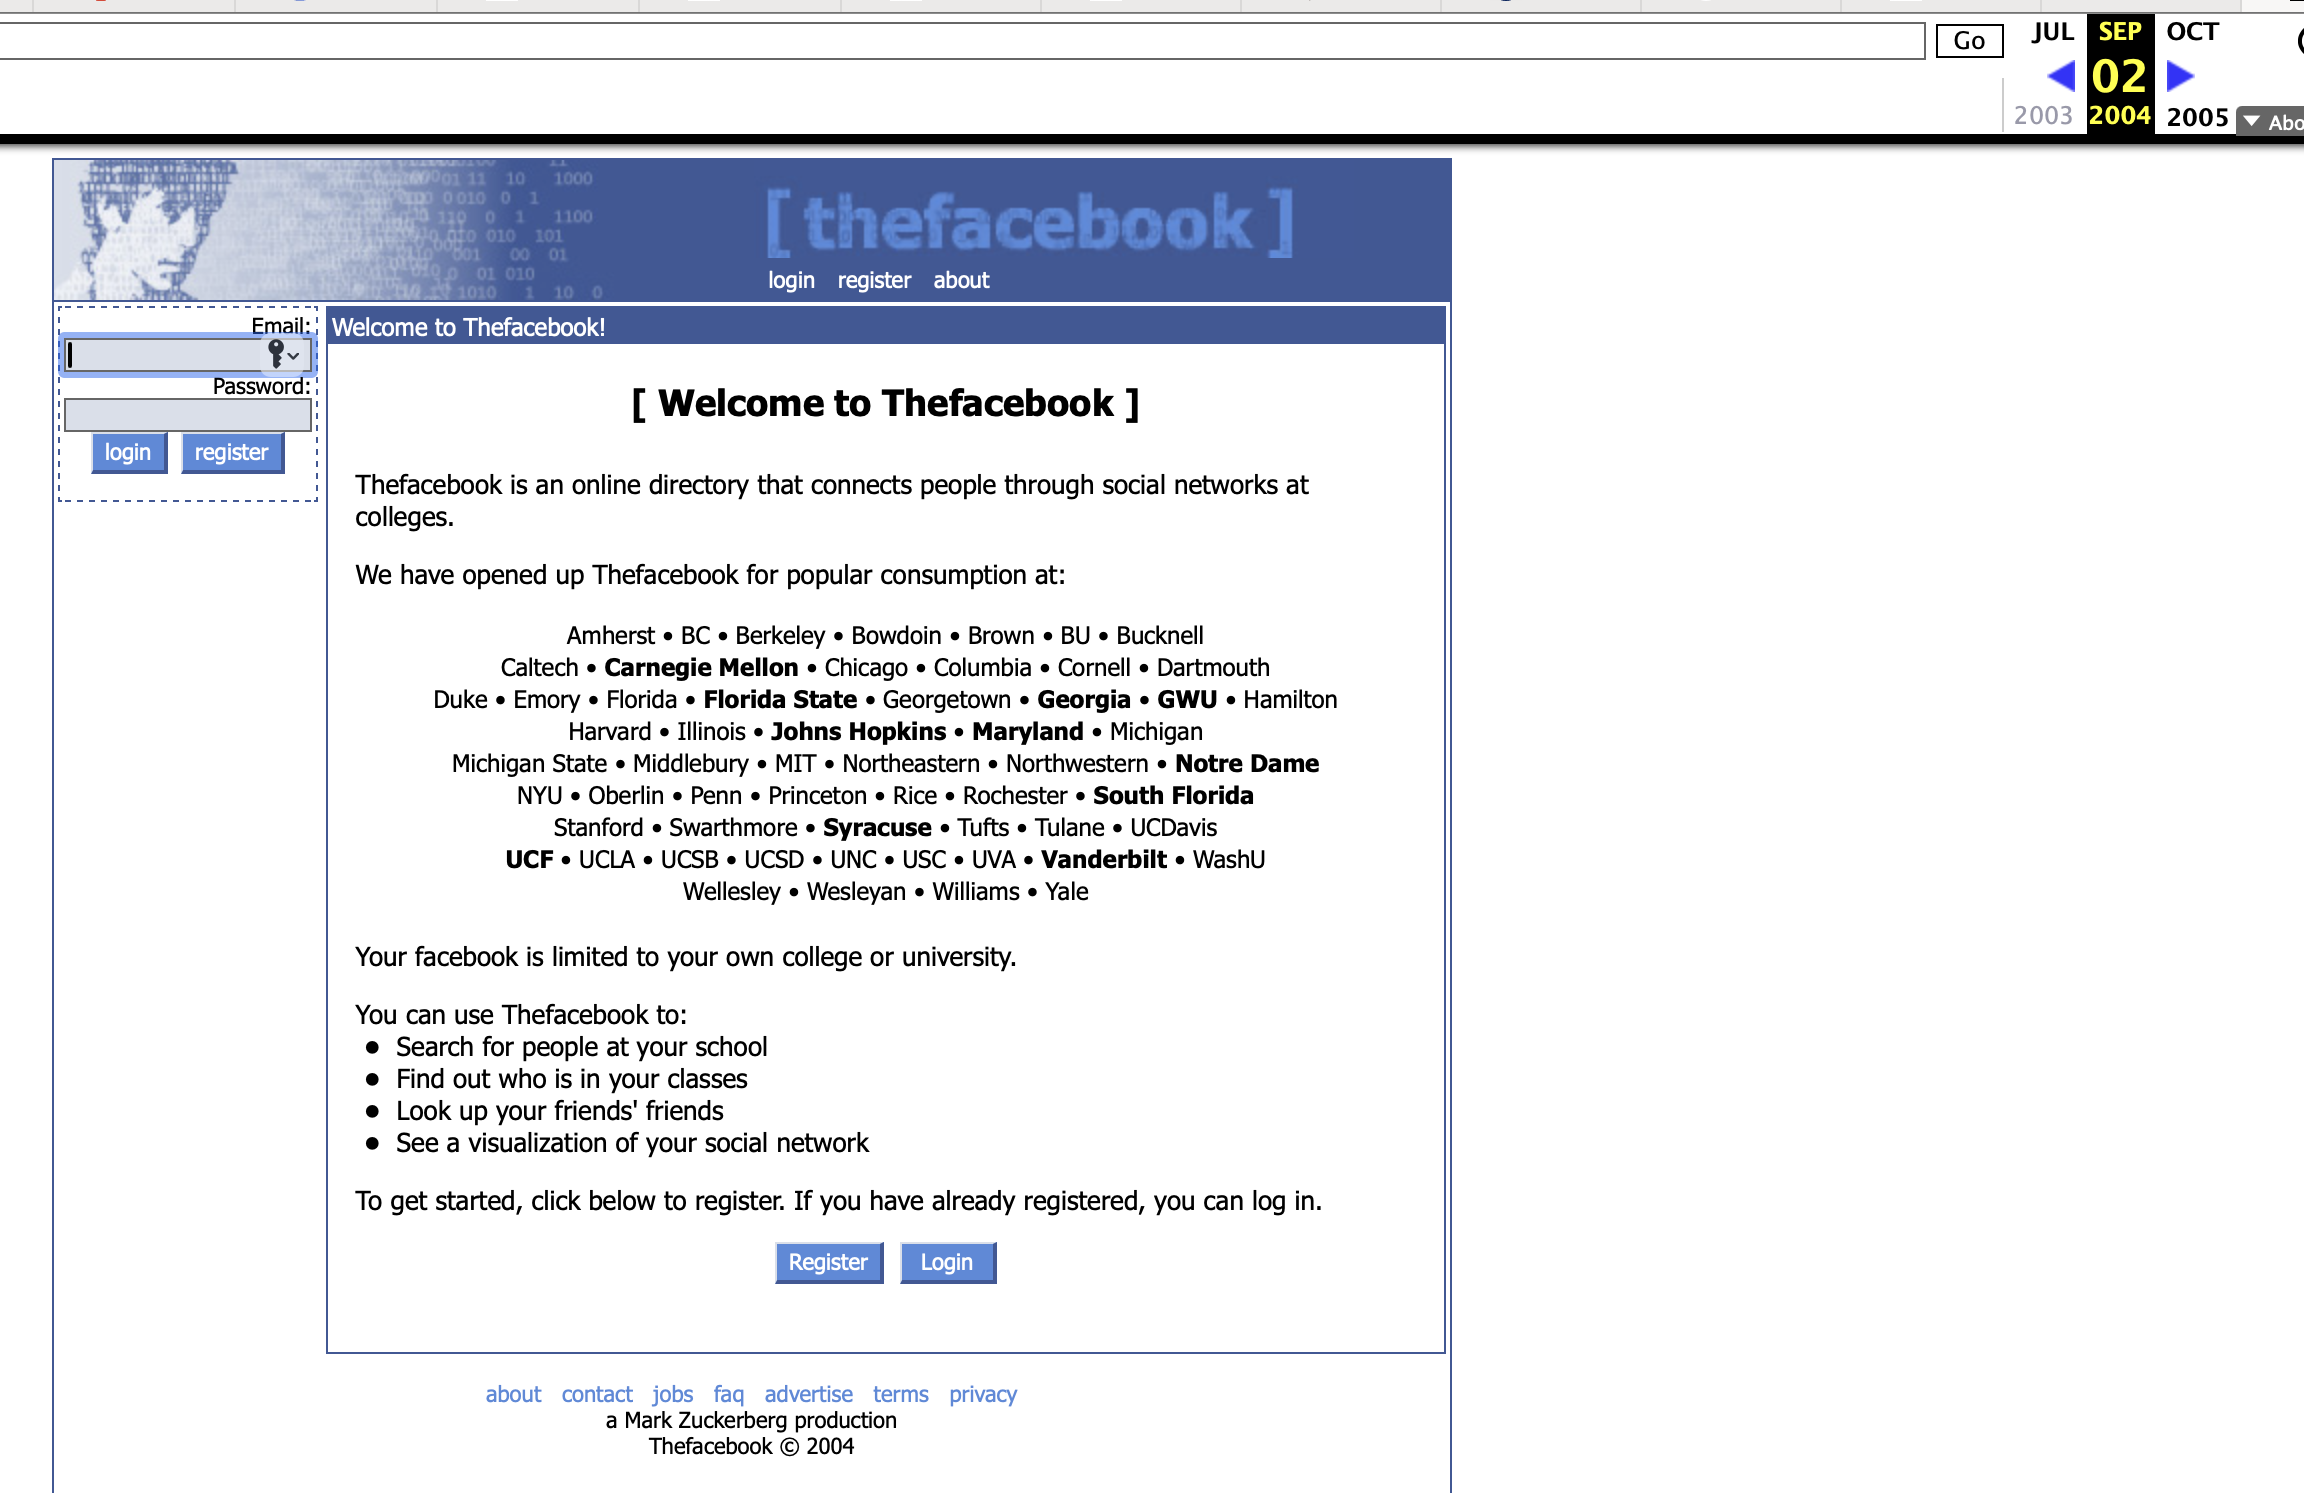
\includegraphics[scale=0.25]{./lecture_includes/wayback3}
\end{center}
\end{frame}

\begin{frame}
\begin{center}
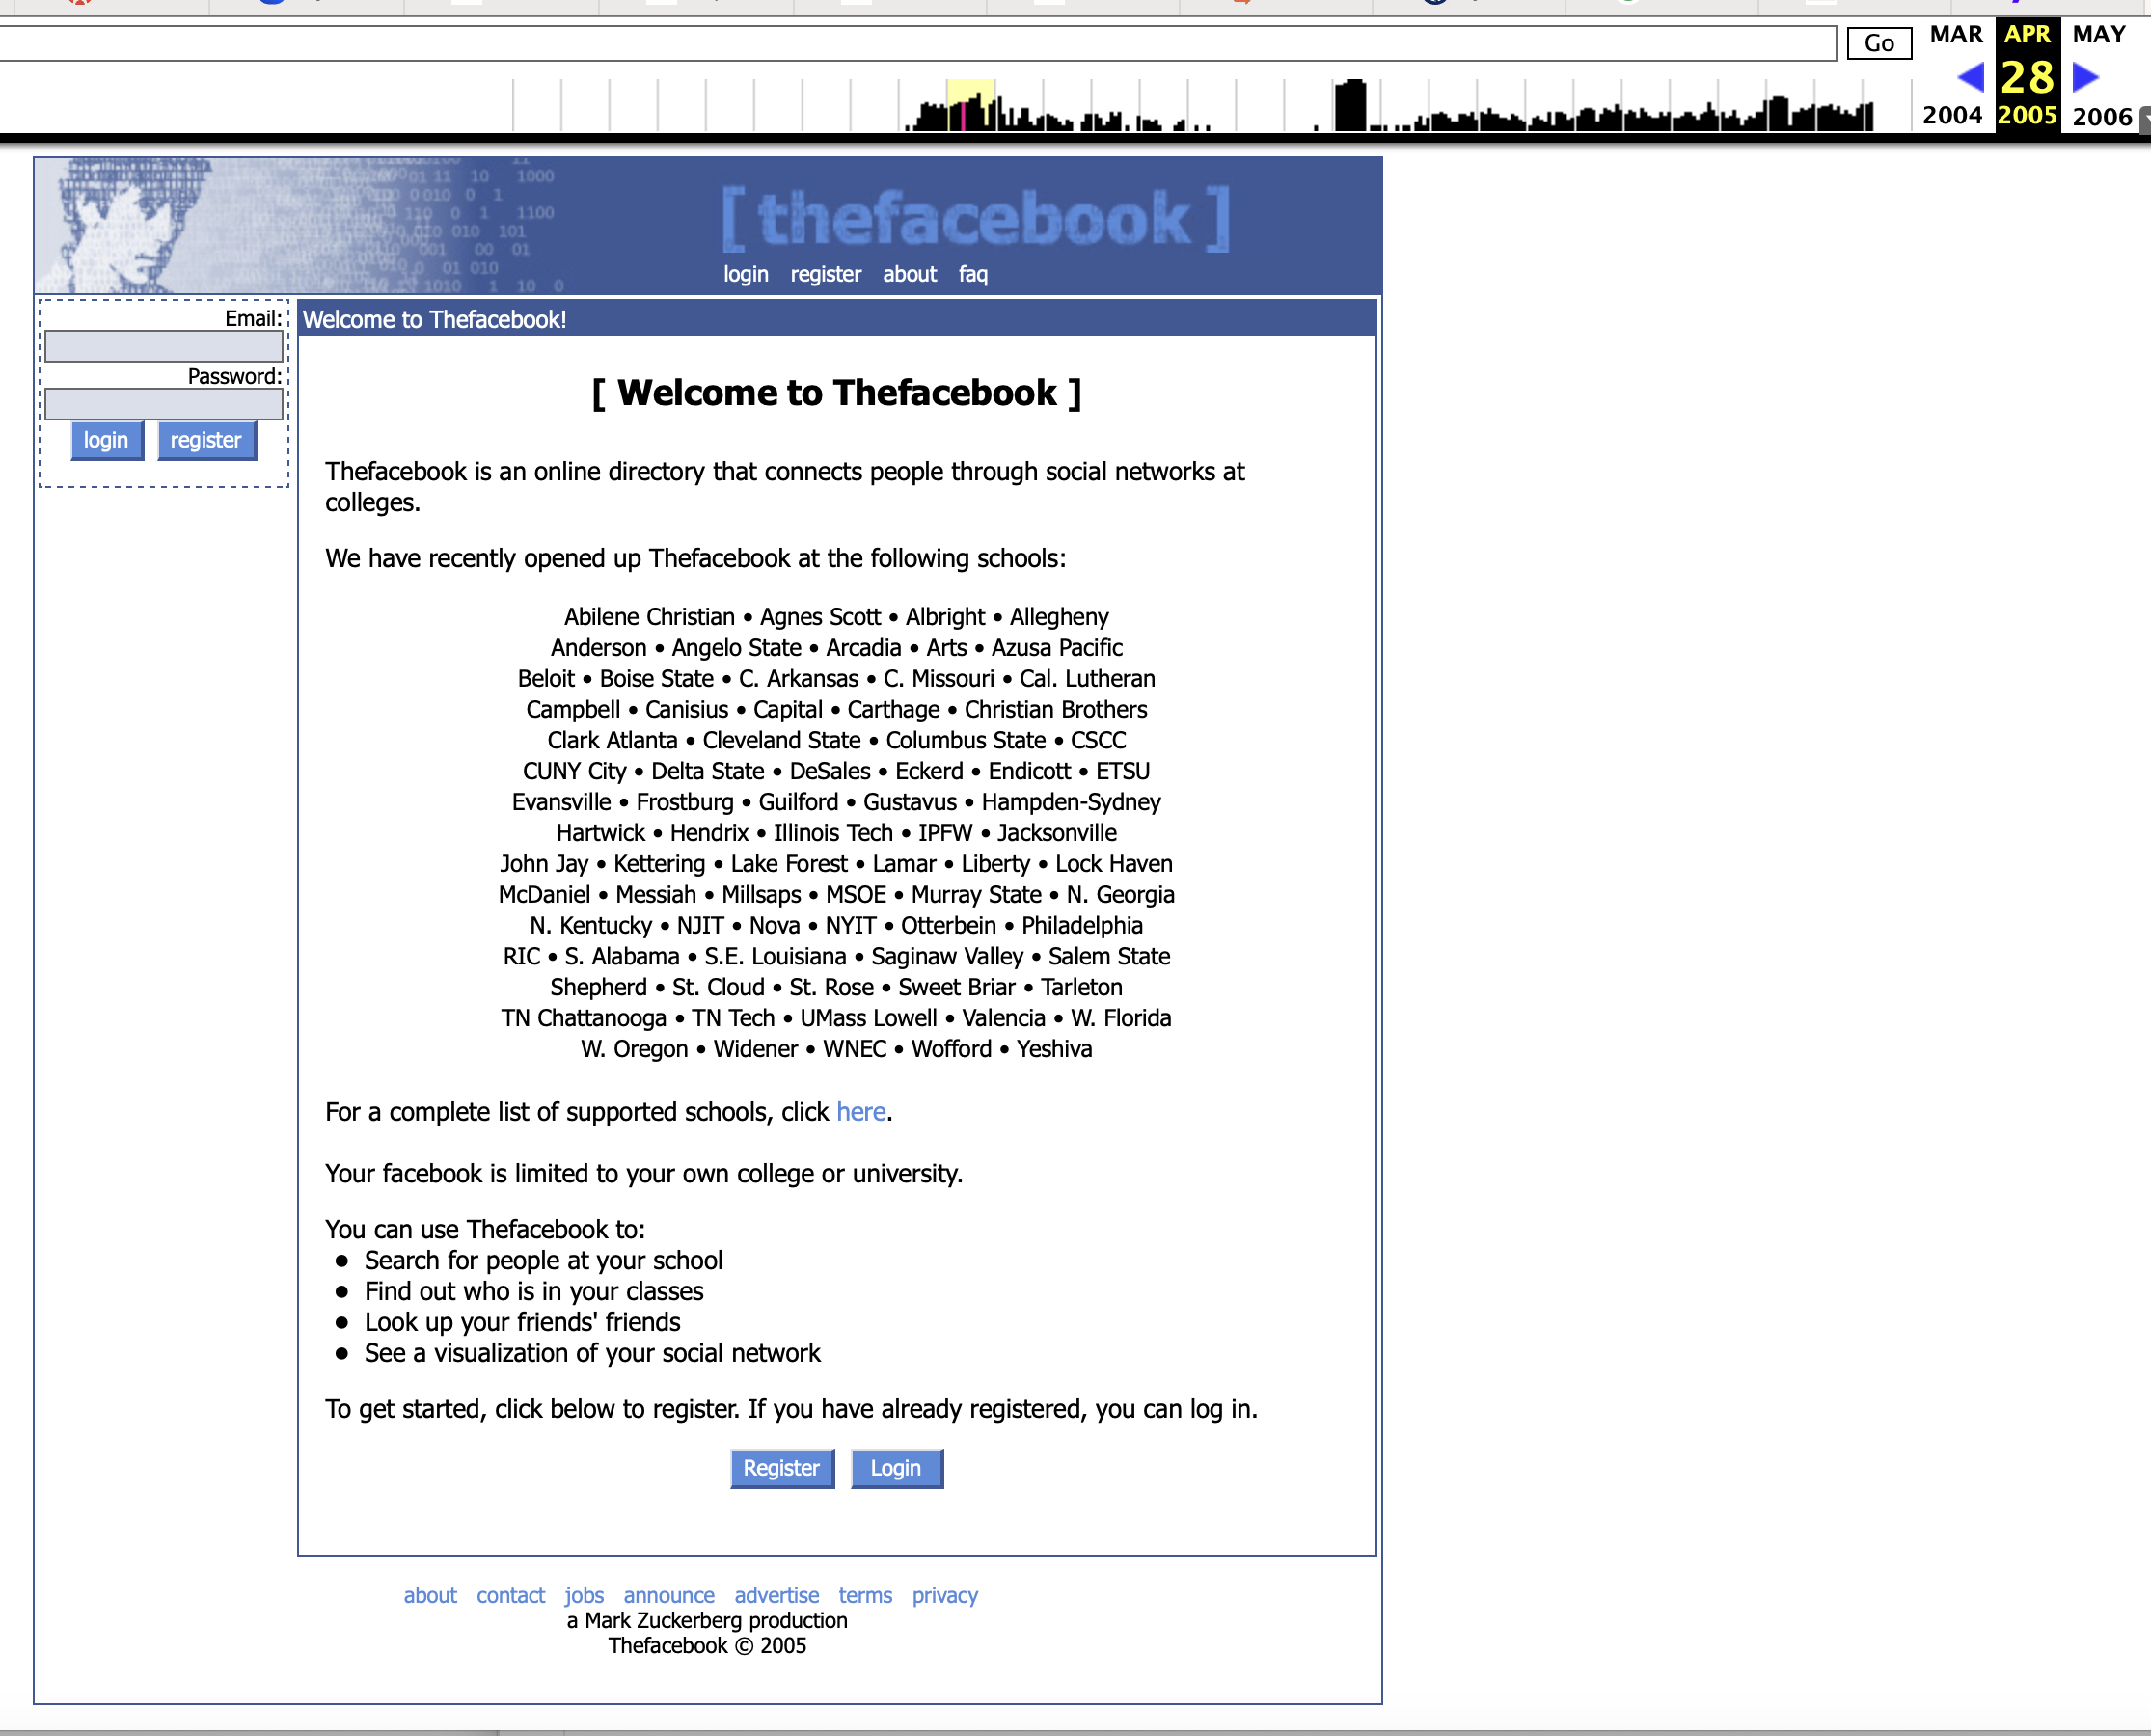
\includegraphics[scale=0.25]{./lecture_includes/wayback4}
\end{center}
\end{frame}

\begin{frame}{Timing Dates}

\begin{itemize}
\item They went through three years of daily screenshots on Wayback machine to find when a school appeared on the front page
\item The first time Agnes Scott, or Covenant, appears on the front page, the authors mark that as the date when the school got Facebook
\item But now they need information on mental health outcomes
\item They find it with an old long running repeated cross section survey of college students
\end{itemize}

\end{frame}

\begin{frame}{NCHA survey by ACHA}

\begin{quote}
Our second main data source consists of more than 430,000 responses to the NCHA survey, a survey administered to college students on a semi-annual basis by the American College Health Association (ACHA). The NCHA survey was developed in 1998 by a team of college health professionals with the purpose of obtaining information from college students about their mental and physical health. Specifically, the NCHA survey inquires about demographics, physical health, \textbf{mental health}, alcohol and drug use, sexual behaviors, and perceptions of these behaviors among one’s peers.
\end{quote}

\end{frame}

\begin{frame}{No evidence of bite}

\begin{quote}
The NCHA survey does not include any questions on social media use; therefore, it is not possible for us to determine whether a particular survey respondent had a Facebook account.
\end{quote}

\bigskip

This is probably the problem in any study in which your treatment is more or less the first of its kind -- most likely the standard surveys have not yet incorporated the questions into their surveys

\end{frame}

\begin{frame}{Linking Facebook data with NCHA data}

\begin{quote}
In order to protect the privacy of the institutions that participate in the NCHA survey while still allowing us to carry out the analysis, the ACHA kindly agreed to provide us with a customized dataset that includes a variable indicating the semester in which Facebook was rolled out at each college. Specifically, the ACHA adopted the following procedure: (i) merge our dataset containing the Facebook introduction dates to the NCHA dataset; (ii) add a variable listing the semester in which Facebook was rolled out at each college;15 (iii) strip away any information that could allow us to identify colleges (including the specific date in which Facebook was introduced at each college).
\end{quote}

\end{frame}

\begin{frame}{Basic facts about early and late adopters}

\begin{itemize}
\item Colleges in earlier Facebook expansion groups are more selective in terms of test scores, larger, more likely to be on the East Coast, and have more residential undergraduate programs than colleges in later Facebook expansion groups. 

\item Colleges in earlier Facebook expansion groups enroll students from relatively more advantaged economic backgrounds. 

\item Students in colleges that received Facebook relatively earlier have worse baseline mental health outcomes than students attending colleges in later Facebook expansion groups. 

%The baseline differences across Facebook expansion groups may lead one to wonder about the plausibility of the parallel trends assumption in this setting; we address concerns related to parallel trends in Section III.

\end{itemize}

\end{frame}

\begin{frame}{Measurement}

\begin{itemize}
\item The survey data is very rich with a lot of questions about mental health with different scales
\item They create their own combinations of these questions into aggregate indices -- ``index of poor mental health'' where higher numbers mean worse mental health
\item Each outcome survey question is normalized into what is called a ``z-score'' which is interpreted as a fraction of a standard deviation
\item Estimates are ATT parameters -- average effect of Facebook on students at schools that got Facebook
\end{itemize}

\end{frame}


\begin{frame}
\begin{center}
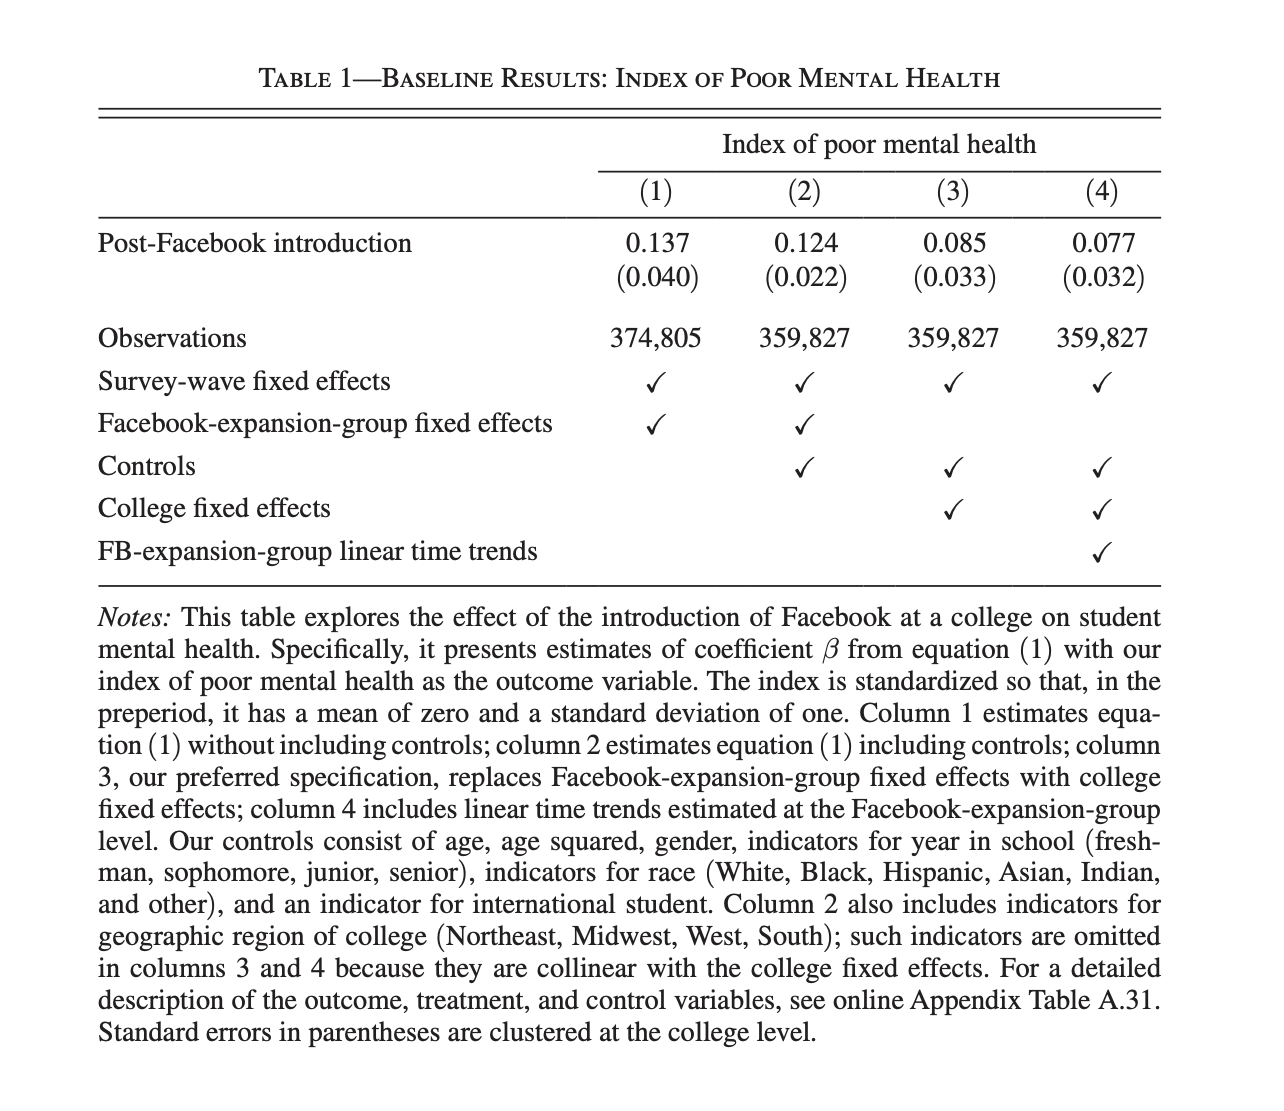
\includegraphics[scale=0.35]{./lecture_includes/facebook_1}
\end{center}
\end{frame}

\begin{frame}
\begin{center}
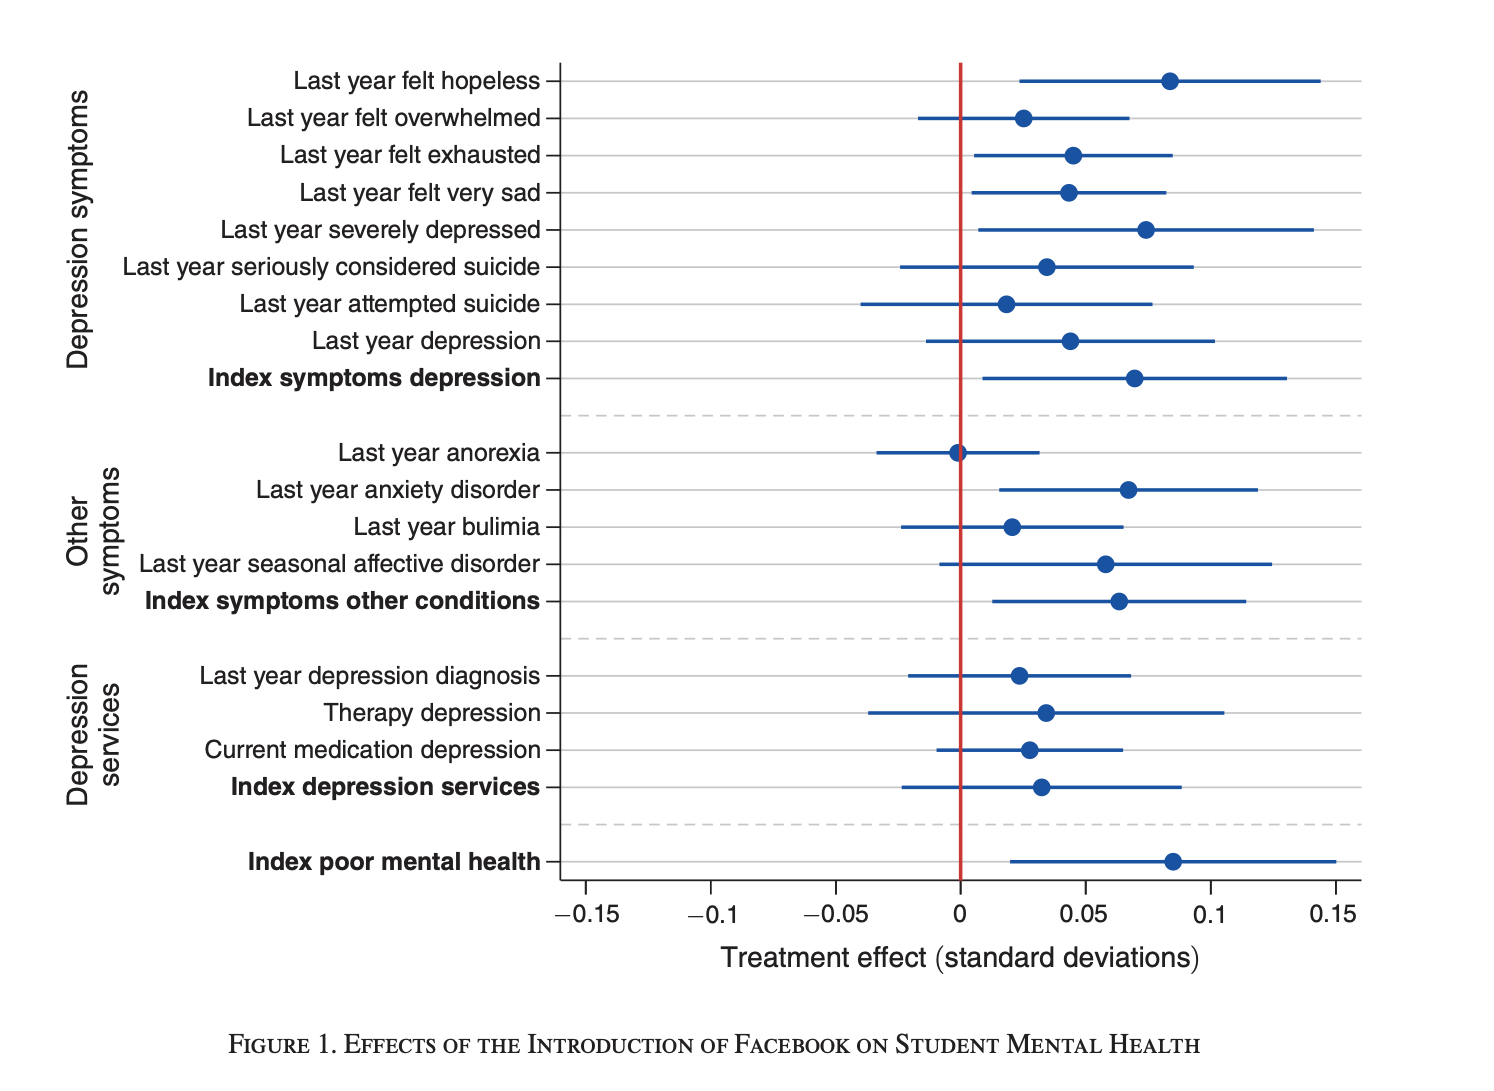
\includegraphics[scale=0.35]{./lecture_includes/facebook_2}
\end{center}
\end{frame}

\begin{frame}
\begin{center}
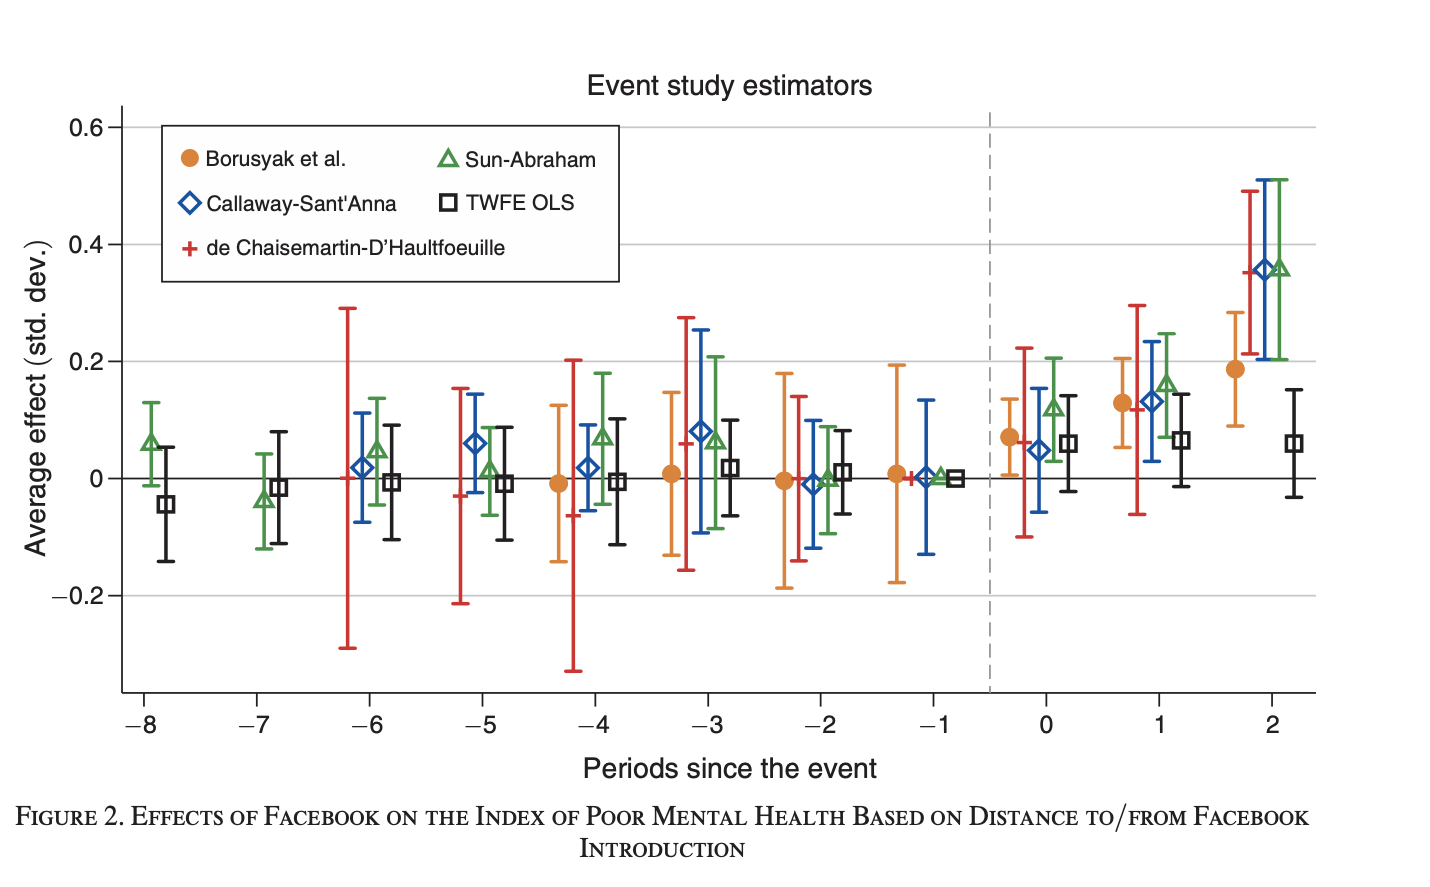
\includegraphics[scale=0.35]{./lecture_includes/facebook_3}
\end{center}
\end{frame}

\begin{frame}
\begin{center}
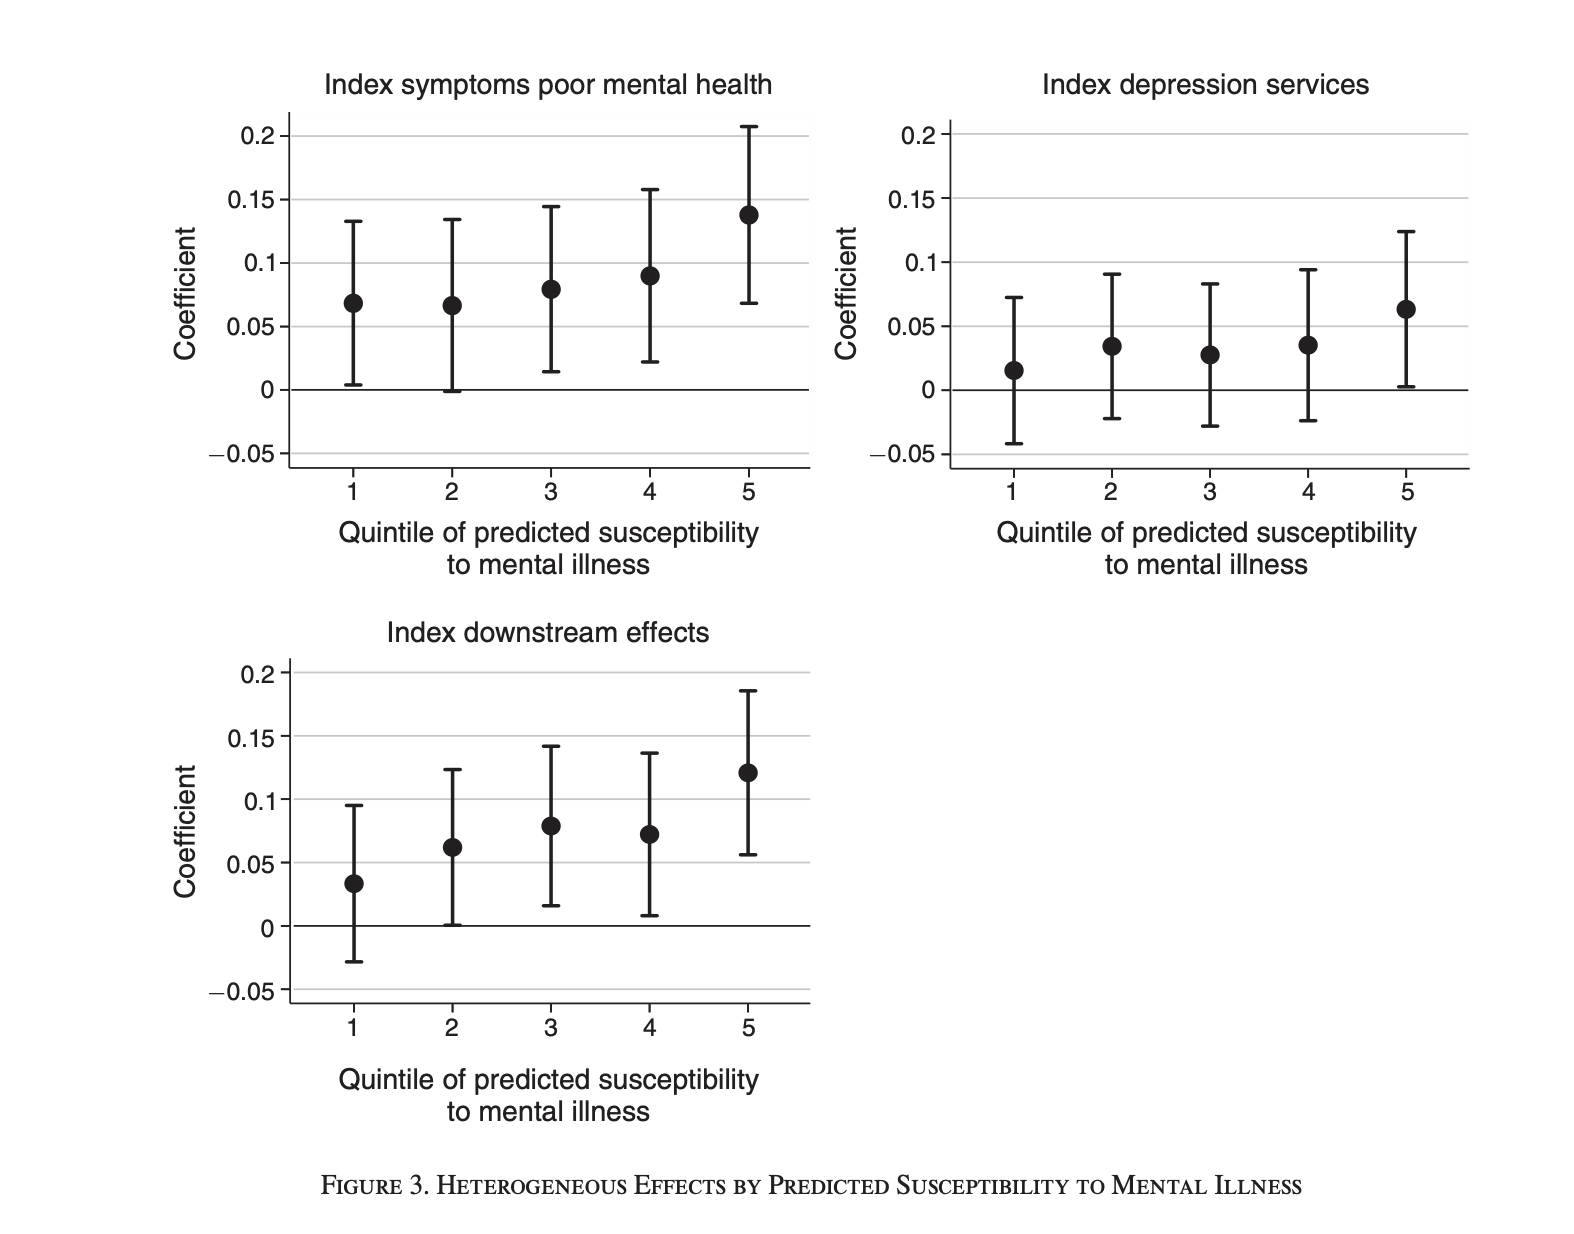
\includegraphics[scale=0.35]{./lecture_includes/facebook_4}
\end{center}
\end{frame}

\begin{frame}
\begin{center}
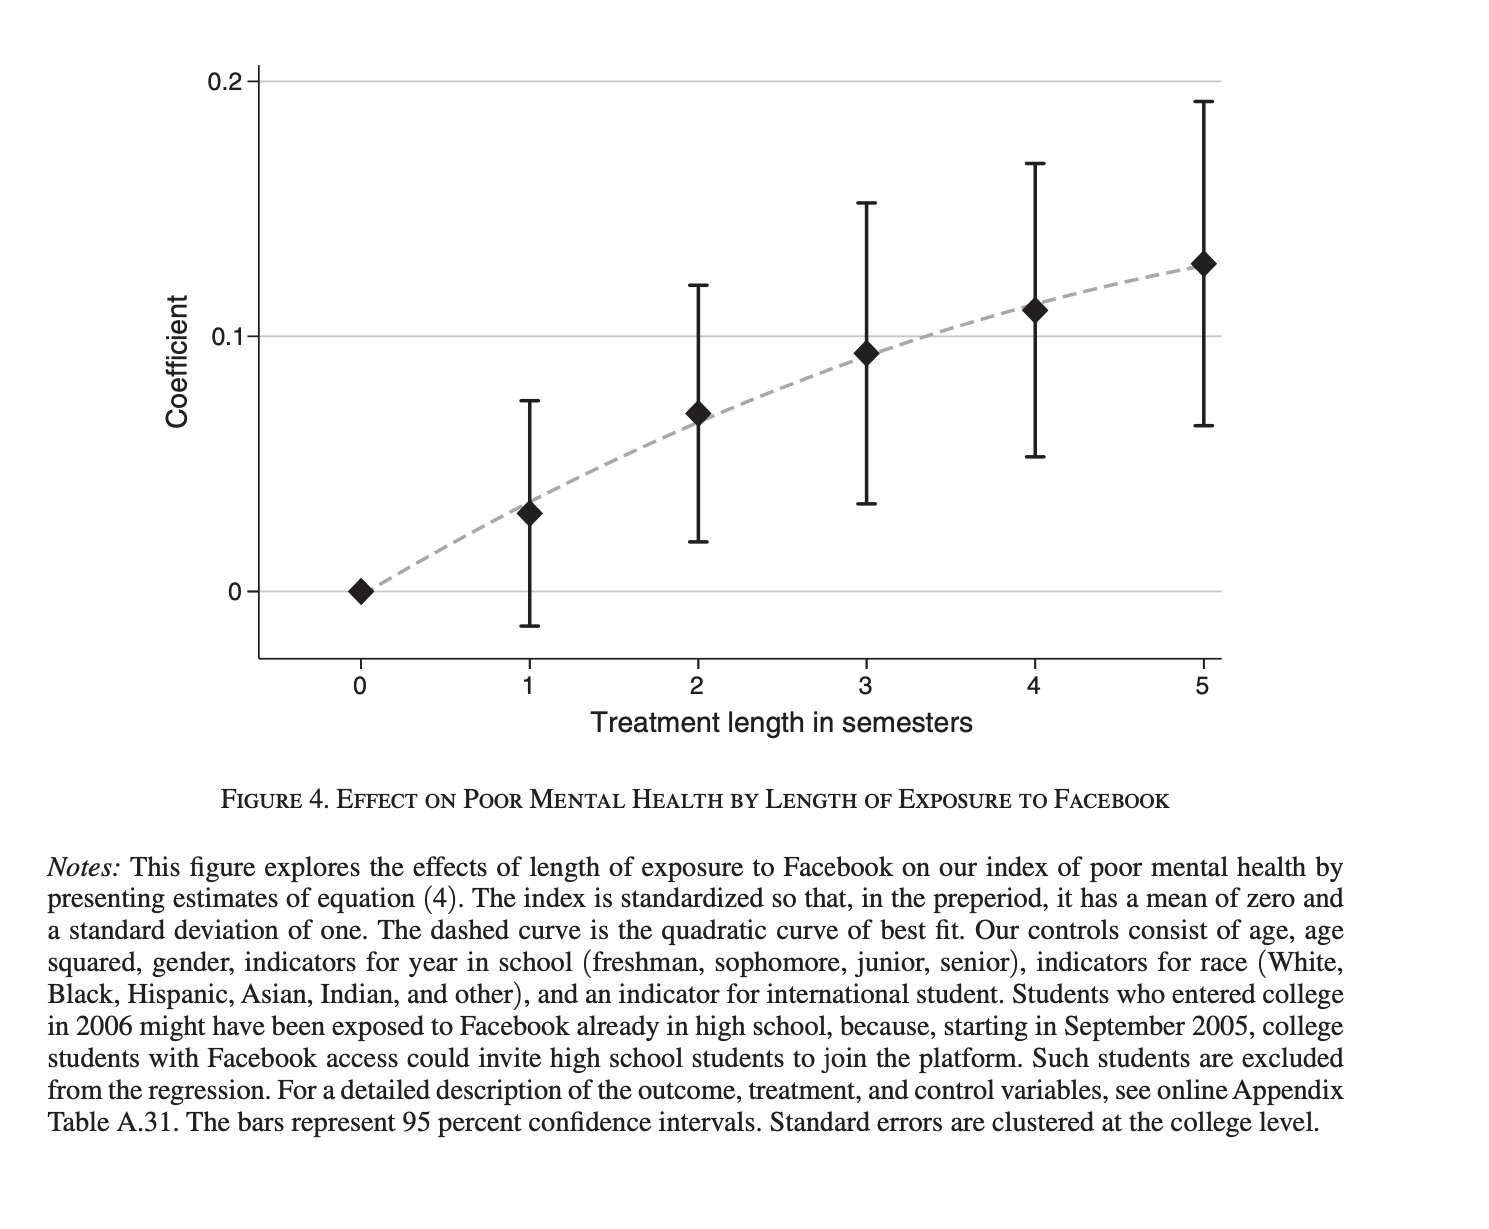
\includegraphics[scale=0.35]{./lecture_includes/facebook_5}
\end{center}
\end{frame}

\begin{frame}
\begin{center}
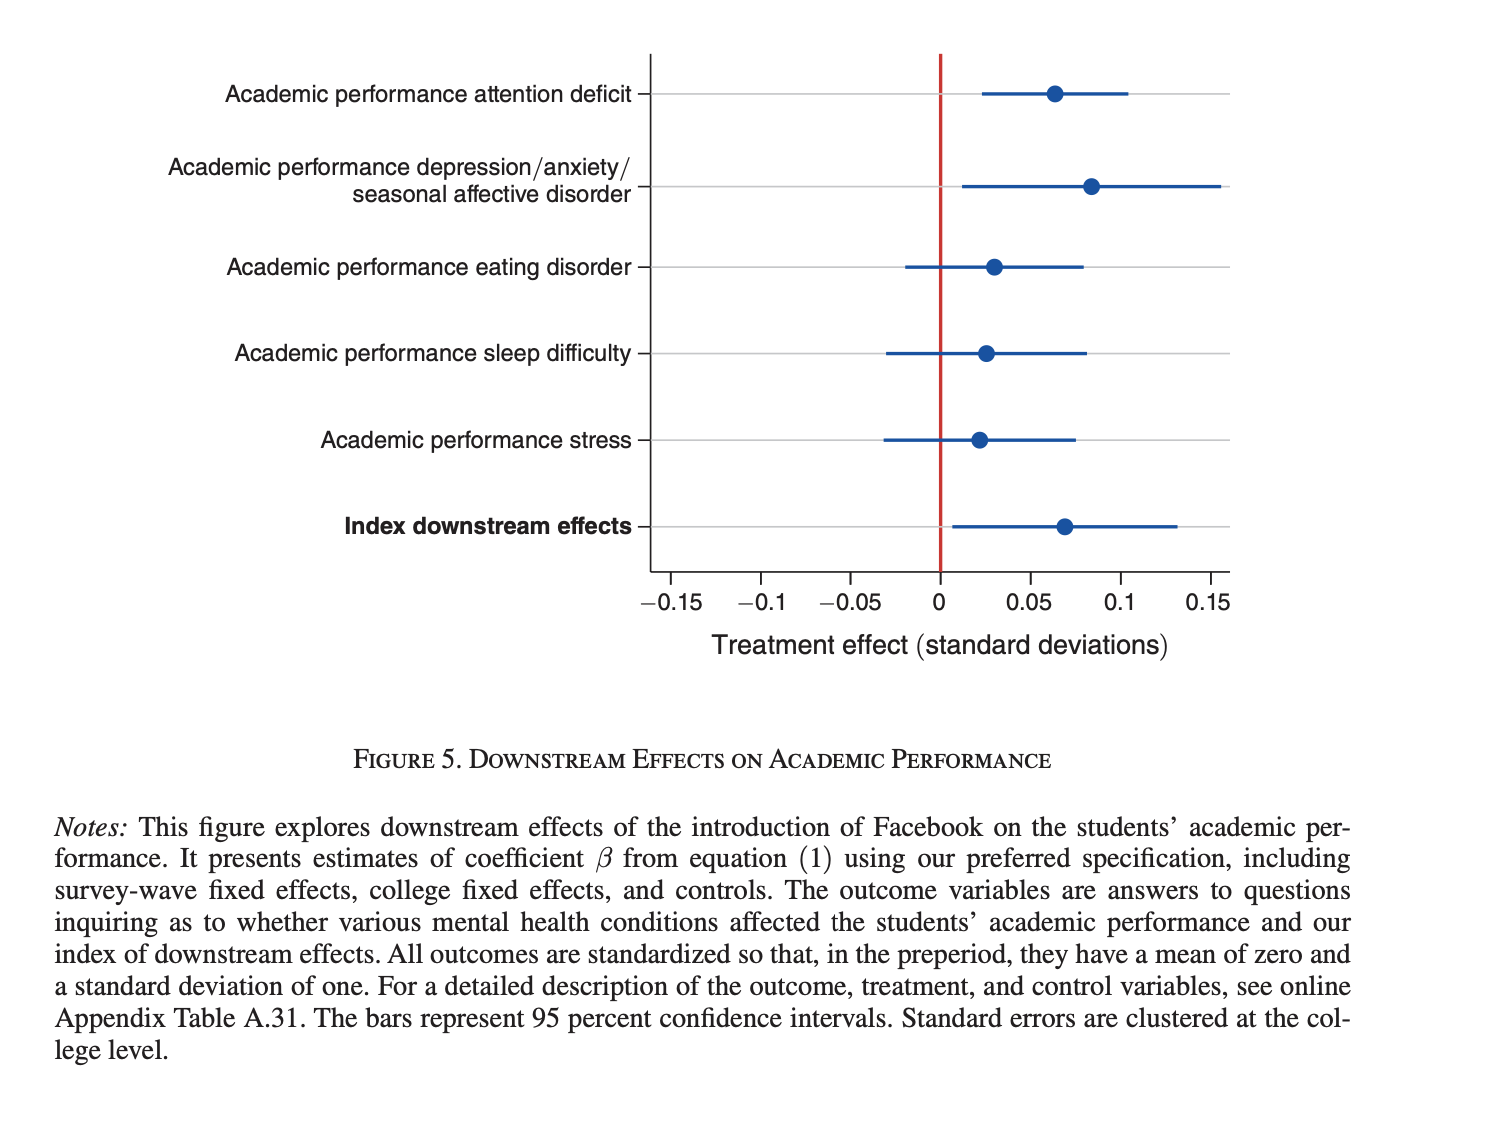
\includegraphics[scale=0.35]{./lecture_includes/facebook_6}
\end{center}
\end{frame}

\begin{frame}
\begin{center}
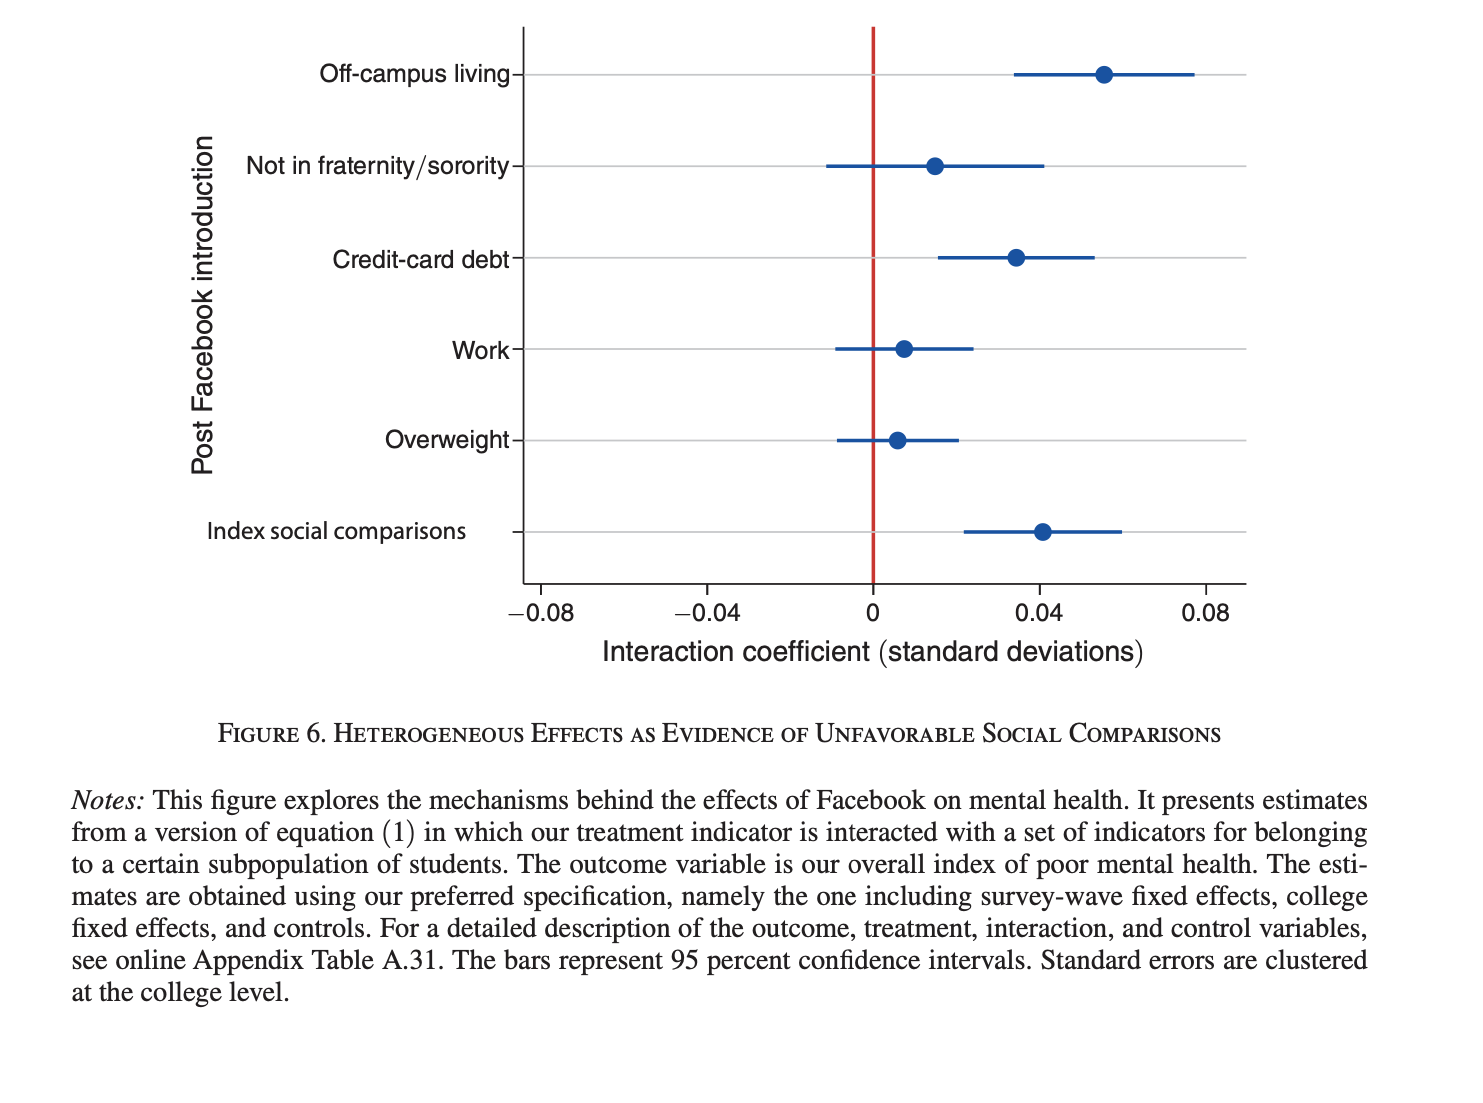
\includegraphics[scale=0.35]{./lecture_includes/facebook_7}
\end{center}
\end{frame}

\begin{frame}{Questions and Comments}

\begin{itemize}
\item Mark Zuckerberg quote: ``the existing body of scientific work has not shown a causal link between using social media and young people having worse mental health outcomes'' -- What is your reaction to his claim?
\item What is your reaction to this study's evidence?  
\item Which parts of this study do you think is more memorable and more convincing and why?
\item How might you replicate this study yourself?

\end{itemize}

\end{frame}


\subsection{ChatBot Rollout}

\begin{frame}{Working Paper on ChatBot}
\begin{center}
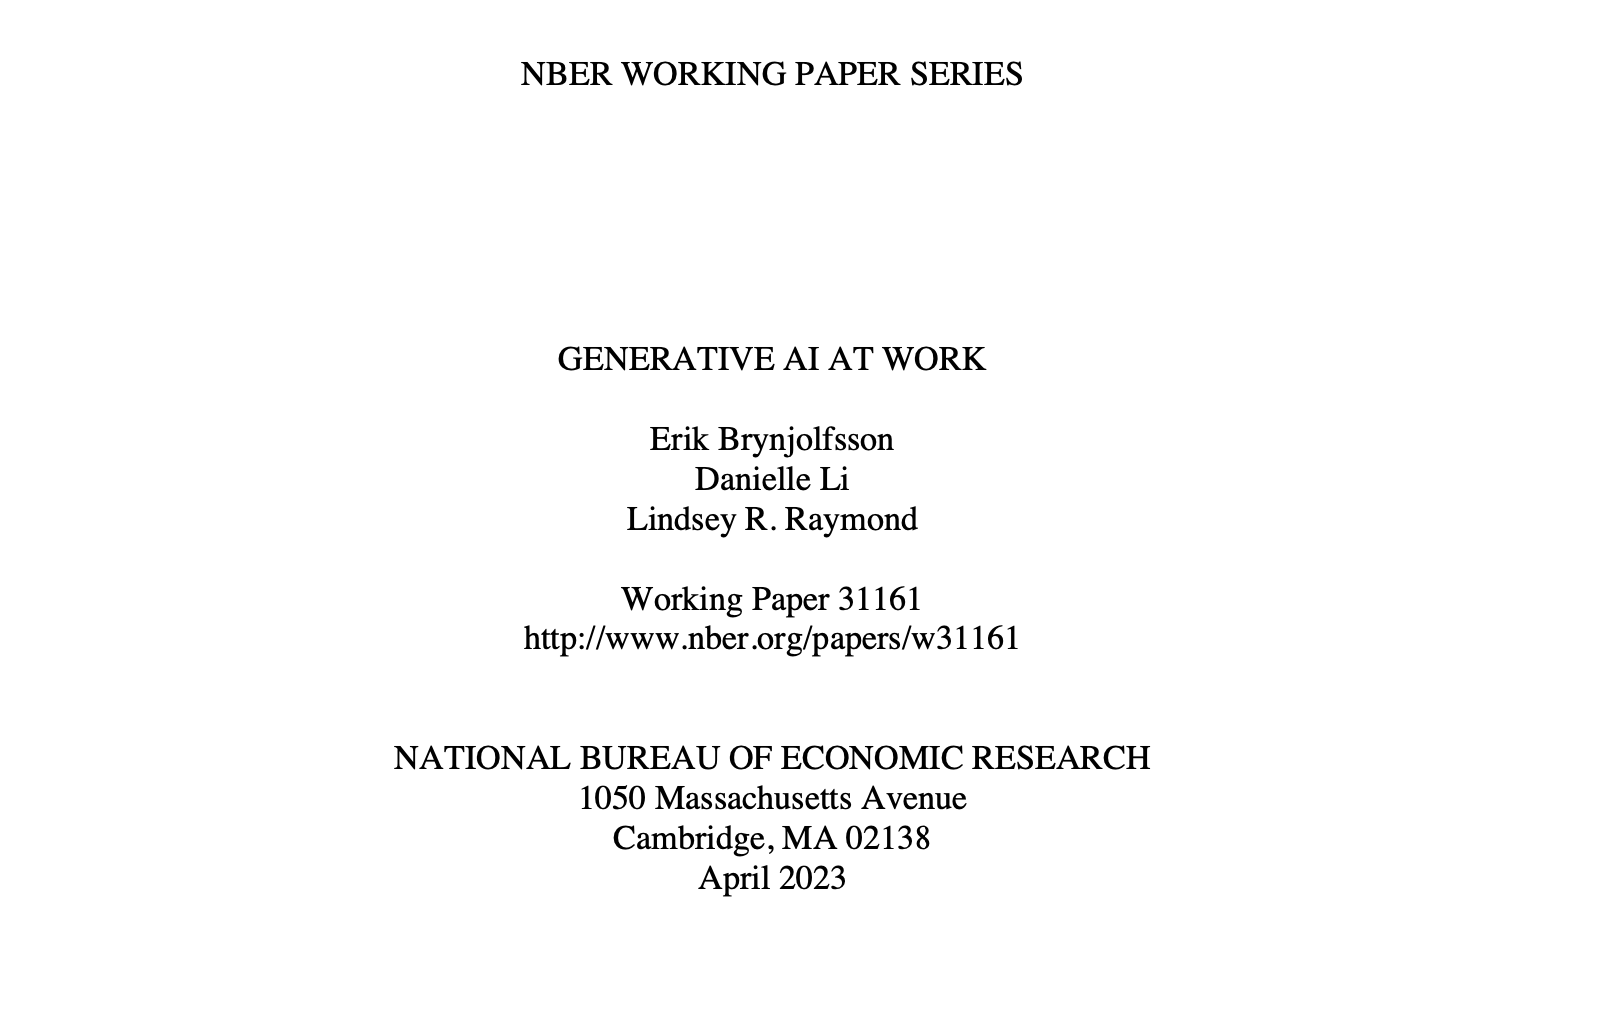
\includegraphics[scale=0.35]{./lecture_includes/brynn}
\end{center}
\end{frame}



\begin{frame}{Chatbots and Workers}

\begin{itemize}

\item An unnamed firm released gradually a generative AI-based conversational assistant chatbot to its  5,179 customer support agents 
\item These chatbots provided assistance in handling complaints
\item Very stressful job as the only time customers reached out was when they were very upset
\item It isn't a randomized experiment so they're going to estimate the effect of the adoption of the chatbot using difference-in-differences

\end{itemize}

\end{frame}

\begin{frame}{Outcomes and Pictures}

\begin{itemize}

\item Main focus is on various measures of customer support agents handling of calls, which is the proxy for their productivity
\item But they also focus on high and low skill workers (heterogeneity like before)
\item Authors are going to present evidence almost entirely using event study graphs
\item They also present regression tables, but the event study graphs are very powerful

\end{itemize}

\end{frame}




\begin{frame}{Example of ChatBot}
\begin{center}
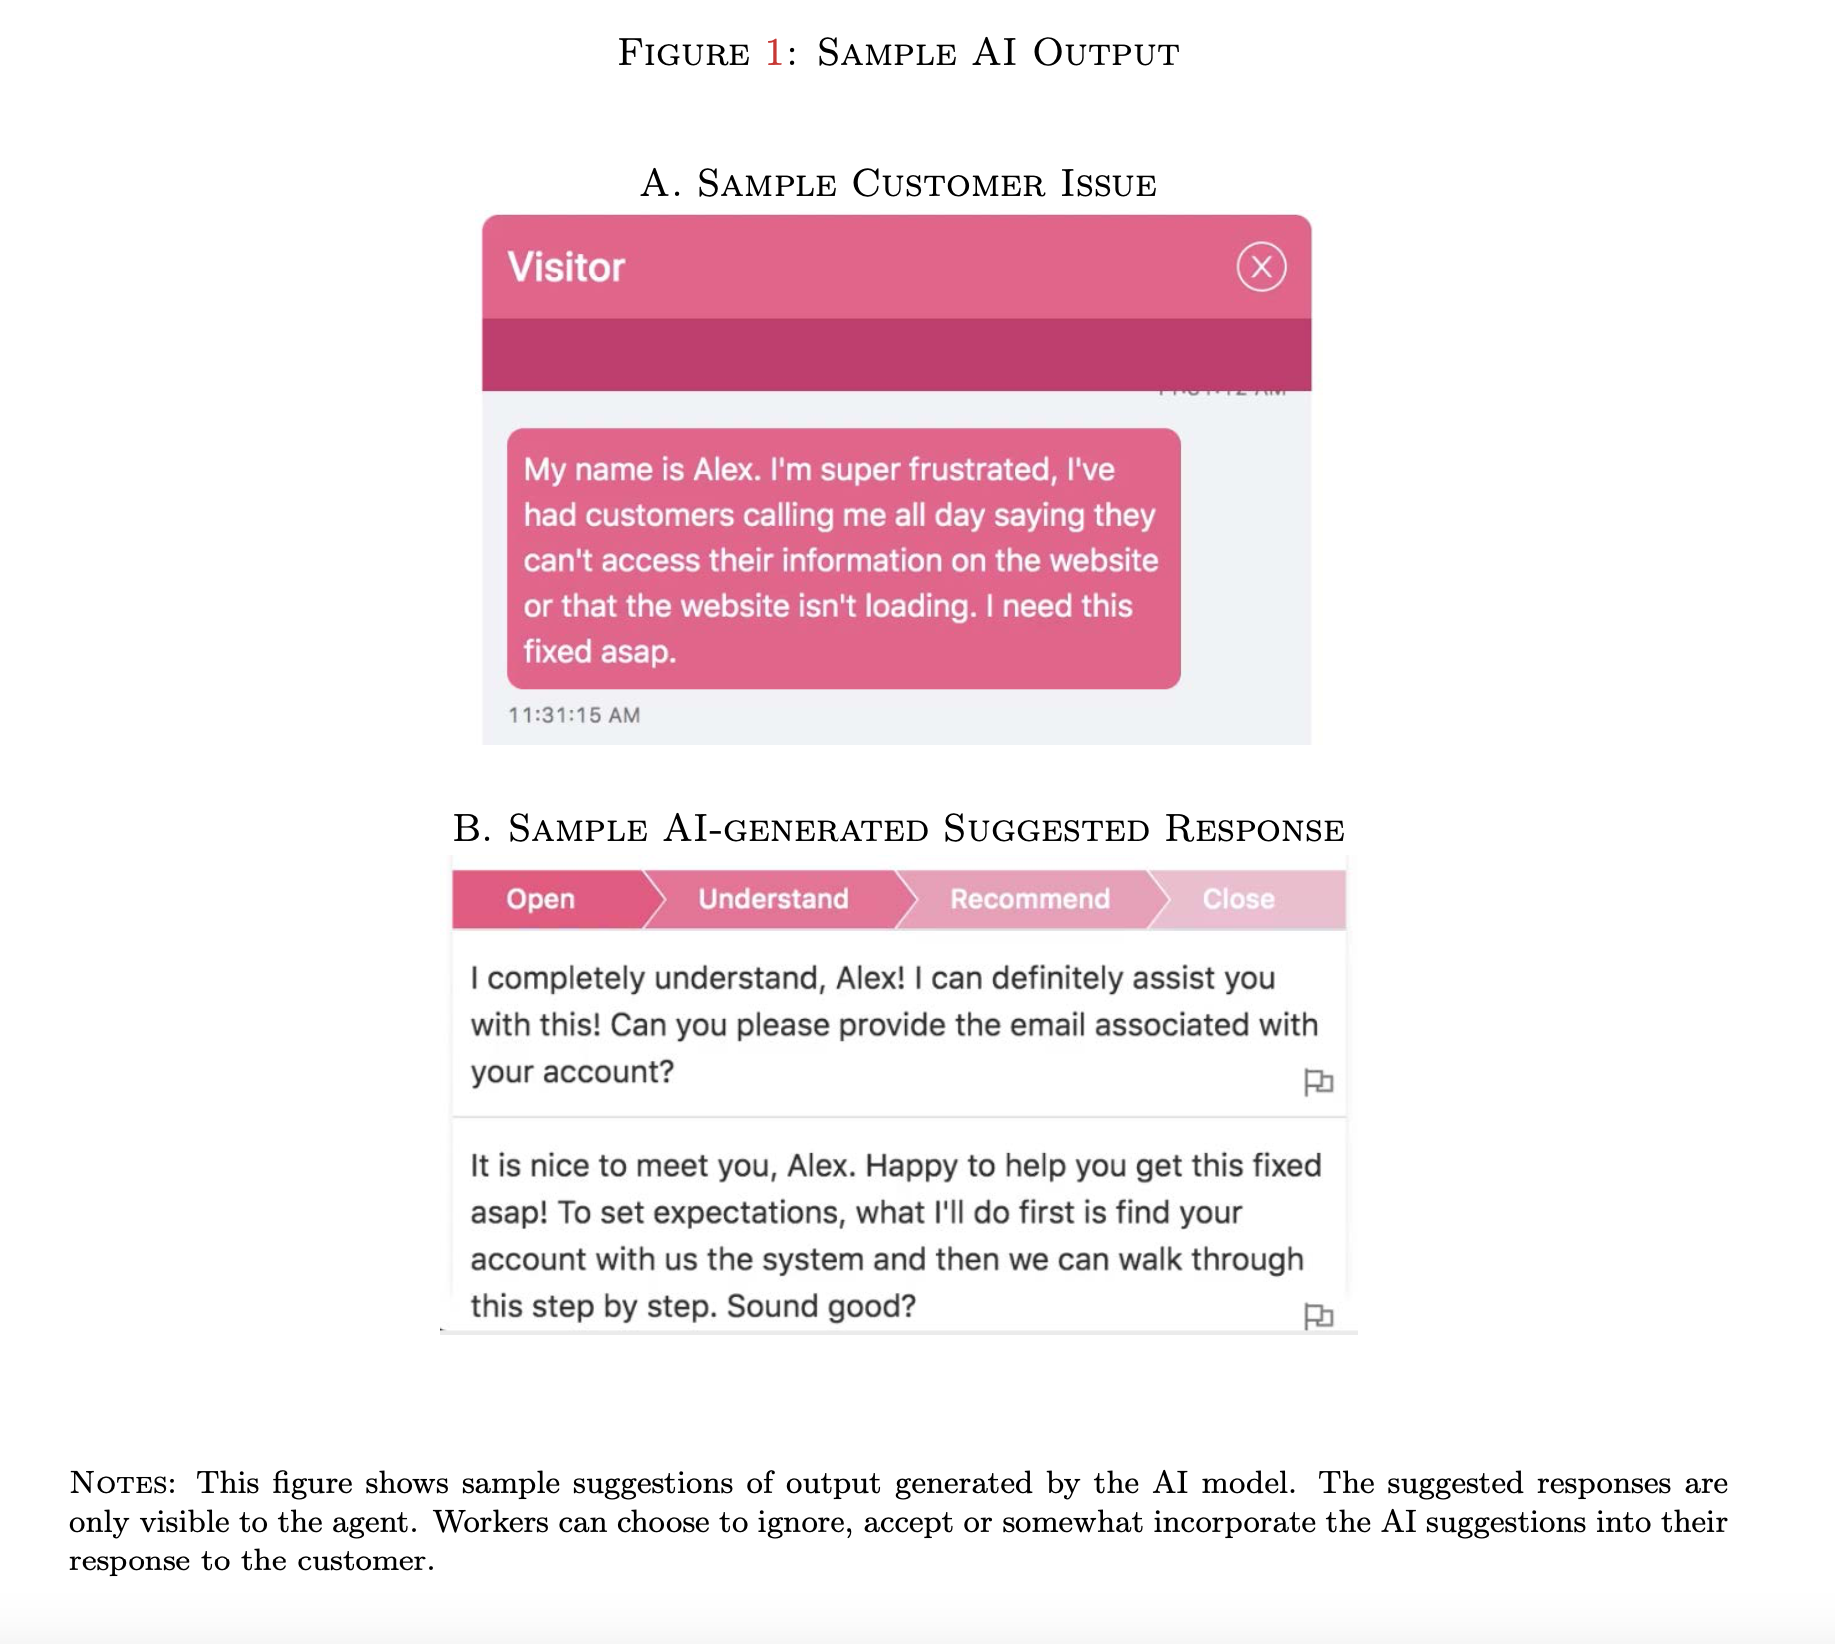
\includegraphics[scale=0.35]{./lecture_includes/brynn1}
\end{center}
\end{frame}


\begin{frame}{Rollout}
\begin{center}
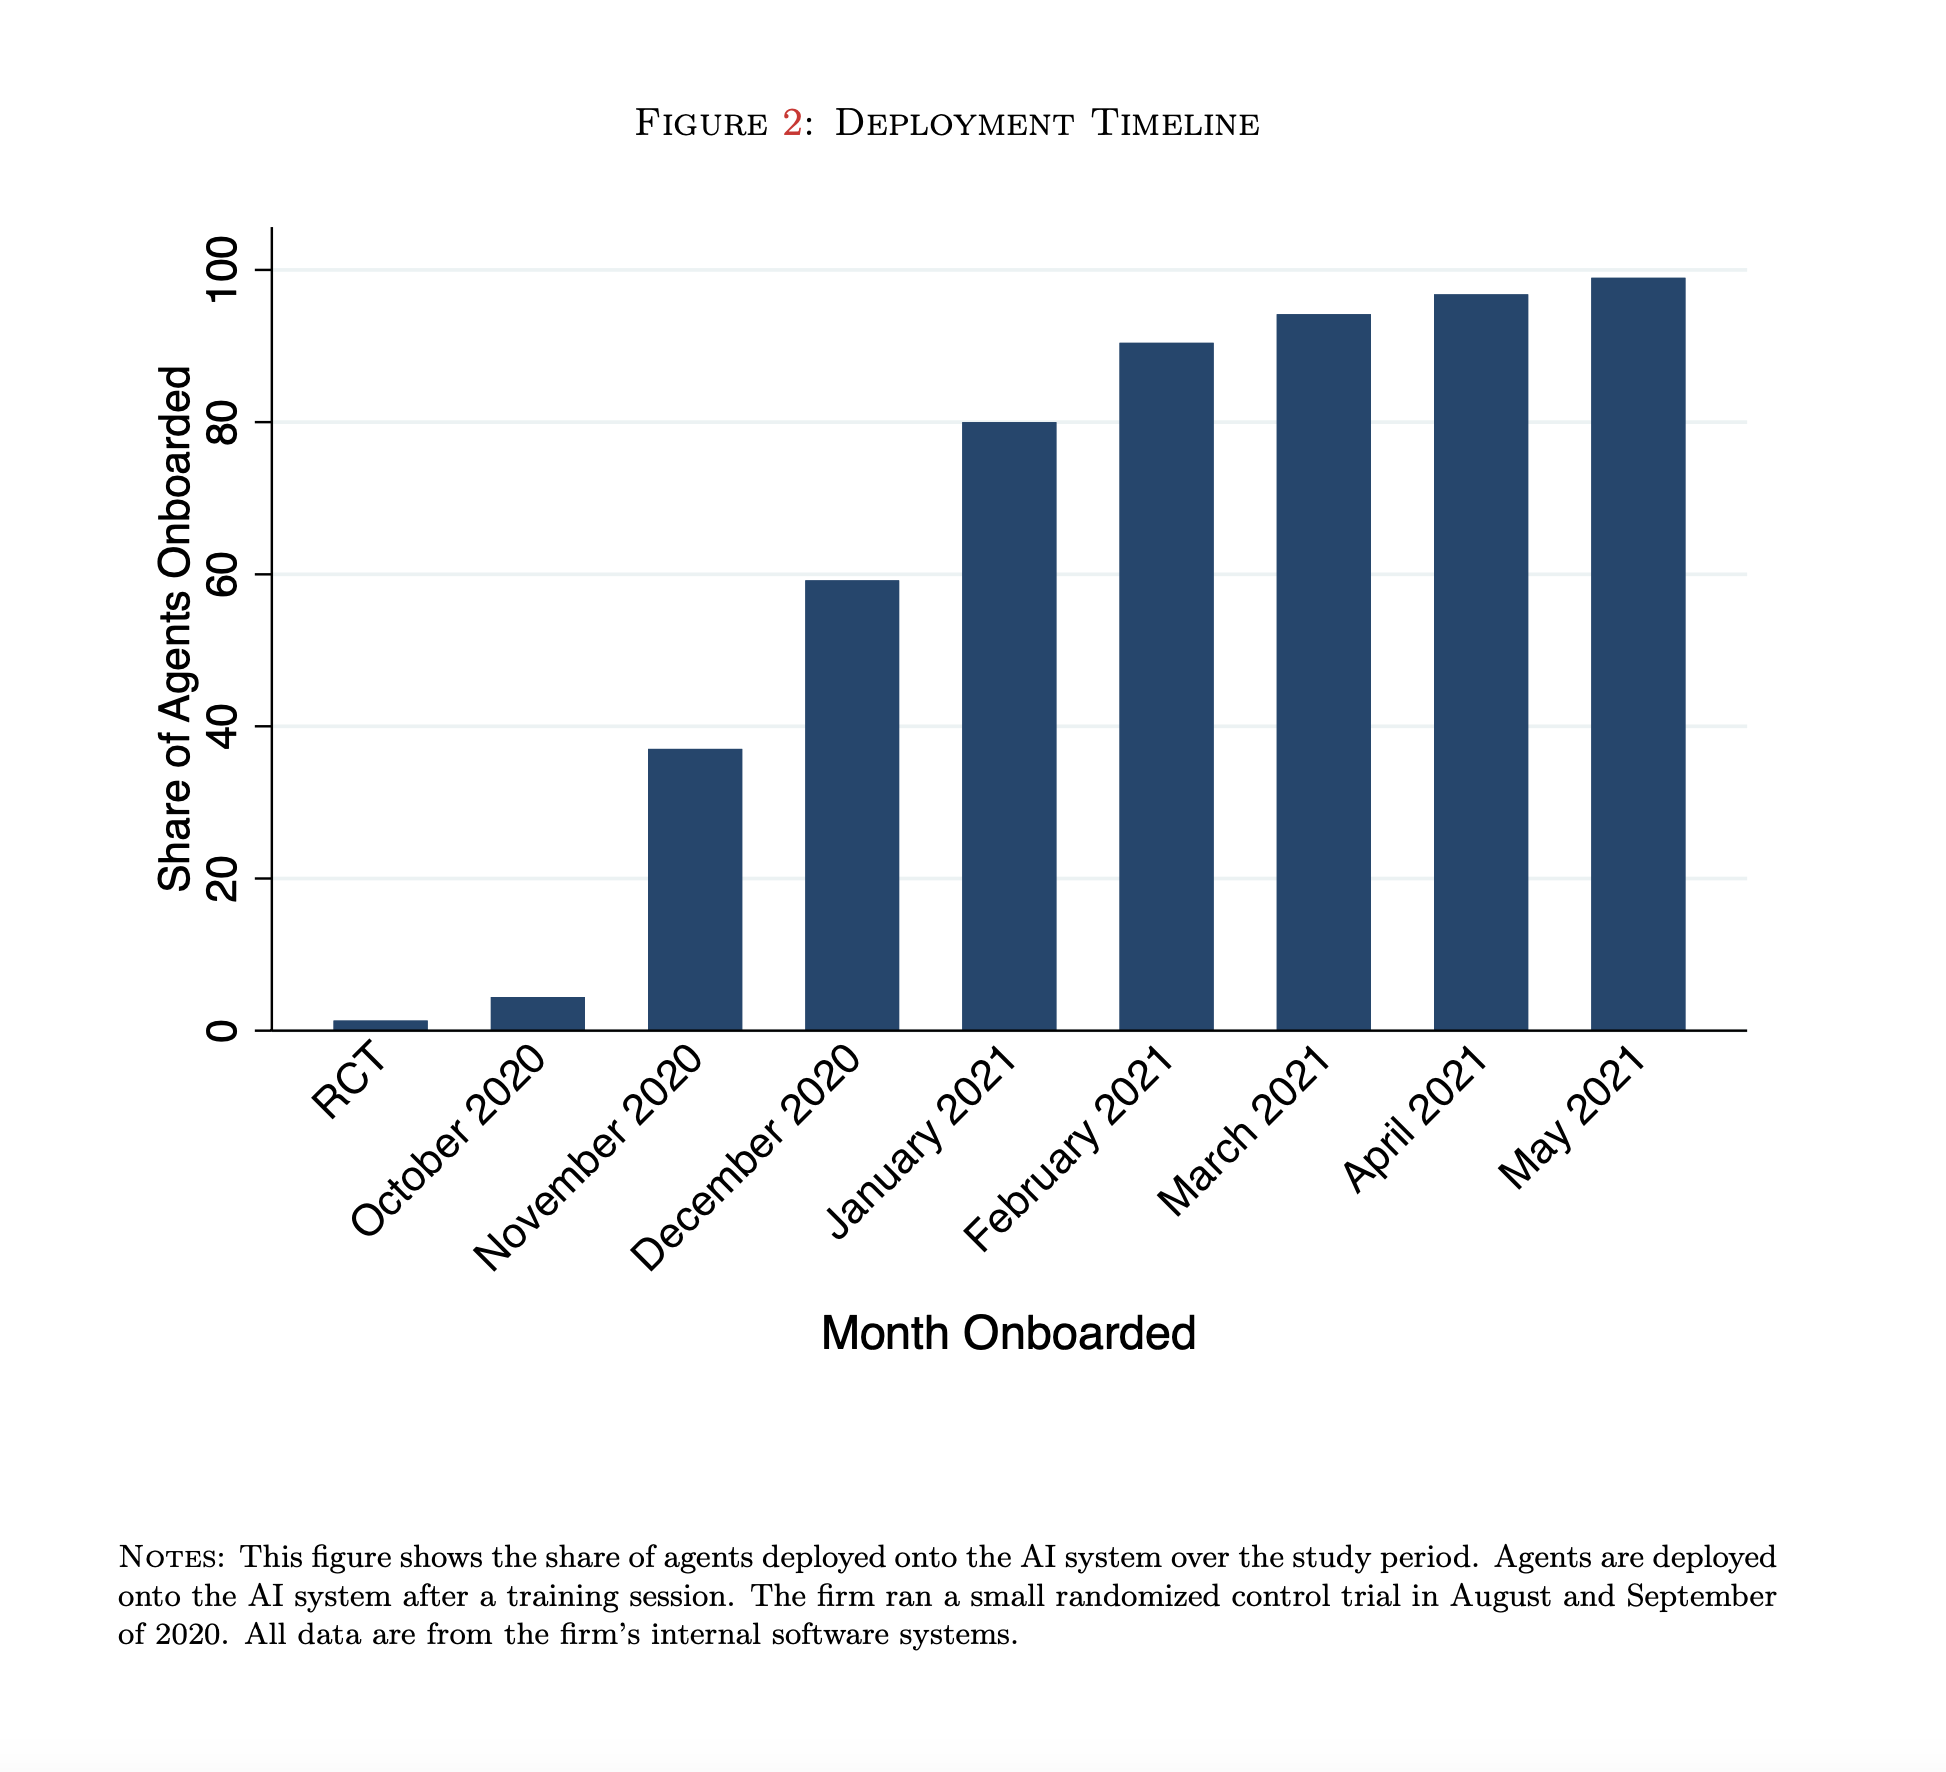
\includegraphics[scale=0.35]{./lecture_includes/brynn2}
\end{center}
\end{frame}


\begin{frame}{Resolutions of Customer Problems}
\begin{center}
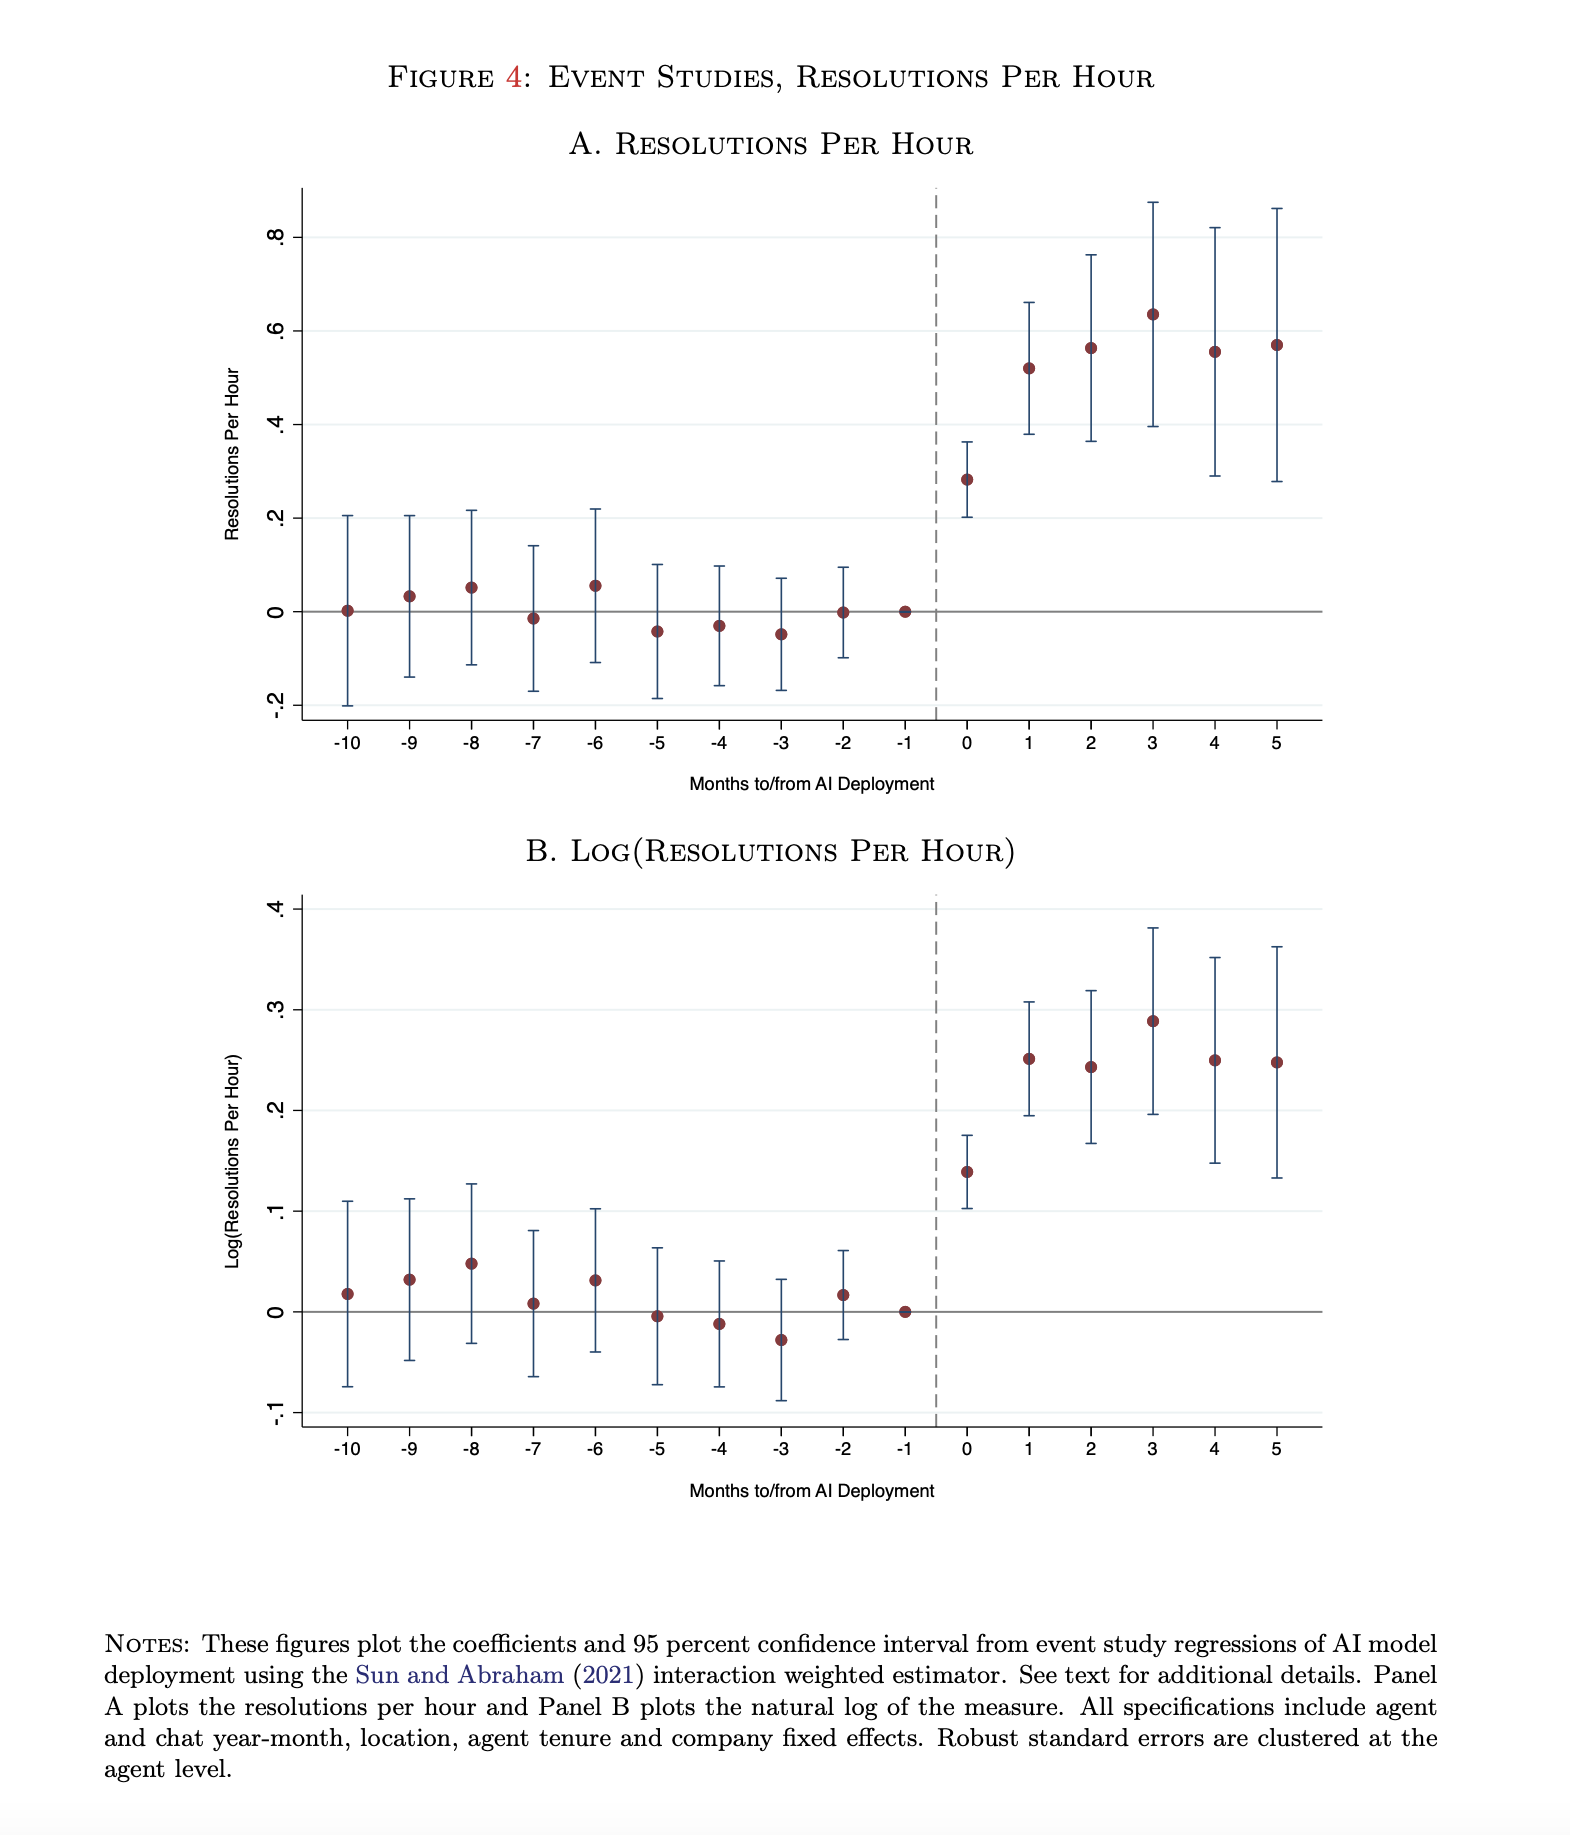
\includegraphics[scale=0.25]{./lecture_includes/brynn3}
\end{center}
\end{frame}


\begin{frame}{Additional Outcomes}
\begin{center}
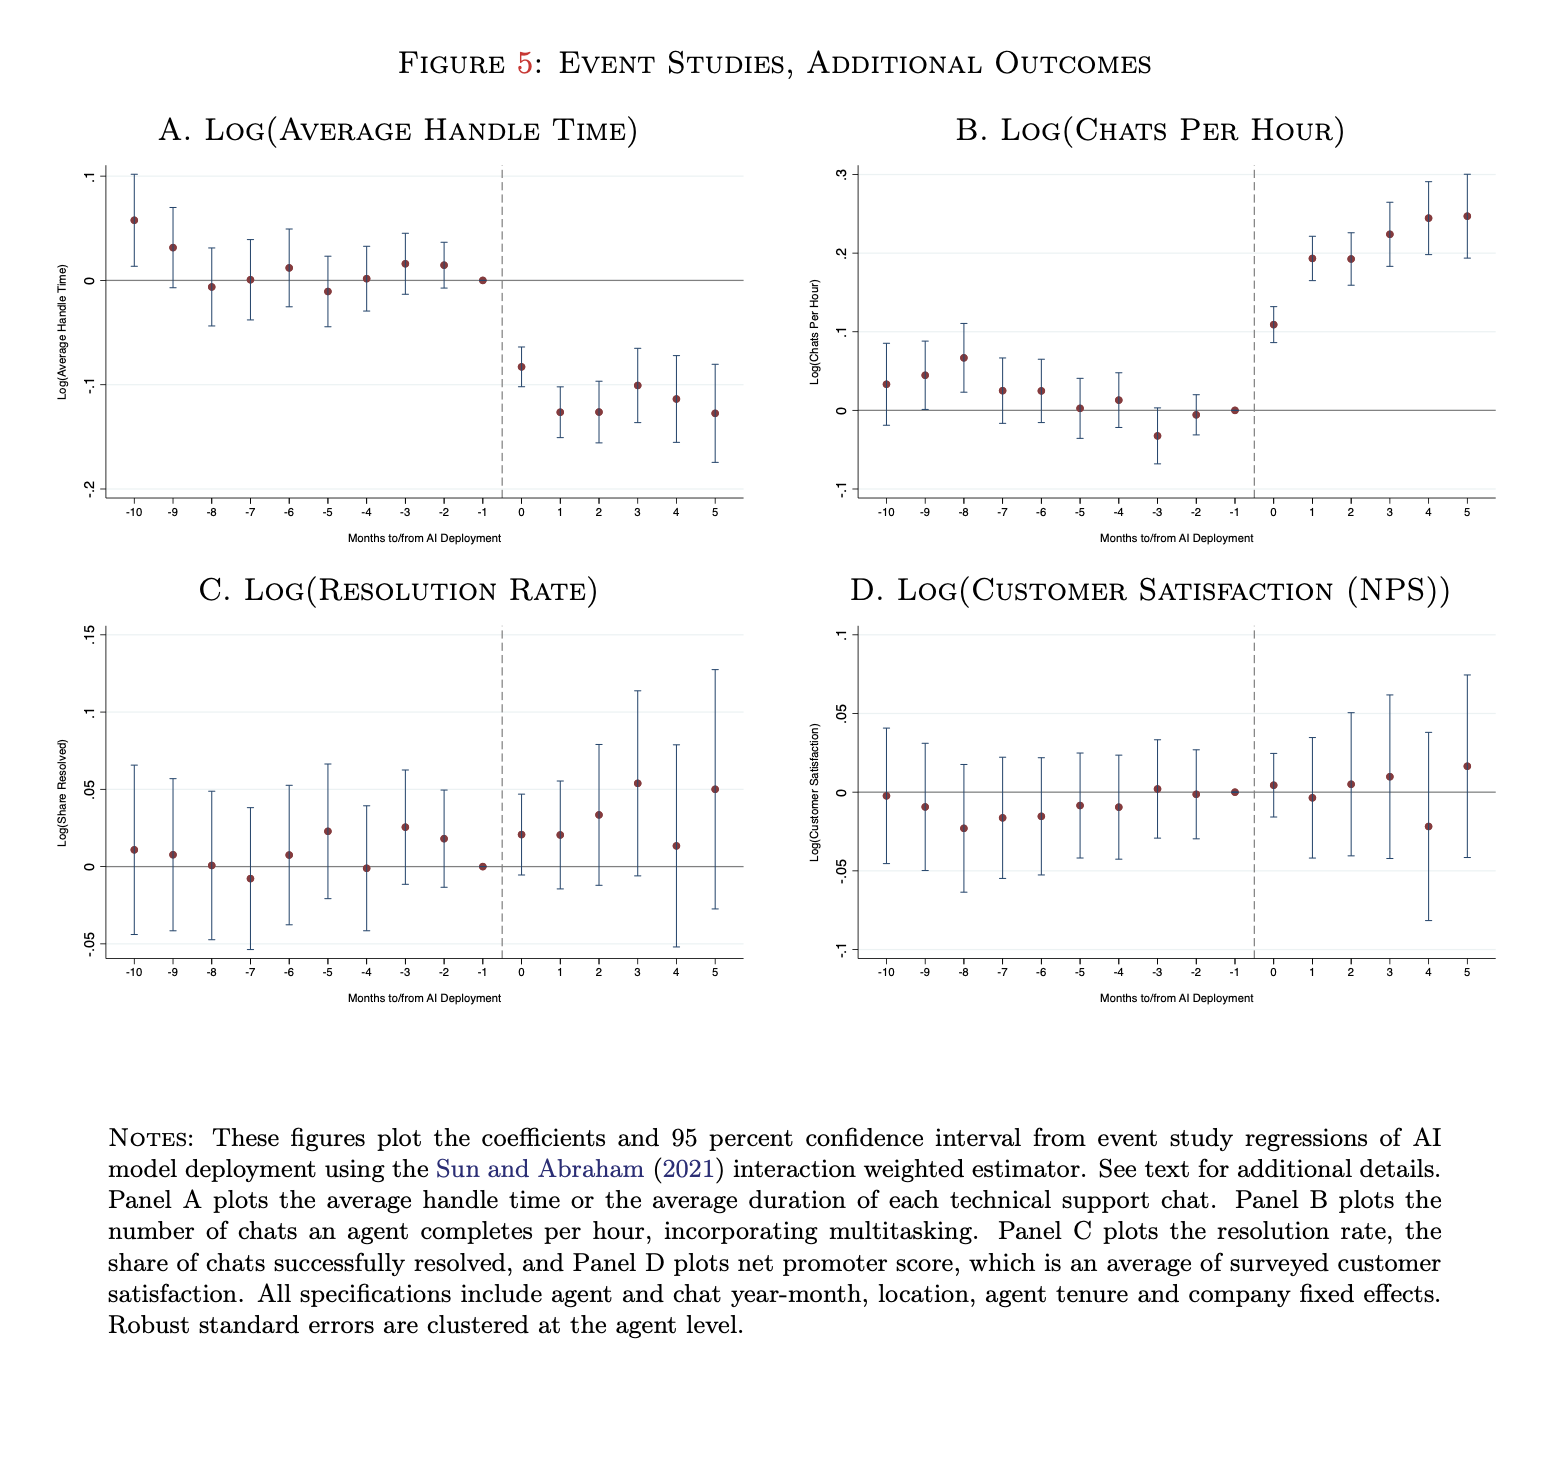
\includegraphics[scale=0.35]{./lecture_includes/brynn4}
\end{center}
\end{frame}

\begin{frame}{Heterogeneity by Skill}
\begin{center}
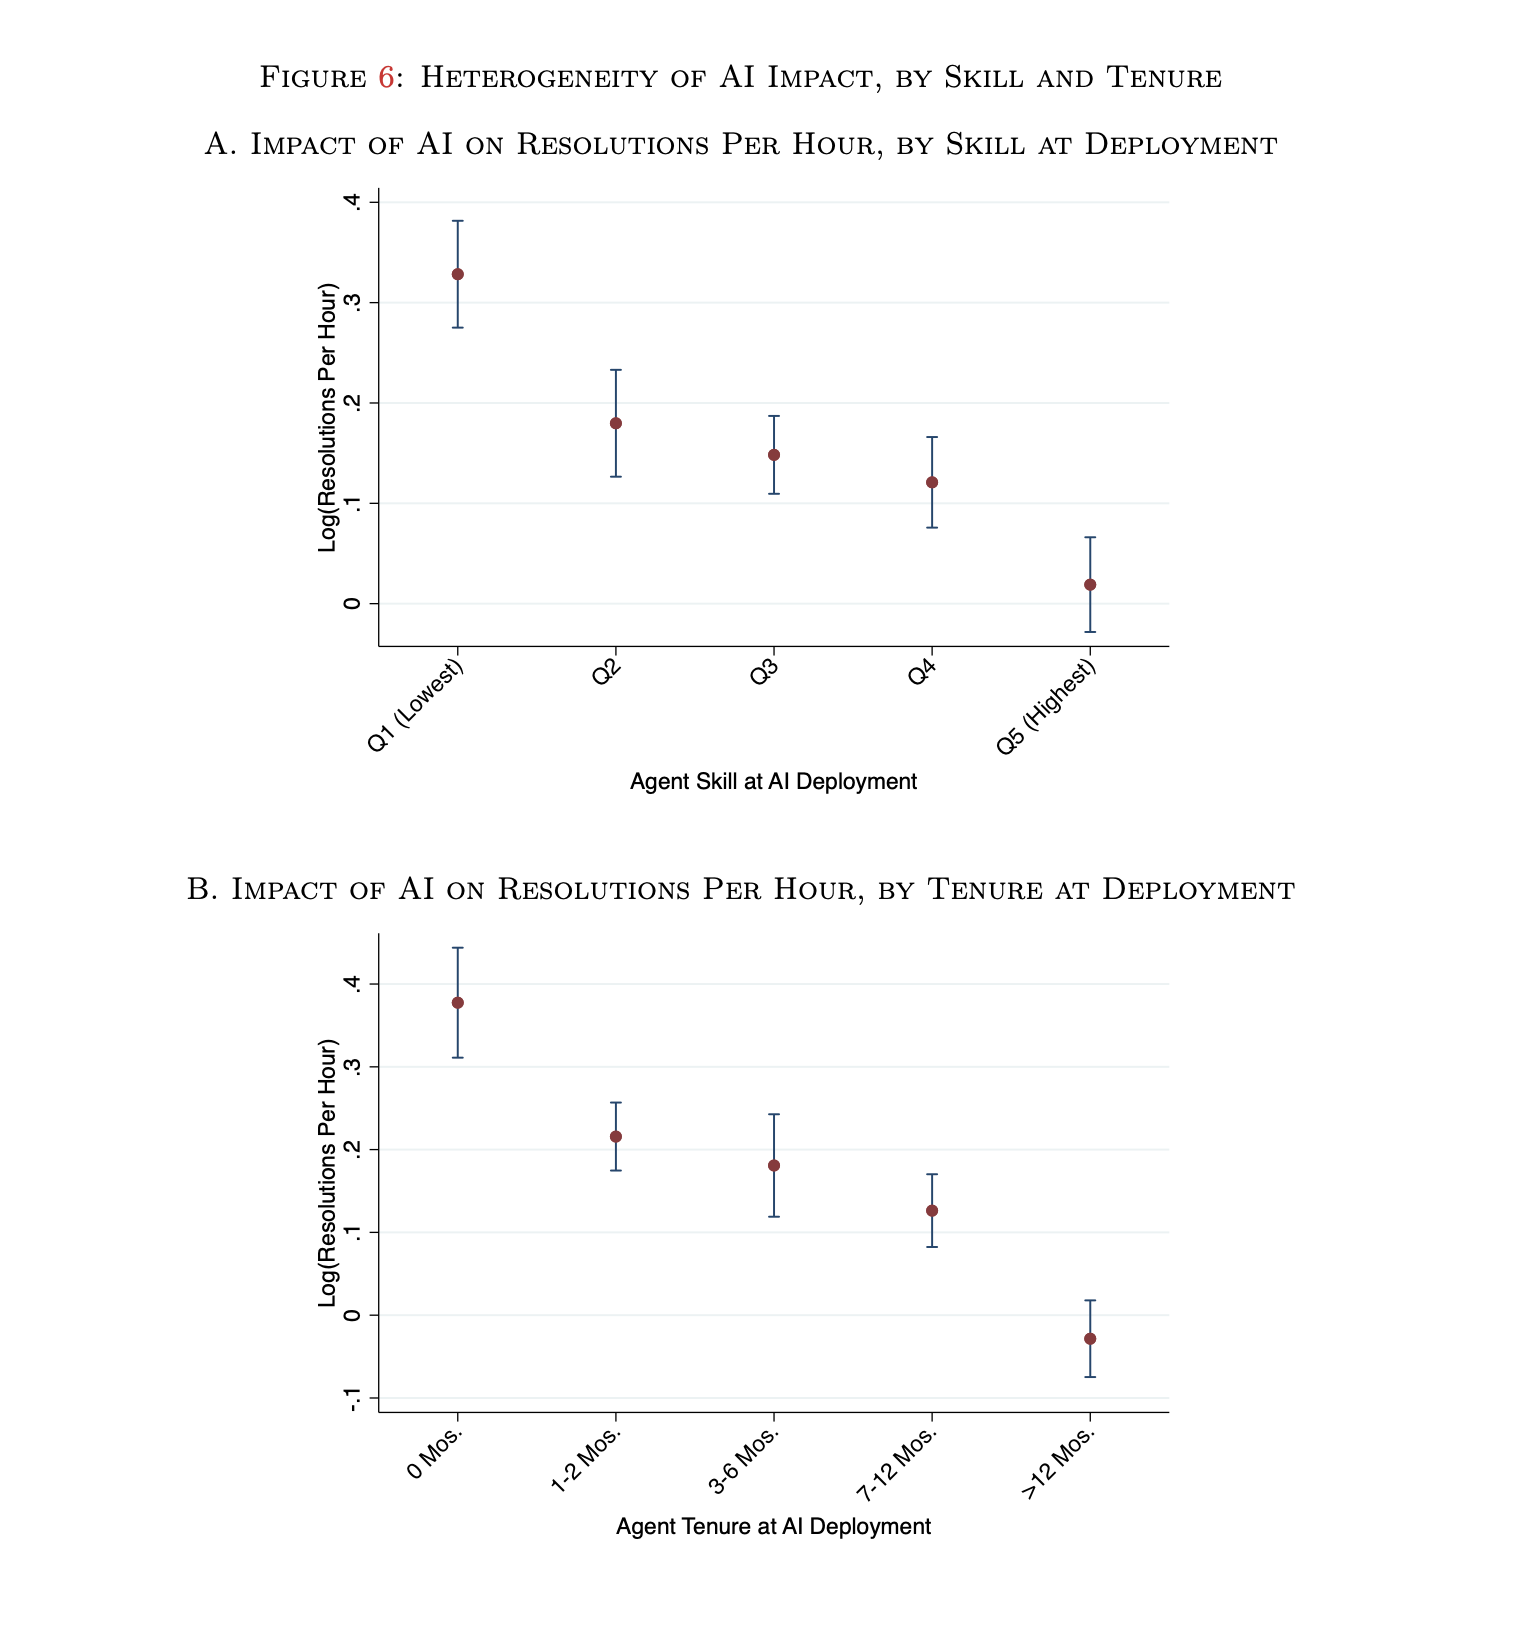
\includegraphics[scale=0.25]{./lecture_includes/brynn5}
\end{center}
\end{frame}


\begin{frame}{Heterogeneity by Skill}
\begin{center}
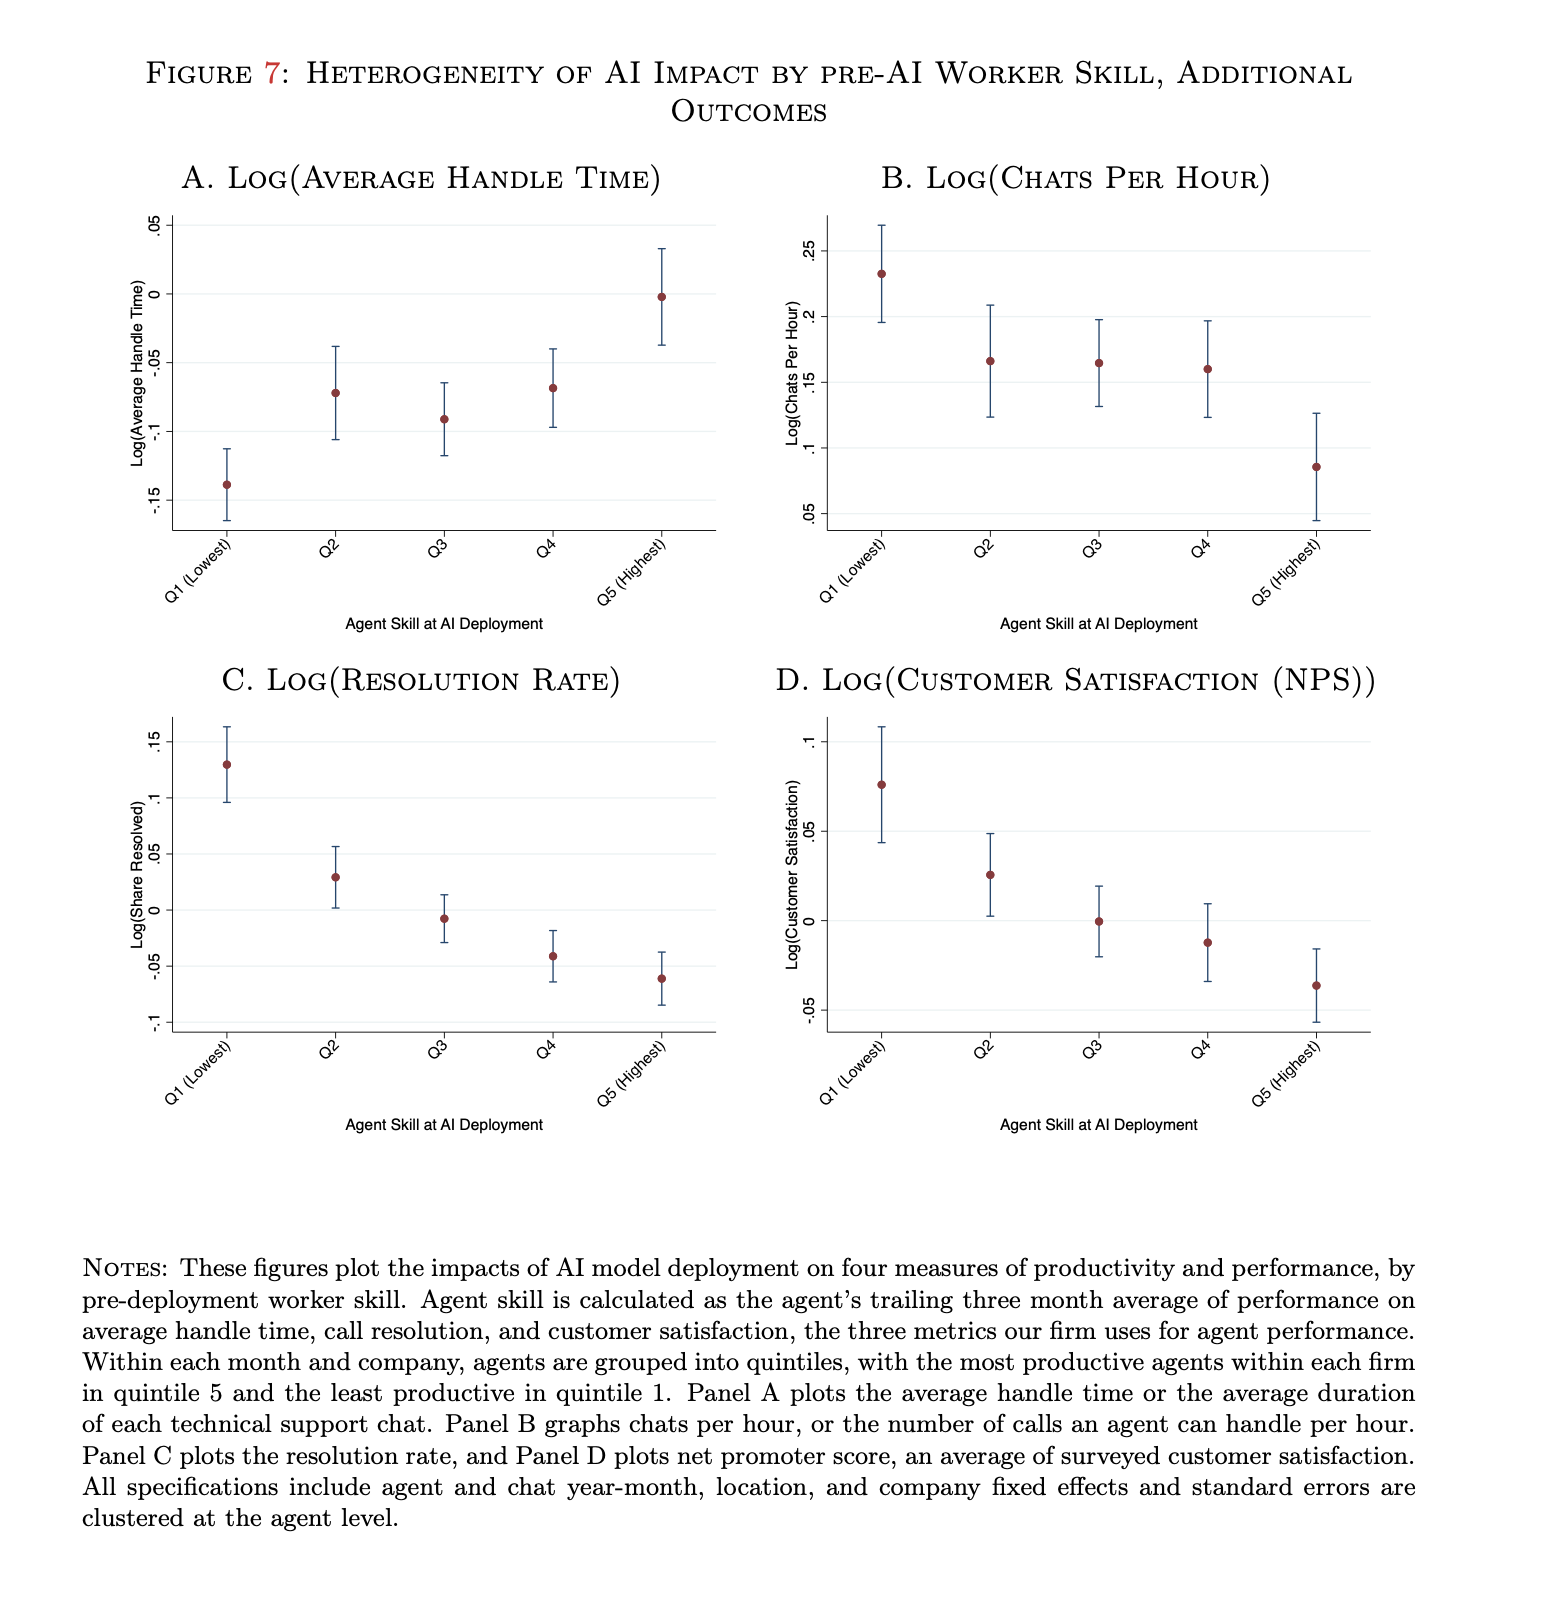
\includegraphics[scale=0.25]{./lecture_includes/brynn6}
\end{center}
\end{frame}

\begin{frame}{Heterogeneity by Worker Tenure}
\begin{center}
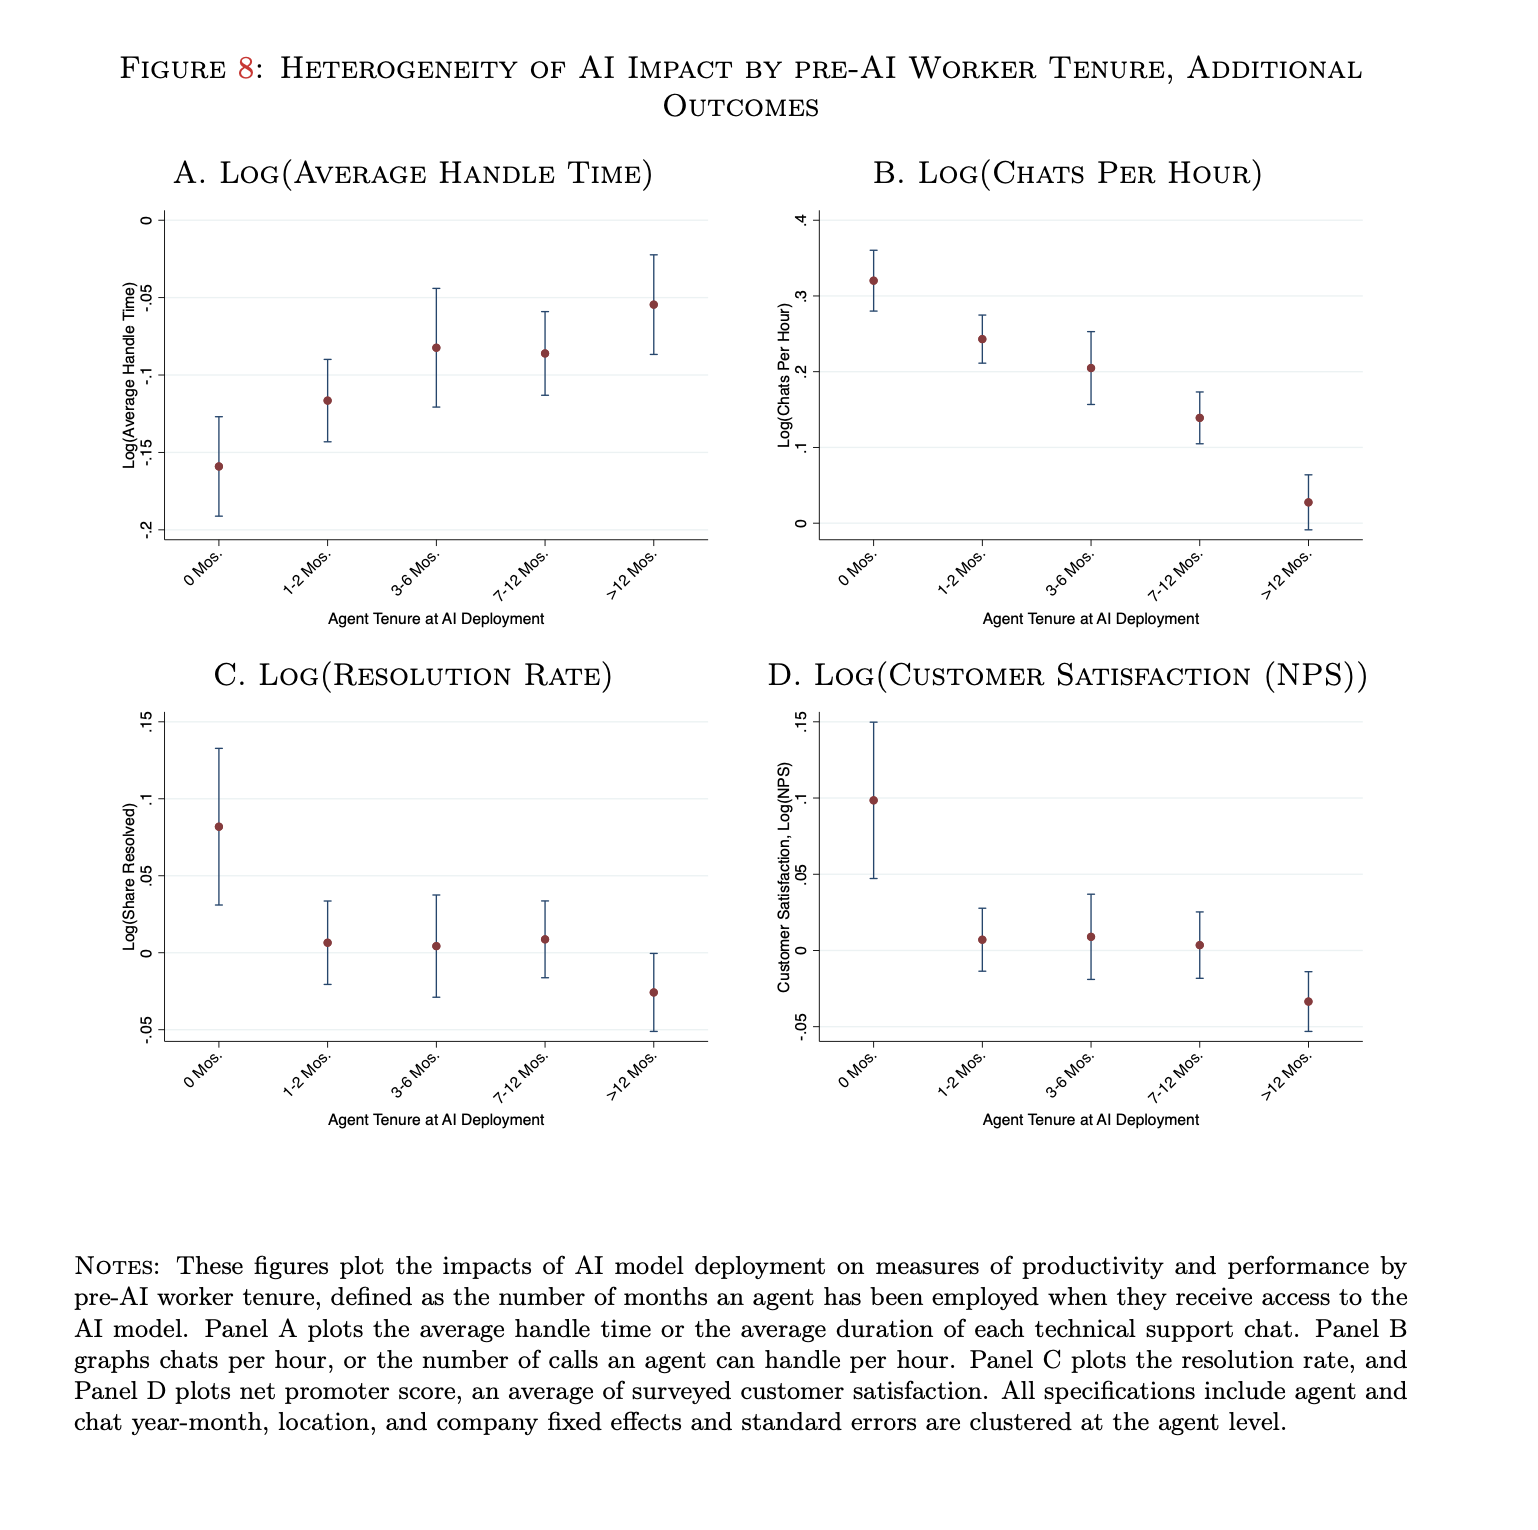
\includegraphics[scale=0.35]{./lecture_includes/brynn7}
\end{center}
\end{frame}



\begin{frame}{Sentiment}
\begin{center}
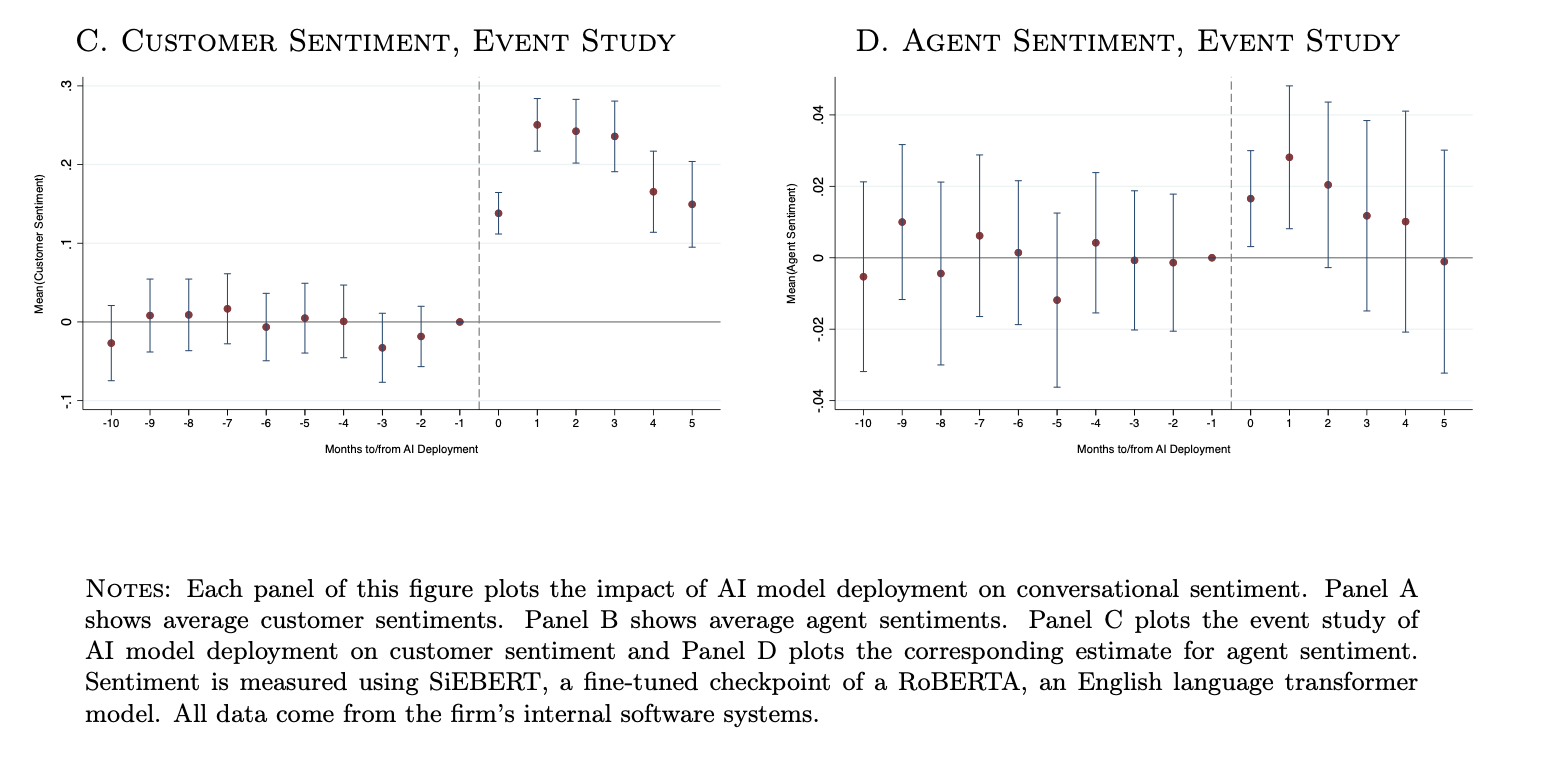
\includegraphics[scale=0.35]{./lecture_includes/brynn8}
\end{center}
\end{frame}


\begin{frame}{Sentiment}
\begin{center}
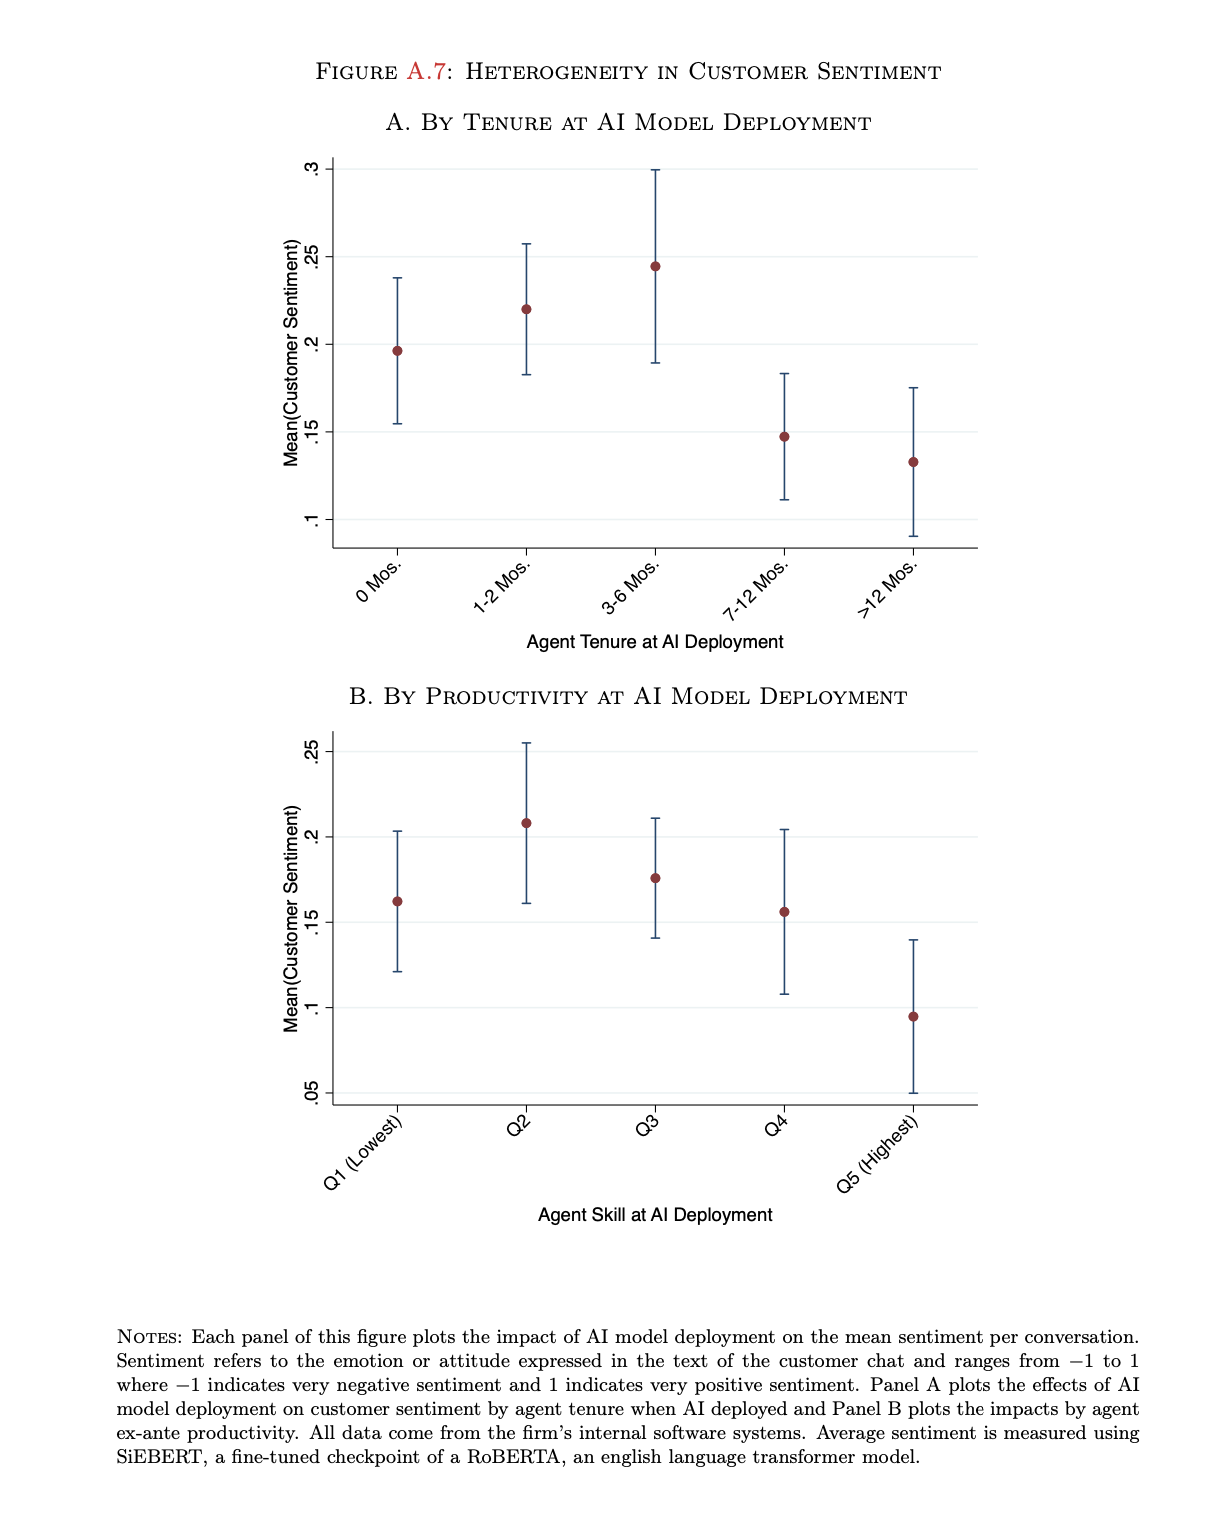
\includegraphics[scale=0.3]{./lecture_includes/brynn11}
\end{center}
\end{frame}


\begin{frame}{Manager Assistance}
\begin{center}
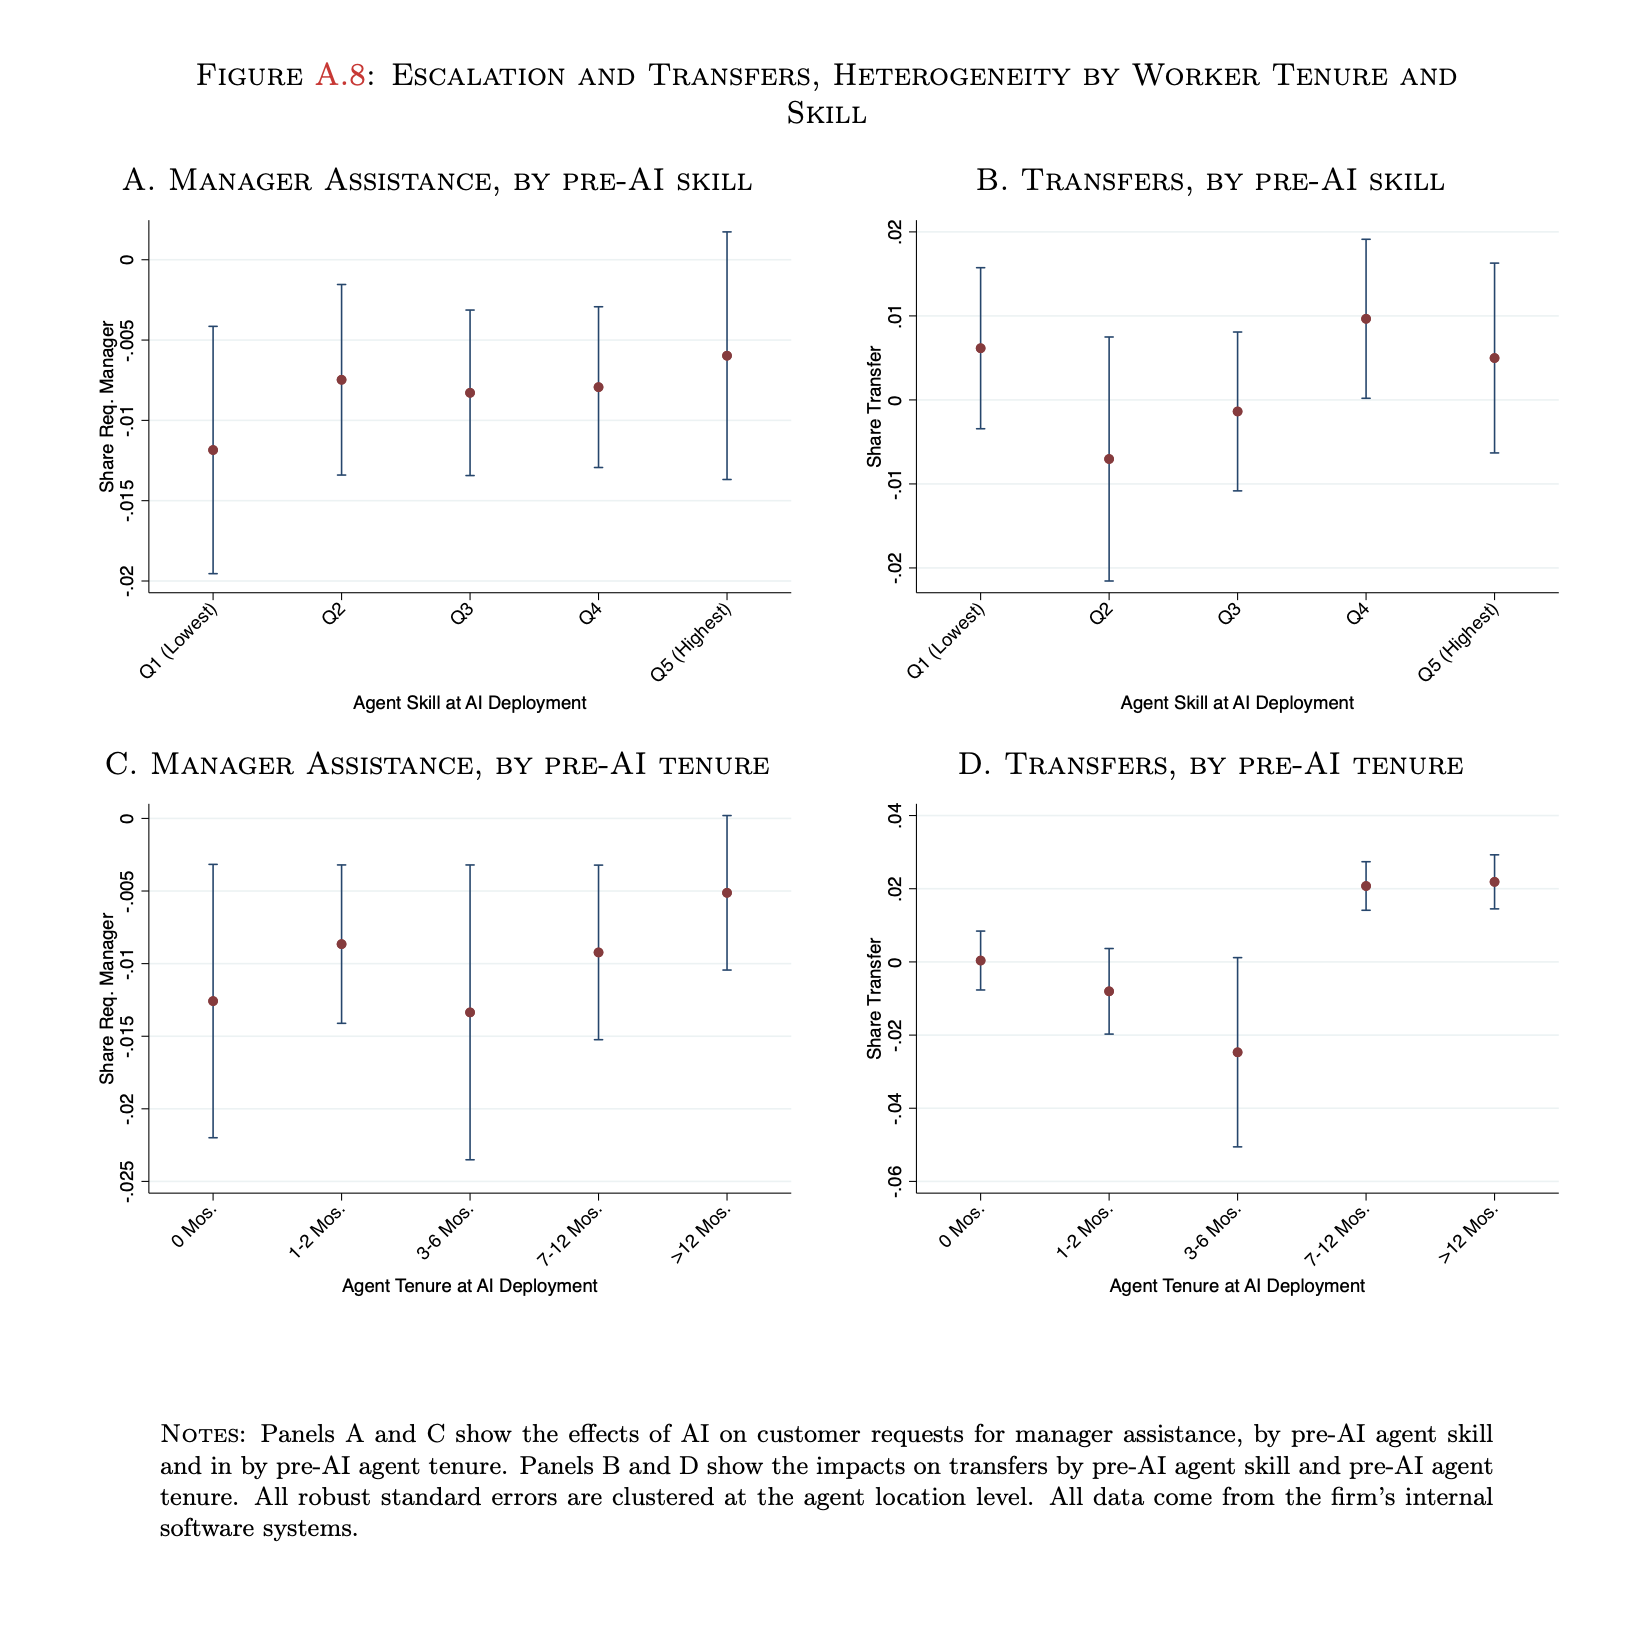
\includegraphics[scale=0.25]{./lecture_includes/brynn9}
\end{center}
\end{frame}


\begin{frame}{Outcomes}

\begin{itemize}

\item Across many dimensions, worker productivity rose
\item And the productivity increases were higher for the least skilled workers -- just like we had seen in the experiment
\item They suggest that generative AI ``reallocated experience'' to the least experienced workers making them essentially appear as though they had been their awhile
\item Findings suggest that it improves customer sentiment, reduces requests for managerial intervention, and improves employee retention
\item Still unclear how generalizeable this is, and what impact we should see on overall aggregate employment as this was AI assisted, not AI alone

\end{itemize}

\end{frame}


\section{Concluding remarks}



\begin{frame}{DiD vs ATT}

\begin{itemize}

\item We learned that difference-in-differences was just four averages and three subtractions
\item But it was also a specific regression specification
\item We saw that difference-in-differences could be used to estimate average treatment effects 
\item But the DiD equation is distinct from the ATT parameter we care about

\end{itemize}

\end{frame}


\begin{frame}{Parallel Trends}

\begin{itemize}

\item DiD only was equal to the ATT if the parallel trends assumption was true
\item But it's not verifiable so it's a difficult assumption
\item Parallel trends is not something a statistical model fixes -- it's something a control group fixes
\item Some comparison groups will satisfy parallel trends, but some won't

\end{itemize}

\end{frame}

\begin{frame}{Evidence for parallel trends}

\begin{enumerate}

\item Event study graphics -- plot coefficients and confidence intervals to check if pre-trends are zero so that post-treatment coefficients are compelling evidence for causal effects
\item Falsifications -- if possible, rule out competing hypotheses using falsifications (e.g., 65+ year olds can't be on Medicaid as they're already on Medicare)

\end{enumerate}

\end{frame}

\begin{frame}{Roadmap}

\begin{enumerate}
\item Show bite -- first order effects
\item Main results -- What's your study about?
\item Event study graphs -- This will be your main results and your evidence of parallel trends keeping in mind pre-trends and parallel trends are technically distinct
\item Falsifications -- If you can find falsifications, use them
\item Mechanisms -- can you find any explanation?
\end{enumerate}

\end{frame}

\begin{frame}{Synthetic control}

\begin{itemize}

\item But what if parallel trends really isn't realistic -- what then?
\item Then you may need to create your own control group that follows the same approximately trajectory as your treatment group pre-treatment
\item A method by Abadie and Gardazebal (2003) and follow up papers worked out a method for this called synthetic control
\item We will review that next
\end{itemize}

\end{frame}













\end{document}
